%% bare_jrnl_compsoc.tex
%% V1.3
%% 2007/01/11
%% by Michael Shell
%% See:
%% http://www.michaelshell.org/
%% for current contact information.
%%
%% This is a skeleton file demonstrating the use of IEEEtran.cls
%% (requires IEEEtran.cls version 1.7 or later) with an IEEE Computer
%% Society journal paper.
%%
%% Support sites:
%% http://www.michaelshell.org/tex/ieeetran/
%% http://www.ctan.org/tex-archive/macros/latex/contrib/IEEEtran/
%% and
%% http://www.ieee.org/

%%*************************************************************************
%% Legal Notice:
%% This code is offered as-is without any warranty either expressed or
%% implied; without even the implied warranty of MERCHANTABILITY or
%% FITNESS FOR A PARTICULAR PURPOSE! 
%% User assumes all risk.
%% In no event shall IEEE or any contributor to this code be liable for
%% any damages or losses, including, but not limited to, incidental,
%% consequential, or any other damages, resulting from the use or misuse
%% of any information contained here.
%%
%% All comments are the opinions of their respective authors and are not
%% necessarily endorsed by the IEEE.
%%
%% This work is distributed under the LaTeX Project Public License (LPPL)
%% ( http://www.latex-project.org/ ) version 1.3, and may be freely used,
%% distributed and modified. A copy of the LPPL, version 1.3, is included
%% in the base LaTeX documentation of all distributions of LaTeX released
%% 2003/12/01 or later.
%% Retain all contribution notices and credits.
%% ** Modified files should be clearly indicated as such, including  **
%% ** renaming them and changing author support contact information. **
%%
%% File list of work: IEEEtran.cls, IEEEtran_HOWTO.pdf, bare_adv.tex,
%%                    bare_conf.tex, bare_jrnl.tex, bare_jrnl_compsoc.tex
%%*************************************************************************

% *** Authors should verify (and, if needed, correct) their LaTeX system  ***
% *** with the testflow diagnostic prior to trusting their LaTeX platform ***
% *** with production work. IEEE's font choices can trigger bugs that do  ***
% *** not appear when using other class files.                            ***
% The testflow support page is at:
% http://www.michaelshell.org/tex/testflow/




% Note that the a4paper option is mainly intended so that authors in
% countries using A4 can easily print to A4 and see how their papers will
% look in print - the typesetting of the document will not typically be
% affected with changes in paper size (but the bottom and side margins will).
% Use the testflow package mentioned above to verify correct handling of
% both paper sizes by the user's LaTeX system.
%
% Also note that the "draftcls" or "draftclsnofoot", not "draft", option
% should be used if it is desired that the figures are to be displayed in
% draft mode.
%
% The Computer Society usually requires 10pt for submissions.
%
\documentclass[10pt,journal,letterpaper,compsoc]{IEEEtran}
%
% If IEEEtran.cls has not been installed into the LaTeX system files,
% manually specify the path to it like:
% \documentclass[12pt,journal,compsoc]{../sty/IEEEtran}


% Be sure to include your packages in preamble.tex
% Some very useful LaTeX packages include:
% (uncomment the ones you want to load)

\usepackage{verbatim}
\usepackage{float}
\usepackage{tabularx}
\usepackage{multirow}
\usepackage{calc}
% \usepackage{subfig}

% *** MISC UTILITY PACKAGES ***
%
%\usepackage{ifpdf}
% Heiko Oberdiek's ifpdf.sty is very useful if you need conditional
% compilation based on whether the output is pdf or dvi.
% usage:
% \ifpdf
%   % pdf code
% \else
%   % dvi code
% \fi
% The latest version of ifpdf.sty can be obtained from:
% http://www.ctan.org/tex-archive/macros/latex/contrib/oberdiek/
% Also, note that IEEEtran.cls V1.7 and later provides a builtin
% \ifCLASSINFOpdf conditional that works the same way.
% When switching from latex to pdflatex and vice-versa, the compiler may
% have to be run twice to clear warning/error messages.






% *** CITATION PACKAGES ***
%
\ifCLASSOPTIONcompsoc
  % IEEE Computer Society needs nocompress option
  % requires cite.sty v4.0 or later (November 2003)
  \usepackage[nocompress]{cite}
\else
  % normal IEEE
  % \usepackage{cite}
\fi
% cite.sty was written by Donald Arseneau
% V1.6 and later of IEEEtran pre-defines the format of the cite.sty package
% \cite{} output to follow that of IEEE. Loading the cite package will
% result in citation numbers being automatically sorted and properly
% "compressed/ranged". e.g., [1], [9], [2], [7], [5], [6] without using
% cite.sty will become [1], [2], [5]--[7], [9] using cite.sty. cite.sty's
% \cite will automatically add leading space, if needed. Use cite.sty's
% noadjust option (cite.sty V3.8 and later) if you want to turn this off.
% cite.sty is already installed on most LaTeX systems. Be sure and use
% version 4.0 (2003-05-27) and later if using hyperref.sty. cite.sty does
% not currently provide for hyperlinked citations.
% The latest version can be obtained at:
% http://www.ctan.org/tex-archive/macros/latex/contrib/cite/
% The documentation is contained in the cite.sty file itself.
%
% Note that some packages require special options to format as the Computer
% Society requires. In particular, Computer Society  papers do not use
% compressed citation ranges as is done in typical IEEE papers
% (e.g., [1]-[4]). Instead, they list every citation separately in order
% (e.g., [1], [2], [3], [4]). To get the latter we need to load the cite
% package with the nocompress option which is supported by cite.sty v4.0
% and later. Note also the use of a CLASSOPTION conditional provided by
% IEEEtran.cls V1.7 and later.





% *** GRAPHICS RELATED PACKAGES ***
%
\ifCLASSINFOpdf
  \usepackage[pdftex]{graphicx}
  % declare the path(s) where your graphic files are
  \graphicspath{{./figures/}}
  % and their extensions so you won't have to specify these with
  % every instance of \includegraphics
  \DeclareGraphicsExtensions{.pdf,.jpeg,.png}
\else
  % or other class option (dvipsone, dvipdf, if not using dvips). graphicx
  % will default to the driver specified in the system graphics.cfg if no
  % driver is specified.
  % \usepackage[dvips]{graphicx}
  % declare the path(s) where your graphic files are
  % \graphicspath{{../eps/}}
  % and their extensions so you won't have to specify these with
  % every instance of \includegraphics
  % \DeclareGraphicsExtensions{.eps}
\fi
% graphicx was written by David Carlisle and Sebastian Rahtz. It is
% required if you want graphics, photos, etc. graphicx.sty is already
% installed on most LaTeX systems. The latest version and documentation can
% be obtained at: 
% http://www.ctan.org/tex-archive/macros/latex/required/graphics/
% Another good source of documentation is "Using Imported Graphics in
% LaTeX2e" by Keith Reckdahl which can be found as epslatex.ps or
% epslatex.pdf at: http://www.ctan.org/tex-archive/info/
%
% latex, and pdflatex in dvi mode, support graphics in encapsulated
% postscript (.eps) format. pdflatex in pdf mode supports graphics
% in .pdf, .jpeg, .png and .mps (metapost) formats. Users should ensure
% that all non-photo figures use a vector format (.eps, .pdf, .mps) and
% not a bitmapped formats (.jpeg, .png). IEEE frowns on bitmapped formats
% which can result in "jaggedy"/blurry rendering of lines and letters as
% well as large increases in file sizes.
%
% You can find documentation about the pdfTeX application at:
% http://www.tug.org/applications/pdftex





% *** MATH PACKAGES ***
%
\usepackage[cmex10]{amsmath}
% A popular package from the American Mathematical Society that provides
% many useful and powerful commands for dealing with mathematics. If using
% it, be sure to load this package with the cmex10 option to ensure that
% only type 1 fonts will utilized at all point sizes. Without this option,
% it is possible that some math symbols, particularly those within
% footnotes, will be rendered in bitmap form which will result in a
% document that can not be IEEE Xplore compliant!
%
% Also, note that the amsmath package sets \interdisplaylinepenalty to 10000
% thus preventing page breaks from occurring within multiline equations. Use:
%\interdisplaylinepenalty=2500
% after loading amsmath to restore such page breaks as IEEEtran.cls normally
% does. amsmath.sty is already installed on most LaTeX systems. The latest
% version and documentation can be obtained at:
% http://www.ctan.org/tex-archive/macros/latex/required/amslatex/math/





% *** SPECIALIZED LIST PACKAGES ***
%
%\usepackage{algorithmic}
% algorithmic.sty was written by Peter Williams and Rogerio Brito.
% This package provides an algorithmic environment fo describing algorithms.
% You can use the algorithmic environment in-text or within a figure
% environment to provide for a floating algorithm. Do NOT use the algorithm
% floating environment provided by algorithm.sty (by the same authors) or
% algorithm2e.sty (by Christophe Fiorio) as IEEE does not use dedicated
% algorithm float types and packages that provide these will not provide
% correct IEEE style captions. The latest version and documentation of
% algorithmic.sty can be obtained at:
% http://www.ctan.org/tex-archive/macros/latex/contrib/algorithms/
% There is also a support site at:
% http://algorithms.berlios.de/index.html
% Also of interest may be the (relatively newer and more customizable)
% algorithmicx.sty package by Szasz Janos:
% http://www.ctan.org/tex-archive/macros/latex/contrib/algorithmicx/




% *** ALIGNMENT PACKAGES ***
%
%\usepackage{array}
% Frank Mittelbach's and David Carlisle's array.sty patches and improves
% the standard LaTeX2e array and tabular environments to provide better
% appearance and additional user controls. As the default LaTeX2e table
% generation code is lacking to the point of almost being broken with
% respect to the quality of the end results, all users are strongly
% advised to use an enhanced (at the very least that provided by array.sty)
% set of table tools. array.sty is already installed on most systems. The
% latest version and documentation can be obtained at:
% http://www.ctan.org/tex-archive/macros/latex/required/tools/


\usepackage{mdwmath}
\usepackage{mdwtab}
% Also highly recommended is Mark Wooding's extremely powerful MDW tools,
% especially mdwmath.sty and mdwtab.sty which are used to format equations
% and tables, respectively. The MDWtools set is already installed on most
% LaTeX systems. The lastest version and documentation is available at:
% http://www.ctan.org/tex-archive/macros/latex/contrib/mdwtools/


% IEEEtran contains the IEEEeqnarray family of commands that can be used to
% generate multiline equations as well as matrices, tables, etc., of high
% quality.


\usepackage{eqparbox}
% Also of notable interest is Scott Pakin's eqparbox package for creating
% (automatically sized) equal width boxes - aka "natural width parboxes".
% Available at:
% http://www.ctan.org/tex-archive/macros/latex/contrib/eqparbox/





% *** SUBFIGURE PACKAGES ***
\ifCLASSOPTIONcompsoc
\usepackage[tight,normalsize,sf,SF]{subfigure}
\else
\usepackage[tight,footnotesize]{subfigure}
\fi
% subfigure.sty was written by Steven Douglas Cochran. This package makes it
% easy to put subfigures in your figures. e.g., "Figure 1a and 1b". For IEEE
% work, it is a good idea to load it with the tight package option to reduce
% the amount of white space around the subfigures. Computer Society papers
% use a larger font and \sffamily font for their captions, hence the
% additional options needed under compsoc mode. subfigure.sty is already
% installed on most LaTeX systems. The latest version and documentation can
% be obtained at:
% http://www.ctan.org/tex-archive/obsolete/macros/latex/contrib/subfigure/
% subfigure.sty has been superceeded by subfig.sty.


%\ifCLASSOPTIONcompsoc
%  \usepackage[caption=false]{caption}
%  \usepackage[font=normalsize,labelfont=sf,textfont=sf]{subfig}
%\else
%  \usepackage[caption=false]{caption}
%  \usepackage[font=footnotesize]{subfig}
%\fi
% subfig.sty, also written by Steven Douglas Cochran, is the modern
% replacement for subfigure.sty. However, subfig.sty requires and
% automatically loads Axel Sommerfeldt's caption.sty which will override
% IEEEtran.cls handling of captions and this will result in nonIEEE style
% figure/table captions. To prevent this problem, be sure and preload
% caption.sty with its "caption=false" package option. This is will preserve
% IEEEtran.cls handing of captions. Version 1.3 (2005/06/28) and later 
% (recommended due to many improvements over 1.2) of subfig.sty supports
% the caption=false option directly:
%\ifCLASSOPTIONcompsoc
%  \usepackage[caption=false,font=normalsize,labelfont=sf,textfont=sf]{subfig}
%\else
%  \usepackage[caption=false,font=footnotesize]{subfig}
%\fi
%
% The latest version and documentation can be obtained at:
% http://www.ctan.org/tex-archive/macros/latex/contrib/subfig/
% The latest version and documentation of caption.sty can be obtained at:
% http://www.ctan.org/tex-archive/macros/latex/contrib/caption/




% *** FLOAT PACKAGES ***
%
%\usepackage{fixltx2e}
% fixltx2e, the successor to the earlier fix2col.sty, was written by
% Frank Mittelbach and David Carlisle. This package corrects a few problems
% in the LaTeX2e kernel, the most notable of which is that in current
% LaTeX2e releases, the ordering of single and double column floats is not
% guaranteed to be preserved. Thus, an unpatched LaTeX2e can allow a
% single column figure to be placed prior to an earlier double column
% figure. The latest version and documentation can be found at:
% http://www.ctan.org/tex-archive/macros/latex/base/



%\usepackage{stfloats}
% stfloats.sty was written by Sigitas Tolusis. This package gives LaTeX2e
% the ability to do double column floats at the bottom of the page as well
% as the top. (e.g., "\begin{figure*}[!b]" is not normally possible in
% LaTeX2e). It also provides a command:
%\fnbelowfloat
% to enable the placement of footnotes below bottom floats (the standard
% LaTeX2e kernel puts them above bottom floats). This is an invasive package
% which rewrites many portions of the LaTeX2e float routines. It may not work
% with other packages that modify the LaTeX2e float routines. The latest
% version and documentation can be obtained at:
% http://www.ctan.org/tex-archive/macros/latex/contrib/sttools/
% Documentation is contained in the stfloats.sty comments as well as in the
% presfull.pdf file. Do not use the stfloats baselinefloat ability as IEEE
% does not allow \baselineskip to stretch. Authors submitting work to the
% IEEE should note that IEEE rarely uses double column equations and
% that authors should try to avoid such use. Do not be tempted to use the
% cuted.sty or midfloat.sty packages (also by Sigitas Tolusis) as IEEE does
% not format its papers in such ways.




%\ifCLASSOPTIONcaptionsoff
%  \usepackage[nomarkers]{endfloat}
% \let\MYoriglatexcaption\caption
% \renewcommand{\caption}[2][\relax]{\MYoriglatexcaption[#2]{#2}}
%\fi
% endfloat.sty was written by James Darrell McCauley and Jeff Goldberg.
% This package may be useful when used in conjunction with IEEEtran.cls'
% captionsoff option. Some IEEE journals/societies require that submissions
% have lists of figures/tables at the end of the paper and that
% figures/tables without any captions are placed on a page by themselves at
% the end of the document. If needed, the draftcls IEEEtran class option or
% \CLASSINPUTbaselinestretch interface can be used to increase the line
% spacing as well. Be sure and use the nomarkers option of endfloat to
% prevent endfloat from "marking" where the figures would have been placed
% in the text. The two hack lines of code above are a slight modification of
% that suggested by in the endfloat docs (section 8.3.1) to ensure that
% the full captions always appear in the list of figures/tables - even if
% the user used the short optional argument of \caption[]{}.
% IEEE papers do not typically make use of \caption[]'s optional argument,
% so this should not be an issue. A similar trick can be used to disable
% captions of packages such as subfig.sty that lack options to turn off
% the subcaptions:
% For subfig.sty:
% \let\MYorigsubfloat\subfloat
% \renewcommand{\subfloat}[2][\relax]{\MYorigsubfloat[]{#2}}
% For subfigure.sty:
% \let\MYorigsubfigure\subfigure
% \renewcommand{\subfigure}[2][\relax]{\MYorigsubfigure[]{#2}}
% However, the above trick will not work if both optional arguments of
% the \subfloat/subfig command are used. Furthermore, there needs to be a
% description of each subfigure *somewhere* and endfloat does not add
% subfigure captions to its list of figures. Thus, the best approach is to
% avoid the use of subfigure captions (many IEEE journals avoid them anyway)
% and instead reference/explain all the subfigures within the main caption.
% The latest version of endfloat.sty and its documentation can obtained at:
% http://www.ctan.org/tex-archive/macros/latex/contrib/endfloat/
%
% The IEEEtran \ifCLASSOPTIONcaptionsoff conditional can also be used
% later in the document, say, to conditionally put the References on a 
% page by themselves.




% *** PDF, URL AND HYPERLINK PACKAGES ***
%
\usepackage{url}
% url.sty was written by Donald Arseneau. It provides better support for
% handling and breaking URLs. url.sty is already installed on most LaTeX
% systems. The latest version can be obtained at:
% http://www.ctan.org/tex-archive/macros/latex/contrib/misc/
% Read the url.sty source comments for usage information. Basically,
% \url{my_url_here}.





% *** Do not adjust lengths that control margins, column widths, etc. ***
% *** Do not use packages that alter fonts (such as pslatex).         ***
% There should be no need to do such things with IEEEtran.cls V1.6 and later.
% (Unless specifically asked to do so by the journal or conference you plan
% to submit to, of course. )


% correct bad hyphenation here
\hyphenation{op-tical net-works semi-conduc-tor overload socio technical inte-gra-tion}

\floatstyle{ruled}
\newfloat{placeholder}{thp}{lop}
\floatname{placeholder}{Box}


%


\begin{document}
\newcommand{\TODO}[1]{\noindent\textbf{TODO:} \emph{#1}}
\newcommand{\leftcell}[1]{\multicolumn{1}{|r|}{#1}}

%% Required to compile the title and other front-page material.
%
% paper title
% can use linebreaks \\ within to get better formatting as desired
\title{Does Socio-Technical Congruence Have An Effect on Software Build Success? A Study of Coordination in a Software Project}
%
%
% author names and IEEE memberships
% note positions of commas and nonbreaking spaces ( ~ ) LaTeX will not break
% a structure at a ~ so this keeps an author's name from being broken across
% two lines.
% use \thanks{} to gain access to the first footnote area
% a separate \thanks must be used for each paragraph as LaTeX2e's \thanks
% was not built to handle multiple paragraphs
%
%
%\IEEEcompsocitemizethanks is a special \thanks that produces the bulleted
% lists the Computer Society journals use for "first footnote" author
% affiliations. Use \IEEEcompsocthanksitem which works much like \item
% for each affiliation group. When not in compsoc mode,
% \IEEEcompsocitemizethanks becomes like \thanks and
% \IEEEcompsocthanksitem becomes a line break with idention. This
% facilitates dual compilation, although admittedly the differences in the
% desired content of \author between the different types of papers makes a
% one-size-fits-all approach a daunting prospect. For instance, compsoc 
% journal papers have the author affiliations above the "Manuscript
% received ..."  text while in non-compsoc journals this is reversed. Sigh.

\author{Irwin~Kwan,~\IEEEmembership{Member,~IEEE,}
        Adrian~Schr\"{o}ter,~\IEEEmembership{Member,~IEEE,}
        Daniela~Damian,~\IEEEmembership{Member,~IEEE}% <-this % stops a space
\IEEEcompsocitemizethanks{\IEEEcompsocthanksitem I. Kwan, A. Schr\"{o}ter,
and D. Damian are with the Department of Computer Science,
University of Victoria, Victoria, British Columbia, Canada.\protect\\
% note need leading \protect in front of \\ to get a newline within \thanks as
% \\ is fragile and will error, could use \hfil\break instead.
E-mails: irwink@ieee.org,~schadr@acm.org,~danielad@cs.uvic.ca}% <-this % stops a space
\thanks{}}

%\author{Michael~Shell,~\IEEEmembership{Member,~IEEE,}
%        John~Doe,~\IEEEmembership{Fellow,~OSA,}
%        and~Jane~Doe,~\IEEEmembership{Life~Fellow,~IEEE}% <-this % stops a space
%\IEEEcompsocitemizethanks{\IEEEcompsocthanksitem M. Shell is with the Department
%of Electrical and Computer Engineering, Georgia Institute of Technology, Atlanta,
%GA, 30332.\protect\\
% note need leading \protect in front of \\ to get a newline within \thanks as
% \\ is fragile and will error, could use \hfil\break instead.
%E-mail: see http://www.michaelshell.org/contact.html
%\IEEEcompsocthanksitem J. Doe and J. Doe are with Anonymous University.}% <-this % stops a space
%\thanks{}}

% note the % following the last \IEEEmembership and also \thanks - 
% these prevent an unwanted space from occurring between the last author name
% and the end of the author line. i.e., if you had this:
% 
% \author{....lastname \thanks{...} \thanks{...} }
%                     ^------------^------------^----Do not want these spaces!
%
% a space would be appended to the last name and could cause every name on that
% line to be shifted left slightly. This is one of those "LaTeX things". For
% instance, "\textbf{A} \textbf{B}" will typeset as "A B" not "AB". To get
% "AB" then you have to do: "\textbf{A}\textbf{B}"
% \thanks is no different in this regard, so shield the last } of each \thanks
% that ends a line with a % and do not let a space in before the next \thanks.
% Spaces after \IEEEmembership other than the last one are OK (and needed) as
% you are supposed to have spaces between the names. For what it is worth,
% this is a minor point as most people would not even notice if the said evil
% space somehow managed to creep in.



% The paper headers
\markboth{IEEE Transactions on Software Engineering,~Vol.~99, No.~10, October~2011}%
{Kwan \MakeLowercase{\textit{et al.}}: Does Socio-Technical Congruence Have An Effect on Software Build Success?}
% The only time the second header will appear is for the odd numbered pages
% after the title page when using the twoside option.
% 
% *** Note that you probably will NOT want to include the author's ***
% *** name in the headers of peer review papers.                   ***
% You can use \ifCLASSOPTIONpeerreview for conditional compilation here if
% you desire.



% The publisher's ID mark at the bottom of the page is less important with
% Computer Society journal papers as those publications place the marks
% outside of the main text columns and, therefore, unlike regular IEEE
% journals, the available text space is not reduced by their presence.
% If you want to put a publisher's ID mark on the page you can do it like
% this:
%\IEEEpubid{0000--0000/00\$00.00~\copyright~2007 IEEE}
% or like this to get the Computer Society new two part style.
%\IEEEpubid{\makebox[\columnwidth]{\hfill 0000--0000/00/\$00.00~\copyright~2007 IEEE}%
%\hspace{\columnsep}\makebox[\columnwidth]{Published by the IEEE Computer Society\hfill}}
% Remember, if you use this you must call \IEEEpubidadjcol in the second
% column for its text to clear the IEEEpubid mark (Computer Society jorunal
% papers don't need this extra clearance.)



% use for special paper notices
%\IEEEspecialpapernotice{(Invited Paper)}



% for Computer Society papers, we must declare the abstract and index terms
% PRIOR to the title within the \IEEEcompsoctitleabstractindextext IEEEtran
% command as these need to go into the title area created by \maketitle.
\IEEEcompsoctitleabstractindextext{%
\begin{abstract}
%\boldmath
Socio-technical congruence is an approach that measures coordination by examining the alignment between the technical dependencies and the social coordination in the project.
We conduct a case study of coordination in the IBM\textsuperscript{\textregistered} Rational Team Concert\textsuperscript{\textregistered} project, which consists of 151 developers over seven geographically distributed sites, and expect that high congruence leads to a high probability of successful builds.
We examine this relationship by applying two congruence measurements: an unweighted congruence measure from previous literature, and a weighted measure that overcomes limitations of the existing measure. We discover that there is a relationship between socio-technical congruence and build success probability, but only for certain build types, and observe that in some situations, higher congruence actually leads to lower build success rates.
We also observe that a large proportion of zero-congruence builds are successful, and that socio-technical gaps in successful builds are larger than gaps in failed builds.
Analysis of the social and technical aspects in IBM\textsuperscript{\textregistered} Rational Team Concert\textsuperscript{\textregistered} allows us to discuss the effects of congruence on build success.
Our findings provide implications with respect to the limits of applicability of socio-technical congruence and suggest further improvements of socio-technical congruence to study coordination. 

\end{abstract}
% IEEEtran.cls defaults to using nonbold math in the Abstract.
% This preserves the distinction between vectors and scalars. However,
% if the journal you are submitting to favors bold math in the abstract,
% then you can use LaTeX's standard command \boldmath at the very start
% of the abstract to achieve this. Many IEEE journals frown on math
% in the abstract anyway. In particular, the Computer Society does
% not want either math or citations to appear in the abstract.

% Note that keywords are not normally used for peerreview papers.
\begin{IEEEkeywords}
Empirical software engineering, socio-technical congruence, coordination, awareness, software quality, integration
\end{IEEEkeywords}}


% make the title area
\maketitle


% To allow for easy dual compilation without having to reenter the
% abstract/keywords data, the \IEEEcompsoctitleabstractindextext text will
% not be used in maketitle, but will appear (i.e., to be "transported")
% here as \IEEEdisplaynotcompsoctitleabstractindextext when compsoc mode
% is not selected <OR> if conference mode is selected - because compsoc
% conference papers position the abstract like regular (non-compsoc)
% papers do!
\IEEEdisplaynotcompsoctitleabstractindextext
% \IEEEdisplaynotcompsoctitleabstractindextext has no effect when using
% compsoc under a non-conference mode.


% For peer review papers, you can put extra information on the cover
% page as needed:
% \ifCLASSOPTIONpeerreview
% \begin{center} \bfseries EDICS Category: 3-BBND \end{center}
% \fi
%
% For peerreview papers, this IEEEtran command inserts a page break and
% creates the second title. It will be ignored for other modes.
\IEEEpeerreviewmaketitle%
% ------------------------------------------------------------------------

\section{Introduction}
% Computer Society journal papers do something a tad strange with the very
% first section heading (almost always called "Introduction"). They place it
% ABOVE the main text! IEEEtran.cls currently does not do this for you.
% However, You can achieve this effect by making LaTeX jump through some
% hoops via something like:
%
%\ifCLASSOPTIONcompsoc
%  \noindent\raisebox{2\baselineskip}[0pt][0pt]%
%  {\parbox{\columnwidth}{\section{Introduction}\label{sec:introduction}%
%  \global\everypar=\everypar}}%
%  \vspace{-1\baselineskip}\vspace{-\parskip}\par
%\else
%  \section{Introduction}\label{sec:introduction}\par
%\fi
%
% Admittedly, this is a hack and may well be fragile, but seems to do the
% trick for me. Note the need to keep any \label that may be used right
% after \section in the above as the hack puts \section within a raised box.



% The very first letter is a 2 line initial drop letter followed
% by the rest of the first word in caps (small caps for compsoc).
% 
% form to use if the first word consists of a single letter:
% \IEEEPARstart{A}{demo} file is ....
% 
% form to use if you need the single drop letter followed by
% normal text (unknown if ever used by IEEE):
% \IEEEPARstart{A}{}demo file is ....
% 
% Some journals put the first two words in caps:
% \IEEEPARstart{T}{his demo} file is ....
% 
% Here we have the typical use of a "T" for an initial drop letter
% and "HIS" in caps to complete the first word.

\IEEEPARstart{C}{oordinating} the efforts of individuals working together in a team is
necessary to build software systems. The complexity of current systems require contributions
from tens or hundreds of people who may span multiple offices, cities, or even continents.
To build such systems, we need to ensure that the team is not only capable of
developing components of a system, but also has the governance to be able to integrate the
interdependent parts into a whole.

We describe a case study of socio-technical coordination and its effect on software builds in the IBM\textsuperscript{\textregistered}
Rational Team Concert\textsuperscript{\textregistered} (RTC) software product\footnote{IBM, Rational, Jazz and Rational Team Concert are trademarks or registered trademarks of International Business Machines Corporation in the United States, other countries, or both.}.
Our approach to investigating coordination is to examine the
alignment between the technical dimension of work and the social relationships
between team members. This alignment is called \textbf{socio-technical
congruence}~\cite{cataldo2006:coordination_reqs}. High socio-technical congruence
has been shown to be a predictor of coordination success
\cite{cataldo2006:coordination_reqs,ehrlich2008:gaps}.
The mismatches between the social and technical dimensions, or \textbf{gaps},
also have been observed as increasing resolution times for software activities.
The objective of this study is to investigate the effects of socio-technical congruence on high-coordination software development activities during a project.
%, and to examine the usefulness of the measure when drawing conclusions about collaboration around software development.

We seek to discover the relationship that congruence has on the probability that a regularly-scheduled software build will be successful.
We conduct a case study of a large software project at IBM.  A build result, which can be \emph{error} or \emph{OK}, indicates the relative health of the project up to that build. To
measure socio-technical congruence we apply two different measures: a
previously-published congruence approach \cite{cataldo2006:coordination_reqs},
and a weighted congruence approach that provides details about the size of a
gap between two individuals~\cite{kwan2009:weighted}. We
also examine RTC's processes and tools to identify any
explanations of the relationship between congruence and builds that
we find.

Our results indicate that congruence affects build success probabilities for certain types of builds.
In a continuous build, which may involve changes submitted primarily by a co-located team, high congruence leads to a higher probability of build success.
However, in an integration build, which involves code submitted by many distributed teams, high congruence actually reduces the probability of build success.
Although the congruence per build is relatively low at approximately 20\% overall, the team is able to coordinate to complete their builds.
We also find that the mean size of a congruence gap correlates inversely with build success probability.
Our findings on the socio-technical congruence and build quality in RTC are complemented by insights we
obtained by studying the context of the RTC project. Some of these results may be explained also by the congruence conceptualizations that we use in our empirical study.
% By using the weighted congruence measure we could investigate gaps in coordination at a fine level of detail and unveil interesting patterns in the teams' coordination behaviour.

Our case study adds to the scarce but needed empirical evidence about
socio-technical congruence measures in the investigation of coordination in
software projects, and allows us to
discuss improvements to congruence conceptualizations and measures. 

The paper begins with background on the need for coordination in software
projects and socio-technical congruence, and motivates the applicability of
socio-technical congruence to our case study setting in Section
\ref{sec:background}. We discuss related
work in Section \ref{sec:relwork} and describe the research objective in Section \ref{sec:objective}. We then describe
in Section \ref{sec:congruence} the two measurements for socio-technical
congruence that we used in our case study: an unweighted congruence measurement
found in the literature \cite{cataldo2006:coordination_reqs}, and a weighted congruence measurement from
our own work \cite{kwan2009:weighted}. We describe our research questions and
methodology in Section \ref{sec:methodology}, and outline
the results in Section \ref{sec:results}. Our discussion 
in Section \ref{sec:discussion} provides an explanation of the effects we
observed. We conclude the paper by
outlining the threats to validity in our study in Section
\ref{sec:threats} and conclude in Section \ref{sec:conclusion}.

%--------------------------------------------------------------------------------------------------------------
\section{Background and Motivation}
\label{sec:background}

% The level of complexity in a software project far exceeds the complexity in many other disciplines. One reason for this complexity is the large number of interdependencies between software components. In addition, the introduction of other artifacts, including contracts, project plans, requirements documents and rationales, test documents, and end-user documentation introduces further dependencies.

%An organization must have the capacity to monitor and support its people as they execute their development tasks.

%Developers who work on related software components should coordinate their efforts with each other. 
%However, as it is difficult to measure coordination quality, one approach, called socio-technical congruence~\cite{cataldo2006:coordination_reqs} has been proposed as a ``fine-grained measure of coordination''.

%Why do we need coordination in software projects? How can we study the relationship between coordination and software quality?
Here we discuss coordination in software engineering and discuss socio-technical congruence as a way to measure coordination quality. We then present our case study of the IBM Rational Team Concert\textsuperscript{\textregistered} project.


%------------------------------------------------------------------------- 
\subsection{The Need for Coordination}

Software is extremely complex because of the sheer number of dependencies~\cite{sawyer2004:teams}.
Large software projects have a large number of components that interoperate with one another.
The difficulty arises when changes must be made to the software, because a change in one component of the software often requires changes in dependent components~\cite{desouza:2008}. Because a single person's knowledge of a system is specialized as well as limited, that person often is unable to make the appropriate modifications in dependent components when a component is changed.

Coordination is defined as ``integrating or linking together different parts of an organization to accomplish a collective set of tasks''~\cite{vandeven1976}. In order to manage changes and maintain quality, developers must coordinate, and in software development, coordination is largely achieved by communicating with people who depend on the work that you do \cite{kraut1995:coordination}.

A successful software build can be viewed as the outcome of good coordination because the build requires the correct compilation of multiple, dependent files of source code.
A failed build, on the other hand, demotivates software developers \cite{holck2004,damian2007:awareness} and destabilizes the product \cite{cusumano1997}.
While a failed build is not necessarily a disaster, it slows down work significantly while developers scramble to repair the issues.
A build result thus serves as an indicator of the health of the software project up until that point in time.
%If the developers successfully coordinate the integration of code between the previous build and the upcoming build, then the build should succeed.

Thus, a developer should coordinate closely with individuals whose technical dependencies affect his work in order to effectively build software. This brings forth the idea of aligning the technical structure and the social interactions \cite{herbsleb2007:fose}, leading us to the foundation of socio-technical congruence.

%-------------------------------------------------------------------------
\subsection{Socio-technical Congruence}

Socio-technical congruence is defined as the match between the coordination needs established by the technical domain and the actual coordination activities carried out by project members. Socio-technical congruence in software engineering was brought to attention by Cataldo, et al.~\cite{cataldo2006:coordination_reqs}, though the concept has been explored in engineering \cite{browning2001} and management science \cite{henderson1990}. A \textbf{coordination need} indicates that two persons should be coordinating based on the technical dependencies on the project. A coordination need is determined by analysing the assignments of people to a technical entity such as a source code module, and the technical dependencies among the technical entities.
Socio-technical congruence states that if there is a coordination need between two people, these people should be coordinating.
For example, if two people work on different, but dependent components of the project, then those persons should be coordinating with each other.

If two individuals have a coordination need, but do not coordinate, then there is a \textbf{gap} between these two individuals. A gap suggests the existence of a coordination problem. One of the goals of socio-technical congruence is to minimize the number of gaps, either by maintaining good coordination between individuals who have a coordination need, or by reducing the number of technical dependencies in the project and therefore reducing the coordination needs~\cite{sarma2008:measuring_stc}.

What socio-technical congruence offers is an approach to measure the coordination quality~\cite{cataldo2006:coordination_reqs}. We can use this measurement to identify the effect of socio-technical coordination on software build quality.


%We study RTC because it is a large project that has high coordination needs. RTC involves 151 active contributors working in 47 different teams spread across 7 geographical locations. The team builds their software nightly, weekly, and during integration periods prior to release. Such a large team spread across long distances certainly encounters coordination challenges. The team also records written conversations that take place around work items, which are enhancements, defects, or tasks related to the project.

%Because of the heavy technical dependencies among components as well as the recorded conversation, RTC becomes an interesting case in which we can investigate socio-technical congruence and its effects on build quality.

%\subsection{Project: RTC}

\subsection{IBM Rational Team Concert Case Study}

%In our research we conducted a study on RTC by IBM.
%We choose this project because it is a project with high coordination needs and a large amount of recorded communication.
IBM Rational Team Concert, or \textbf{RTC}, is a collaborative software development tool built on the Jazz\textsuperscript{\texttrademark} architecture. It incorporates the integrated development environment, the source-code control system, the issue-tracking system, and collaborative development tools. The RTC team self-hosts, meaning that the team uses its own software to develop subsequent versions.

The following qualities make RTC an attractive case in which to study
socio-technical coordination: (1) the distributed team, (2) the iterative
process, and (3) the rich data repository. Because distribution makes coordinating work difficult~\cite{hinds2006,herbsleb2003:speed}, RTC is supposed to enhance communication among project members by providing collaborative facilities~\cite{frost2007:jazz}. Developers explicitly record communication across sites using the product.
RTC's iterative process encourages developers to ``build early and often''. In addition to supporting continuous builds, RTC does frequent integration builds, providing a large amount of data to analyse.
% The encouraged community involvement and the openness to the community poses extra stress on the developers because of the increased information input they get~\cite{fussell98:overload}.

At the time of our study, the RTC development team involved a team distributed over 16
different sites located in the United States, Canada, and Europe. Seven sites were
active in RTC development and testing. There were 151 active contributors
at these locations. Each team, which was not necessarily confined to one geographical location,
was responsible for developing a component of RTC.
The team sizes ranged from 1 to 20 and had an average of 5.7 members. The number
of developers per geographical site ranged from 7 to 24 and was 14.8 on average.

The project uses the \emph{Eclipse Way} development process~\cite{frost2007:jazz}.
It defines six-week iteration cycles, which are separated into planning,
development and stabilization activities. A project management committee
formulates the goals and features for each release at the beginning of the each
iteration, and \emph{work item}s represent assignable and traceable tasks for each
team. RTC's process encourages frequent building, including continuous, nightly, weekly, and integration builds.

%The RTC team is self-hosting, meaning that it uses the software system that it develops. Of particular note is the team's use of Rational Team Concert, which is a client-sidedevelopment environment that integrates programming, source code control, report generation and delivery, issue-tracking, and project planning into one system.

One unique aspect of RTC is its ``open-commercial'' development model. RTC is a commercial product developed by IBM, but has a publicly-accessible issue-tracking and reports system. This open-commercial model allows a large amount of information to flow into the team from the community.
Communication between individuals is done through the issue-tracking comments, through instant messaging, through Internet Relay Chat, by phone, and face-to-face. Personal email is discouraged. The team uses a mailing list to deliver announcements, such as server maintenance schedules. 
%The team recommends that discussions that do not occur in public channels are summarized as work item comments so that remote team members are able to track decisions and rationales.


\section{Related Work}
\label{sec:relwork}

Socio-technical congruence was proposed initially as a fine-grained measure of coordination that can be used to diagnose coordination problems in a software development team~\cite{cataldo2006:coordination_reqs}.
The original conceptualization of socio-technical congruence was in Conway's Law, which observed that
product architecture reflects organizational structure~\cite{conway}.

Socio-technical congruence has been recognized as an important element of product
design in the management sciences field~\cite{sosa2004:manage}. The socio-technical congruence community goes one step further
and declares that not only does this alignment happen as a consequence of product
architecture, but that it is in fact desired
\cite{sarma2008:measuring_stc,valetto2007:value}. Unfortunately there are only a
handful of empirical research results that discuss the effects of the
socio-technical congruence approach on software teams.

% First, we review research on studies of coordination in software engineering, and then we review related work on socio-technical congruence.

\subsection{Coordination in Software Teams}

%There has been a recent resurgence of interest in the collaborative aspects of software engineering.

Research in software-engineering coordination has examined interactions among
software developers \cite{carter2004,marczak2008:brokers}, how they acquire
knowledge \cite{ehrlich2006:leveraging,nakakoji2010:expertisecommunication}, and
how they cope with issues including geographical
separation~\cite{espinosa2007:team_knowledge,herbsleb2003:speed}.
The ability to coordinate has
been shown as an influential factor in customer satisfaction \cite{kraut1995:coordination} and  improves the capability to produce quality work~\cite{faraj2000}.

%Redmiles and de Souza studied two software teams, especially with respect to their awareness mechanisms, and found especially that a modular software architecture makes a developer's awareness network more manageable~\cite{desouza2007:awarenessnetwork}.

%The studies have also shown relationships between communicating and build quality. Communication patterns have also been used to predict build quality, suggesting that even the network structures have an influence on build outcomes \cite{wolf2009}.

% ,herbsleb1995:ooad
Software developers spend much of their time
communicating~\cite{perry94}. Because developers face
problems when integrating different components from heterogeneous environments,
%~\cite{redmiles2007:continuous}
developers engage in direct or indirect
communication, either to coordinate their activities, or to acquire knowledge of
a particular aspect of the software ~\cite{nakakoji2010:expertisecommunication}.
Herbsleb, et al. examined the influence of coordination on integrating software
modules through interviews~\cite{herbsleb1999:architectures}, and found that
processes, as well as the willingness to communicate directly, helped teams
integrate software. De Souza, et al.~\cite{desouza2007:awarenessnetwork} found that implicit
communication is important to avoid collaboration breakdowns and delays. Ko, et al.~\cite{ko2007:information} found that developers were identified as the main source of knowledge about code issues.
Wolf, et al.~~\cite{wolf2009} used properties of social networks to predict the outcome of integrating the software parts within teams.
This prior work establishes the fact that developers communicate heavily about technical matters.

%Both types of coordination are essential to avoid problems during software development~\cite{} ANDRESMISSINGPAPER

Coordinating software teams becomes more difficult as the distance between people increases \cite{herbsleb2001:distance}.
Studies of Microsoft~\cite{bird2009:dds_quality,nagappan:icse:2008}
show that distance between people that work together on a
program determine the program's failure proneness.
Differences in time zones can affect the number of defects in software projects \cite{cataldo2009:quality}.

Although distance has been identified as a challenge, advances in collaborative
development environments are enabling people to overcome challenges of distance.
One study of early RTC development
shows that the task completion time is not as strongly affected by distance as in previous studies~\cite{nguyen2008}. Technology that empowers distributed collaboration include topic recommendations~\cite{carter2004} and instant messaging~\cite{niinimaki2008}. Processes are adapting to the fast pace of software development: the Eclipse way~\cite{frost2007:jazz} emphasizes placing milestones at fixed intervals and community involvement.
% However, the frequent communication that technology enables has also caused problems~\cite{desouza2007:awarenessnetwork,damian2007:awareness}.

%Researchers have conceptualized coordination in many different ways, including
%direct communication, indirect communication, proximity, and
%awareness~\cite{ehrlich2006:leveraging,espinosa2007:team_knowledge,cataldo2006:coordination_reqs,damian2010:rdc}.
%Socio-technical congruence allows us to determine if an organization has good coordination practices.
%


\subsection{Effects of Socio-technical Congruence}



Current research suggests that attaining a high level of socio-technical congruence is beneficial to an organization.
Evidence shows that higher congruence leads to faster completion of modification requests~\cite{cataldo2006:coordination_reqs}. 
The presence of gaps increases the number of code changes \cite{ehrlich2008:gaps}, and a lack of coordination connections across system and organizational boundaries have a negative effect on performance~\cite{sosa2004:manage}.

Socio-technical gaps have been found to be an issue not only because they lower
the congruence and thus lower productivity~\cite{cataldo2006:coordination_reqs}, but because they are especially problematic in the context of distributed development~\cite{ehrlich2008:gaps}. Thus, researchers have proposed remedial actions when socio-technical congruence gaps are discovered~\cite{valetto2007:value}. 
Examples of actions include closing a gap by augmenting coordination and eliminating the gap by refactoring software.

% ~\cite{curtis1988}
The usefulness of socio-technical congruence depends on the conceptualizations of
the social and the technical dimensions. Communication is believed to help people coordinate. However, it is not the only way to describe the social dimension. 
For instance, Cataldo et al.~\cite{cataldo2006:coordination_reqs} evaluated congruence in the context of software development using different representations of actual coordination, including geographical proximity, IRC communication, and issue-tracking comments; these factors correlate with the resolution time of modification requests. There are also variations in the way technical dependencies can be handled. Cataldo et al.~\cite{cataldo2008:stc} used differing ways to measure architectural dependencies and found that the congruence values computed using a ``files changed together'' dependency are more reliable than call graph dependencies~\cite{deSouza2004:thwarts_collaboration}. Gokpinar, et al \cite{gokpinar2010} applied a congruence technique and discovered that a higher coordination deficit leads to a larger number of filed incident reports, implying reduced quality.

Socio-technical congruence has been explored outside of the software development field, particularly in engineering and management disciplines \cite{henderson1990,sosa2004:manage,gokpinar2010,sosa2008}. Sosa \cite{sosa2008} described a formal technique to compute socio-technical congruence and identified ``potentially unattended technical interactions'', which are technical dependencies in modules that are not monitored. Gokpinar \cite{gokpinar2010}, independently of our work, developed a weighted socio-technical congruence technique that he applies to the automotive industry.

In summary, there is a need to coordinate effectively in software development across technical dependencies that may cross geographical boundaries, and socio-technical congruence is a useful mechanism for studying coordination.
%, and (3) that there is a need to coordinate across technical dependencies.


% The rationale is that, because a successful software build requires aligned module dependencies, and because high socio-technical congruence leads to improvements in the alignment of these dependencies, high socio-technical congruence should improve the chance of a successful software build.


\section{Research Objective}
\label{sec:objective}

Our research objective in this paper is to study the applicability of socio-technical congruence on a large, distributed software team. The theory of socio-technical congruence suggests that increasing socio-technical congruence will improve the outcome of a software development activity that requires a high amount of coordination.

We use a software build as our coordination-intensive software development activity and unit of success. A build result is ``OK'' when the software compiles with no errors and passes every test case. A build result is ``error'' when an error is discovered during compiling or testing. We know that builds are important to the RTC team: to them, build quality is almost synonymous with code quality. An OK build implies that the team was able to achieve a successful outcome, and an error build implies that the team had a problem during development.

We conceptualize a coordination need between two individuals as a relationship indicating that these two individuals change the same file before a build. We conceptualize actual coordination between two individuals as an instance in which each individual writes at least one comment in at least one work item associated with either of the file changes. The size of a gap between two individuals indicates the proportion of actual coordination over the coordination needs. A small gap size suggests that there is a sufficient actual coordination to cover the coordination needs.

We hypothesize that, when using congruence calculated by ``files changed together'' and ``work item co-commenting'', increasing congruence results in an increase in the probability of a successful build result. We also anticipate that a decrease in gap size increases the probability of a successful build.

Due to our conceptualizations, we expect that our calculated congruence values may be lower than what occurs in reality. First, our conceptualization will likely underestimate the actual coordination occurring in the project.
% The RTC team uses the commenting system frequently, but our conceptualization cannot take into account direct, point-to-point communication between developers on a particular topic.
Second, our dependencies may overestimate the dependencies between files in RTC.
As RTC is a distributed project that follows a modular design, it is possible that many changes are not as strongly dependent as our conceptualization suggests. Nonetheless, in absence of more detailed data we believe that our conceptualizations capture the relationships between developers and illustrate potential dependencies where coordination issues may occur and contribute to a build failure.

We use two different congruence measurements to explore what advantages a new measure can provide. The first congruence measurement is an unweighted technique developed by Cataldo, et al.~\cite{cataldo2006:coordination_reqs}. The second congruence measurement is a weighted technique from our previous work~\cite{kwan2009:weighted}, which offers additional features such as relationship strength between two people and variable size of a socio-technical congruence gap.

\subsubsection*{Research Question 1: Does socio-technical congruence have an effect on build success probability in RTC?}

\vspace{6pt}

\subsubsection*{Research Question 2: Does gap size have an effect on build success probability in RTC?}

\vspace{6pt}

Our work differs from previous socio-technical congruence studies because it applies two different congruence measures on software builds that occur every one to six weeks in a single project. This differs from previous studies that apply congruence to entire project releases. To our knowledge no application of weighted congruence has been applied to software engineering.

% In the next section (Section \ref{sec:congruence}), we present two approaches to calculate congruence: an unweighted
% congruence measurement developed by Cataldo et al.~\cite{cataldo2006:coordination_reqs}, and a weighted
% congruence measurement from our own work~\cite{kwan2009:weighted}. Gap size is defined in Section \ref{sec:lack}.

% We then present our research methodology, followed by our study results.


\section{Calculating Congruence}
\label{sec:congruence}

We describe unweighted congruence as presented by Cataldo et al. \cite{cataldo2006:coordination_reqs} in Section \ref{sec:stc}. Weighted congruence~\cite{kwan2009:weighted}, described in Section \ref{sec:measure} is a weighted congruence measure from our work that addresses limitations of unweighted congruence.

\subsection{Technical Entities and Social Relationships}

A \textbf{technical entity} is an entity in a project that can be worked on by a person. Examples of a technical entity include a source code file, a compiled binary, a requirement, a task, or a bug. Socio-technical congruence has focused on the source code file as the technical entity \cite{cataldo2006:coordination_reqs, ehrlich2008:gaps}, although work has also examined socio-technical congruence using a requirement~\cite{damian2010:rdc,marczak2009:crossfunctional} or a task~\cite{wolf2009:mining} as the technical entity. The choice of technical entity depends on the context of the study.
% A person is assigned to work on one or more technical entities.

At the core of socio-technical congruence is the concept of a technical dependency. A \textbf{technical dependency} is a type of dependency between two technical entities. Examples of technical dependencies are in Box \ref{ph:technicalunits}.

% \begin{float*}
\begin{placeholder}[t]
\begin{itemize}
\item Requirements that depend on each other~\cite{marczak2008:brokers,marczak2009:crossfunctional}
\item Source code modules changed together in a change set~\cite{cataldo2006:coordination_reqs,cataldo2008:stc}
\item Source code that has a call-graph dependency~\cite{deSouza2004:thwarts_collaboration}
\item Tasks that depend on other tasks \cite{wolf2009:mining}
\end{itemize}

\caption{Examples of technical dependencies}
\label{ph:technicalunits}
\end{placeholder}


% \end{float*}

A \textbf{coordination need} is a relationship that indicates that two people should be coordinating, based on the assignment of each person to a technical entity, and the technical dependencies between the entities.

Social relationships are identified through \textbf{actual coordination}, which indicates how people in the organization are actually coordinating. Note that, despite the nomenclature ``coordination'' used in previous work \cite{cataldo2006:coordination_reqs}, the actual coordination matrix does not need to represent coordination at all, but merely a relationship of interest between two people in an organization. Generally, one would want to choose relationships that are of interest to the performance of the organization, hence favouring the selection of relationships such as ``communication''. Examples of actual coordination appear in Box \ref{ph:relationships}.
%Actual coordination may also be represented as a composite of relationships~\cite{ehrlich2008:congruence_gaps}.




\subsection{Calculating Socio-Technical Congruence}
\label{sec:stc}

Given $m$ people, and $n$ technical entities to examine, the coordination needs are calculated as 

\[ CN = A \times D \times (A)^t \]

\noindent where $A$ is an $m \times n$ assignment matrix that indicates that a person is assigned to a technical entity of the project, and $D$ is a $n \times n$ technical dependency matrix that indicates that a technical entity is dependent on another technical entity~\cite{cataldo2006:coordination_reqs}. The result is $CN$, an $m \times m$ coordination needs matrix that indicates who in the project should be coordinating with whom.

% In the technical dependency matrix, a technical entity is dependent on itself. The reason this assumption is made is best illustrated with an example. Person A and Person B are both assigned to work on the same technical entity. If we do not assume a technical entity is dependent on itself, then in the coordination needs matrix, Person A and Person B do not have a coordination need with each other even though they work on the entity.

Once the coordination needs matrix is calculated, congruence is calculated by comparing this matrix to an actual coordination matrix. If an edge exists in the actual coordination matrix, and the same edge exists in the coordination needs matrix, then there is congruence on this edge. Given definitions

% \[ congruence = \frac{\displaystyle\sum^{m}_{i=1} \sum^{m}_{j=1} CN_{ij} - \sum^{m}_{i=1}\sum^{m}_{j=1}AC_{ij}}{\displaystyle\sum^{m}_{i=1}\sum^{m}_{j=1}CN_{ij}} \]

\[ \text{Diff}(CN, AC) = card\{ \text{diff}_{ij} | CN_{ij} > 0 \& AC_{ij} > 0 \} \]
\[|CN| = card \{ CN_{ij} > 0 \} \]

\noindent the socio-technical congruence index is calculated as~\cite{cataldo2008:stc}

\[ \text{congruence} = \frac{\text{Diff}(CN, AC)}  {|CN|} \]

\noindent where $AC$ is an $m \times m$ matrix representing actual coordination. The resulting congruence value is a number between 0 and 1, where 0 indicates no congruence, and 1 indicates full congruence.
% If there are people involved in the actual coordination matrix that do not appear in the assignment matrix, these additional people are ignored.

% In the case when there are no coordination needs, socio-technical congruence is undefined. If there are no technical dependencies or no coordination needs between different individuals, then presumably the work can be accomplished by a single person.

\begin{placeholder}[t]
\begin{itemize}
\item Communication---A communicates with B~\cite{cataldo2006:coordination_reqs, ehrlich2008:gaps, cataldo2008:stc,damian2007:collaboration}.
\item Location---A is in the same location as B~\cite{cataldo2006:coordination_reqs, ehrlich2008:gaps}.
\item Team structure---A is in the same team as B~\cite{cataldo2006:coordination_reqs}.
\end{itemize}
\caption{Examples of actual coordination}
\label{ph:relationships}
\end{placeholder}

\subsection{Limitations of the Unweighted Socio-technical Congruence Calculation}
 
Unfortunately, the unweighted congruence measure has a limitation because socio-technical congruence identifies if a coordination need is either satisfied, or not satisfied, with no values indicating relative strengths.

The missing strengths prevent the identification of gaps that may be large or high-priority gaps that require attention.  Previous research has shown that projects succeed despite the presence of gaps. Marczak, et al.~\cite{marczak2008:brokers} identified a project that delivered requirements on time despite the existence of gaps. 
Ehrlich, et al.~\cite{ehrlich2008:gaps} suggest that having an individual act as an intermediary between two groups, known as a \emph{broker}, may be able to mitigate the effect of gaps.
Communication structures may compensate for a lack of congruence~\cite{hinds2006}. Literature in areas such as management science supports the idea that gaps are not a liability, but simply a reality~\cite{deSouza2004:thwarts_collaboration,hossain}.

As developers have multiple dependencies~\cite{desouza2007:awarenessnetwork,mockus2002:opensource}, one would presume that those pairs with more coordination needs would need to coordinate more. Current socio-technical congruence provides no way to identify which pairs have high coordination needs. Researchers have suggested that both social and technical dependencies should be weighted \cite{valetto2007,kwan2009:weighted}, 
%They suggest that the number of changes made to the same artifact, or the number of dependencies of a source file onto another are possible candidates for weights,
but do not evaluate their proposed changes.

%Thus, we believe that one of our objectives is not to eliminate every gap, but rather to identify which gaps in a matrix have high coordination needs and which gaps are not satisfied by actual coordination. 

% In the next section, we propose a new method to calculate socio-technical congruence to address this limitation.



%Unfortunately, the measure of congruence presented by Cataldo, et al~\cite{cataldo2006:coordination_reqs} bears some limitations. One limitation is that it uses dichotomized values for its relationships between people, resulting in a coarse interaction model.

%% A congruence ``gap'' is an instance in a social matrix where a coordination need is suggested between two specific individuals, but no actual coordination exists between these individuals. The meaning of a gap in socio-technical congruence is still not fully understood. Previous work by Ehrlich, et al. \cite{ehrlich2008:congruence_gaps} explored the implications of having gaps in a matrix and discovered that gaps appear to have a negative effect on developer performance; in this case, performance is conceptualized by the size of a change.

%Literature in other areas, namely social network analysis and management science supports the idea that gaps are not necessarily a liability, but simply a reality \cite{deSouza2004:thwarts_collaboration,hossain,burt2004}. 

%Thus, we believe that one of our objectives of a method for congruence is not to minimize gaps, but rather to qualify which gaps in a matrix have a detrimental effect on project performance in order to calculate a more accurate congruence measurement. In addition, if we know to what degree a gap impedes project performance, then we can identify and prioritize congruence gaps that should be repaired.

\subsection{A Weighted Congruence Measurement}
\label{sec:measure}

We present an extension to congruence based on prior work~\cite{kwan2009:weighted} that addresses the
limitation discussed in the previous section. The intention is that this improvement will
provide more information about coordination behaviour than the current congruence measure. 

\subsubsection{Weighted Coordination Needs}
\label{subsec:ourmeasure}

\begin{figure*}
  \centering
  \subfigure[The coordination needs]{
    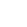
\includegraphics[width=20px]{figures/whitespace}
	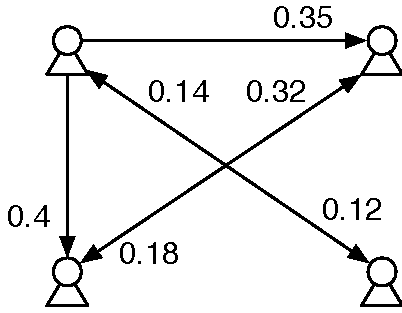
\includegraphics[width=0.38\columnwidth]{figures/coordRequirement}
	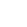
\includegraphics[width=20px]{figures/whitespace}
     \label{subfig:coordRequ}
  }
  \hspace{12pt}
  \subfigure[The actual coordination]{
    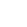
\includegraphics[width=20px]{figures/whitespace}
    \includegraphics[width=0.38\columnwidth]{figures/actualCoord}
    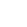
\includegraphics[width=20px]{figures/whitespace}
    \label{subfig:actualCoord}
  }
  \hspace{12pt}
  \subfigure[The coordination that is lacking]{
    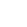
\includegraphics[width=20px]{figures/whitespace}
    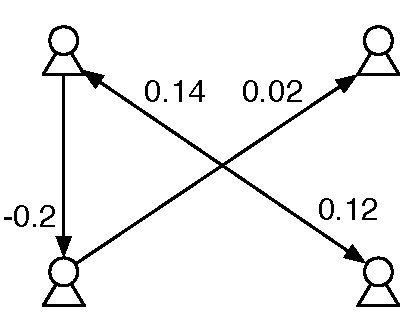
\includegraphics[width=0.38\columnwidth]{figures/coordLack}
    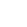
\includegraphics[width=20px]{figures/whitespace}
    \label{subfig:coordLack}
  }
	\caption{Comparing coordination needs with actual coordination to find lacking coordination}
	\label{fig:communication}
\end{figure*}

This measurement assigns a number between 0 and 1 to each entry in the task assignment, task-dependency, and actual coordination matrices.
The weighted assignment matrix is a $m\times n$ matrix where $m$ is the number of people and $n$ denotes the number of entities. 
Each entry in the matrix illustrates the strength of the connection between a person $i$ and an entity $j$. Such a connection may be the expertise person $i$ has with a task $j$, or the priority that person $i$ places on task $j$.

The weighted dependency matrix is an $n\times n$ matrix where $n$ denotes the number of entities.
Each entry in the matrix describes the strength of the relationship between two entities. The weighted dependency matrix may show the ratio of dependencies an entity has with another over the number of total dependencies that entity has on others. 
For example, an entity strongly coupled with another has a high entity dependency.

To calculate the coordination needs matrix, we use the same formula proposed by Cataldo, et al.~\cite{cataldo2006:coordination_reqs}, using the weighted values in the task assignment $A'$ and task dependency $D'$ matrices.

\[ CN' = A' \times D' \times (A')^t \]

\noindent This calculation will yield the weighted coordination needs matrix $CN'$, an $m\times m$ people by people matrix (Figure \ref{subfig:coordRequ}).
The coordination needs matrix shows how strong the relations between people are supposed to be based on their technical work.

\subsubsection{Weighted Actual Coordination}

Weighted actual coordination is a relative value that indicates the strength of a relationship between two individuals (Figure \ref{subfig:actualCoord}). A social network such as a communication network can be weighed according to the amount of ongoing communication. For example, one such weighing scheme may work as follows:

\begin{enumerate}
\item For a communication network, identify the largest value of communication between two individuals.
\item Divide all other values by the largest, thus normalizing the communication.
\item The result is a number between 0 and 1, where 1 indicates the largest value of communication in the network, and 0 is no communication.
\end{enumerate}

Other relationships that may be used as actual coordination are the amount of distance between individuals and how frequently they meet with other members in their team.

%\begin{comment}
%\subsection{Schemes for Weighing Actual Coordination}

%\begin{placeholder}
%\begin{itemize}
%\item Person--Artifact: Degree of assignment. The number of hours, proportionally, that someone is assigned to a task.
%\item Person--Artifact: The expertise a person has about a task, based on a known metric, such as the number of contributions made to a particular component of the software.
%\end{itemize}
%\label{box:weighted_congruence_schemes}
%\caption{Example Schemes for Weighted Congruence}
%\end{placeholder}

%Different actual coordination measurements may be used for the congruence calculation. We present a few examples of techniques that can be used to weigh actual coordination matrices:

%\textbf{Communication} A social network such as a communication network can be weighed according to the amount of ongoing communication. Consider Alice and Bob that work on dependent tasks:

%\begin{enumerate}
%	\item If Adam talks to Bart about his interdependent tasks, then for each task discussed the weight is increased by $a\cdot1/n$, where $a$ is the weight of the communication and $n$ is the number of Adam's tasks that depend on Bob's tasks.
%	\item In case Adam discusses a task dependency very frequently with Bart, then, given a three point scale ``occasionally/frequently/very frequently'', $a$ is set to 1. For another task that is only occasionally discussed, $a$ would be $0.\bar{3}$.
%\end{enumerate}
%In the end, if only two of Adam's tasks depend on Bart's tasks, the weight of Adam actual coordinating with Bart would be $1.0\cdot1/2+ 0.\bar{3}\cdot1/2= 0.6\bar{6}$.

%Another scheme is to scale the amount of communication to a value relative to the maximum number of comments in the network.
%\begin{enumerate}
%\item For a communication network, identify the largest value of communication between two individuals.
%\item Divide all other values by the largest one.
%\item The result is a number between 0 and 1, where 1 indicates the largest value of communication in the network, and 0 is no communication.
%\end{enumerate}

%\textbf{Distance}
%We can also measure the relationship between Alice and Bob by looking at different types of distance.
%We can measure:
%\begin{itemize}
%\item how far they are apart in terms of physical distance, like meters or kilometres,
%\item the time difference between their time zones, and
%\item the number of organizational units that part them.
%\end{itemize}
%These values are normalized to fit within 0 and 1. All three of those measures result in a symmetric matrix, meaning Alice will always have the same distance to Bart and vice versa.
%	
%After we weigh all entries within the task assignment, task dependency, and actual coordination matrix, we can compare the coordination requirements with the actual coordination using the method described in Section \ref{subsec:ourmeasure}.
%%We discuss next the expected benefits from this weighted approach.
%\end{comment}


%------------------------------------------------------------------------- 
\subsection{Identifying Gaps in Socio-Technical Congruence}
\label{sec:lack}

%Currently, there is no formal technique to identify which pairs of individuals have a gap in congruence.
We complement our
weighted congruence measure with a technique to generate a \emph{lack-of-coordination matrix}. This matrix not only identifies the
gaps between a coordination needs matrix and an actual coordination matrix, but can also identify the size of these gaps (Figure \ref{subfig:coordLack}). This lack-of-coordination matrix can be used with both unweighted congruence and weighted congruence.

% \[ g_{ij}(CN'_{ij}, AC'_{ij}) = \Big\lbrace \begin{array}{ l l } 1 \text{,}  & CN'_{ij} - AC'_{ij} > 0 \\ 0 \text{,} & \text{otherwise} \end{array} \]
 \[ g_{ij}(CN'_{ij}, AC'_{ij}) = CN'_{ij} - AC'_{ij} \]

\noindent for $i=1,\dots,m$ and $j=1,\dots,m$. The value of $g_{ij}$ is the \textbf{gap size} between the pair $ij$. The lack-of-coordination matrix illustrates situations where the proportion of communication exceeds the expected proportion of coordination needs. If the value is positive, then there is not enough coordination to satisfy the information needs requested by the $CN'$ matrix, resulting in a \textbf{gap}. If a value is negative, then there was more coordination than requested through the $CN'$ matrix, resulting in \textbf{overload}.  Neither situation necessarily results in a problem, but we believe that investigating overload and lack of coordination has implications on software engineering coordination.

% The values in this matrix may be normalized to create a relative distance between the coordination needs and communication. 

\subsection{Weighted Congruence Index}


To convert the lack-of-coordination matrix to a single socio-technical congruence measurement, we apply

\[ \text{congruence} = 1 - \frac{\displaystyle\sum^{m}_{i=1} \sum^{m}_{j=1} g_{ij}}{\displaystyle\sum^{m}_{i=1}\sum^{m}_{j=1}CN'_{ij}} \]
\noindent for each $i$ and each $j$, unless $i=j$. This value, which is usually between 0 and 1, is an overall level of the congruence in the current network. In theory, the formula allows the index to fall outside of this range for some edge cases, but we did not observe any such cases in practice.


\subsection{Benefits of Weighted Congruence}
\label{sec:benefit}

Using a weighted congruence model allows us to deal with situations that are not handled with unweighted congruence.
% We can investigate relationships between people and the technical entities in finer-grained detail, including situations where people have multiple coordination needs with others. 
Using the weighted congruence approach allows a person diagnosing the organization to benefit from \emph{locality} and \emph{relationship strength}.

\textbf{Locality}
allows us to identify which area of a network has a gap.
% Not only does this give us an overall measure of congruence, but now we can identify potential coordination problems in the network.
The lack-of-coordination matrix identifies which pairs of individuals do not fulfill coordination needs.
Although the original model does give us some limited locality in the sense of identifying congruence gaps, it is far more coarse grained.


%Using weighted congruence, we can identify people working on two interdependent tasks who do not discuss both technical entities.

\textbf{Relationship strength}
indicates how strong the relationship between two developers is. Relationship strength allows us to identify pairs of people who have multiple coordination needs, and therefore who need to coordinate more often with each other. Using relationship strength allows us to investigate coordination in more detail because we can investigate pairs with strong dependencies---these people also tend to be key individuals in a team.
\\

%ranks people pairs where more coordination might be needed by the computed lack of congruence.
%Ranking is a considerable improvement over Cataldo's model since it allows us to only extract an unordered list of gaps. 
%This also covers gaps, but does not necessarily priorates gaps more.
%Because filling congruence gaps can be risky~\cite{valetto2007:value,ehrlich2008:congruence_gaps}, a ranking can provides us with a better assessment of which gaps to fill first if at all.


\indent By allowing better locality and relationship strength, we believe that this weighted model provides an in-depth technique with which to study congruence.

%In the next section, we discuss how in our methodology we used these two
%measurements to investigate the relationship between socio-technical congruence
%and build success probability. 

\subsection{Comparison with Other Weighted Measures}

We know of three other methods for assigning a weight to relationships and gaps. Cataldo proposed a system using weights with integers \cite{cataldo2008:stc}. Ehrlich, et al. \cite{ehrlich2008:gaps} used a method to rank communication into three levels of importance. Gokpinar \cite{gokpinar2010} independently proposed a weighted congruence measure.

\subsubsection{Integer Matrices}

Cataldo's method assigns integer weights as values in the task assignment and task dependency matrices, resulting in a weighted coordination needs matrix. However, his formula in Section \ref{sec:stc} considers that a single communication instance is sufficient for satisfying any amount of coordination. Our method provides information about overload and lack of coordination, and provides a more fine-grained representation through the the lack-of-coordination matrix.

\subsubsection{Levels of Communication}

Ehrlich's method aggregates multiple relationships between two individuals to determine a ``level of communication''.  The relationships are: when two individuals work together on a project; when two individuals communicate several times a month for any reason; and when two individuals work together on shared files. If one or more of these relationships are true, they are added to provide a number representing the level.

% If one and only one of the above relationships hold between two individuals, then they are considered to be at level 1. If two of the relationships hold, then they are at level 2, and if all three relationships hold then they are at level 3. If none of the relationships hold, the connection between the two individuals is level 0, a gap.

The level of communication does not provide a ranking of gap size because they presume that a gap either exists, or that it is covered with one of the three levels. This paper mentions ranking gaps by size, but the gap rank is the total number of gaps that exist between two developers over the entire project. Thus, this measurement does not actually weigh the conceptual lack-of-communication distance between two individuals for each gap.
%Our proposed gap size measurement measure the size of a single gap.

\subsubsection{Coordination Deficit}

Gopkinar independently proposed a weighted congruence called ``coordination deficit'', which is equivalent to our gap size. It weighs the number of dependencies between components, and the number of communications between individuals. Like our method presented in prior work \cite{kwan2009:weighted}, they calculated the coordination deficit by normalizing the edges and subtracting the values between the equivalent of an actual coordination network and a coordination needs network. The fact that the authors used normalization and algebraic subtraction suggests that they are reasonable approaches to calculating gap size.



%--------------------------------------------------------------------------------------------------------------
\section{Research Methodology}
\label{sec:methodology}

In this section, we revisit our research questions, present our socio-technical
conceptualizations in RTC, and outline our analysis techniques.

\subsection{Research Questions}

%We are interested in using socio-technical congruence to study coordination in
%RTC. In particular, we are interested in investigating the effects of
%socio-technical congruence on build quality

%We have established that coordination is essential in software
%development, and that high socio-technical congruence, which is one measurement
%of coordination quality, corresponds to high developer productivity. We know
%that builds are relevant to the RTC team; in an interview with a RTC
%managers, he stated ``Build quality is almost code quality''.
%An ``OK'' build implies good software quality, and an ``error'' implies that mistakes have occurred during
%software development. The build success probability is the probability that a build will have an ``OK'' result.

\subsubsection*{Research Question 1: Does socio-technical congruence have an effect on build success probability in the RTC project?}

We hypothesize that high socio-technical congruence increases build success probability.

\subsubsection*{Research Question 2: Does gap size have an effect on build success probability in the RTC project?}

We hypothesize that the mean gap size in a build is inversely correlated with build success probability. That is, a smaller mean gap size is related to a larger probability of build success.

\subsection{Data Description and Collection}
\label{sec:data}

\begin{figure*}
  \setbox1=\hbox{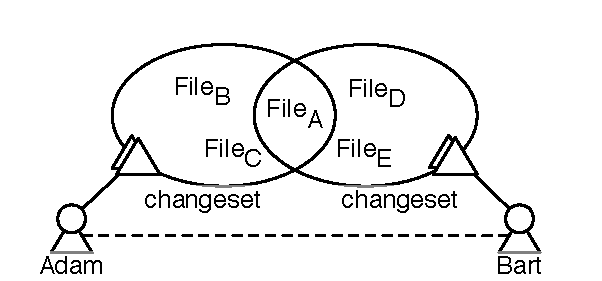
\includegraphics{figures/cochangedfiles}}% The smaller image
  \setbox2=\hbox{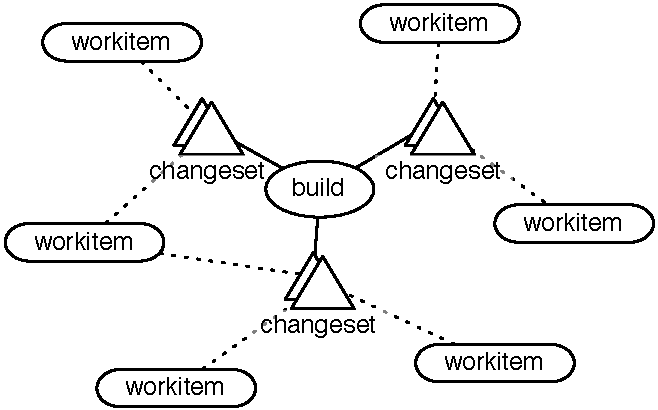
\includegraphics{figures/buildworkitem}}% The larger image 
	
  \centering
  \subfigure[Relationship among Builds, Change Sets, Files, and Work Items]{
    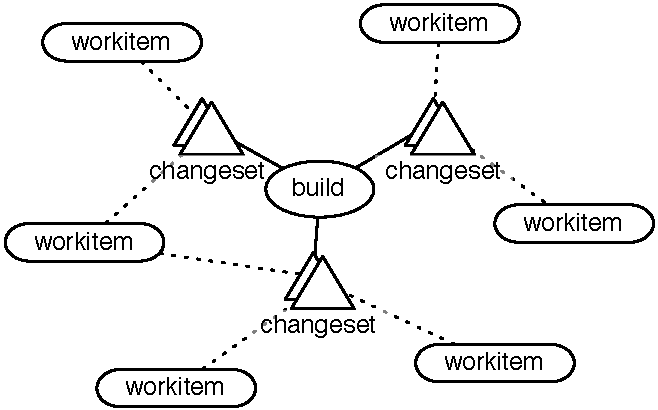
\includegraphics[scale=0.5]{figures/buildworkitem}
    \label{fig:buildworkitem}
  }
  \hspace{8pt}
  \subfigure[Constructing a Coordination Needs Instance]{
  	\raisebox{0.4\ht2-0.5\ht1}{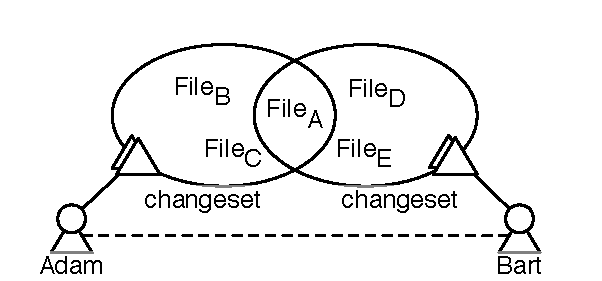
\includegraphics[scale=0.5]{figures/cochangedfiles}} \hfill
    \label{fig:cochangedfiles}
  }
  \hspace{8pt}
  \subfigure[Constructing an Actual Coordination Instance]{
	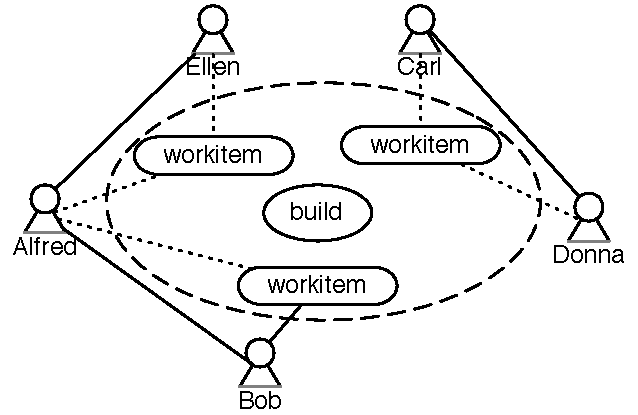
\includegraphics[scale=0.5]{figures/buildsn}
     \label{fig:buildsn}
  }
  \caption{Conceptualizing Socio-technical Congruence in IBM Rational Team Concert}
  \label{fig:constructing}
\end{figure*}

In collaboration with IBM, we acquired a copy of the RTC repository containing data over a one year period.
%between June 2007 and June 2008.
This period of time covers twelve ``milestones'', varying from 1 week to 4 weeks long, during which the RTC team achieved a number of objectives. The end of our data set coincides with a major milestone in which RTC was to be released for open beta testing. 

In addition to quantitative data, we had obtained contextual information about the development team. We also investigated work items, comments, and reports available on the \texttt{jazz.net} web site.

The repository contains build information, work items, comments, change sets, and anonymised author information. We describe the data in more detail below.

\textbf{Work item.} A work item is a description of a unit of work to be done. A work item can be assigned a type of \emph{task}, \emph{enhancement}, or \emph{defect}.
We extracted 2008 unique work items that were relevant to our study.
The same work item may be involved in multiple builds; a total of 9218 non-unique work items were associated with a build across our data set. As our conceptualization focuses on the per-build level, we must consider these non-unique work items.

\textbf{Build.} A build is the process of compiling the software to create a working program.
A build outcome can be an \emph{error}, which indicates that there was either a
compilation error or a test suite error, \emph{OK}, which indicates no
errors, and \emph{Warning}, which indicates that there were warnings
returned by the compiler or the test suites.

A build contains the work from one or more work items, and these work items are not necessarily unique from build to build. The RTC repository does not keep a full record of every build over time, which means that we have more data points for the two most recent milestones compared to earlier in the project.

The RTC repository contains 533 builds, but we consider only builds that contain coordination needs, therefore dropping the number of builds to 214.  We remove 17 builds whose result is Warning because the way that the RTC team treats its Warning builds is dependent on the build. Finally, we remove 7 builds whose types could not be identified. The resulting data set contains 191 builds.

There are three types of builds that we investigate in this study: \emph{continuous builds}, \emph{nightly builds}, and \emph{integration builds}. Continuous builds, which are run regularly by a user, incorporate changes from the local development site, plus known stable components from remote sites.  Nightly builds also incorporate changes from the local site and stable components from remote sites approximately once a day. Integration builds integrate the latest components from every development site. The integration builds are often expected to break due to their large complexity, but errors in continuous and nightly builds are potentially indicative of coordination problems. Our data contains 122 continuous builds, 55 nightly builds, and 14 integration builds.

Because we have a data set of builds over time, we include the date of a build as a variable in our analysis. The build date is conceptualized as the number of days after the first build in our data set.

\textbf{Comment.} A comment is written text authored by a developer that is about a particular work item. Comments are the primary method of transferring information among developers in RTC. Multiple comments may be attached to a single work item. The data subset contains 9323 comments.
%Comments are not threaded---that is, we do not know if a comment specifically references an existing comment in the work item discussion. \\

\textbf{Change set.} A change set is a collection of code changes to a number of files. When a developer updates the repository, all of the files that were changed together are updated in a single change set. A change set is generated by one author only, and is related to exactly one work item. A single work item may contain multiple change sets, and the same change set may occur in multiple builds. There are 3013 change sets in RTC. The number of change sets per work item ranges from 1 to 246. Ninety-five percent of the work items contain 15 or less change sets, and 42\% of the work items contain only one change set.

\textbf{Source code file.} A file contains source code and is included in change sets. Over time, a file may be associated with multiple change sets.

\textbf{Author.} An author is someone who has contributed to RTC. In our conceptualization, we specifically identify an author as meaning someone who has submitted a change set containing modifications to files. Because each change set can be attributed to one author, there are always at least as many change sets as there are authors in a build.


\subsubsection{Distribution of Build Data}

% We illustrate the authors, change sets, work items, and files per build in Figure \ref{fig:buildworkitem}.

Each build involves a number of file authors, change sets, work items, and files. The same author, file, and work item may be involved across multiple builds.
We plot the histograms for each of these entities in Figures \ref{fig:hist_authors}, \ref{fig:hist_changesets}, \ref{fig:hist_workitems}, and \ref{fig:hist_files}.
Most of these distributions, especially the files, are skewed toward the left. 

%We show a scatterplot of the relationships between the number of authors and the number of files per build, as well as the number of authors and the number of work items per build. There is a correlation between authors and files (Spearman $\rho = 0.78$) and no correlation between the number of authors and the number of work items per build (Spearman $\rho=0.056$).

% -------------------------- MOVED TO APPENDIX -------
\begin{figure*}[ht]
\centering

	\subfigure[Authors per Build] {
		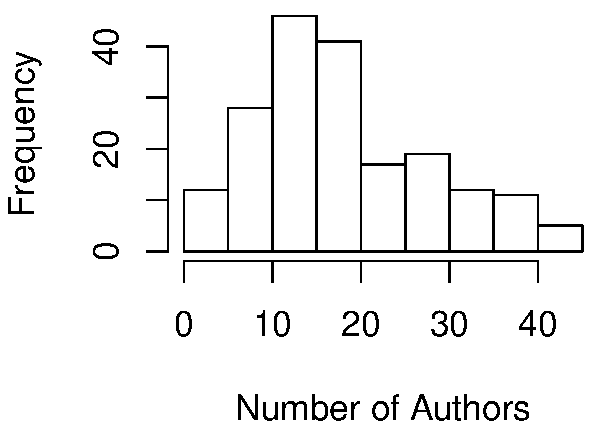
\includegraphics[scale=0.372]{figures/hist_authors_per_build}
		\label{fig:hist_authors}
	}
	\subfigure[Change Sets Per Build] {
		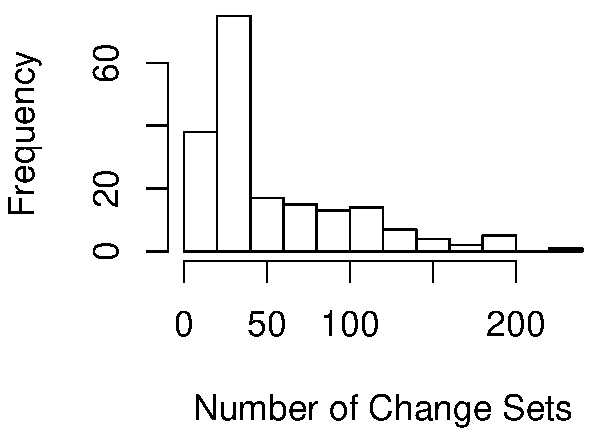
\includegraphics[scale=0.372]{figures/hist_changesets_per_build}
		\label{fig:hist_changesets}
	}
	\subfigure[Work Items Per Build] {
		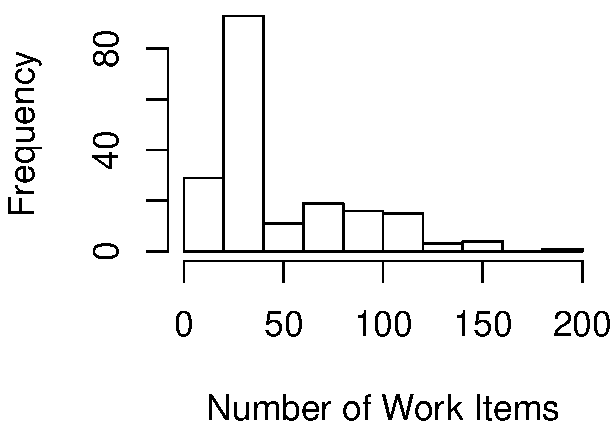
\includegraphics[scale=0.372]{figures/hist_workitems_per_build}
		\label{fig:hist_workitems}
	}	
	\subfigure[Files Per Build] {
		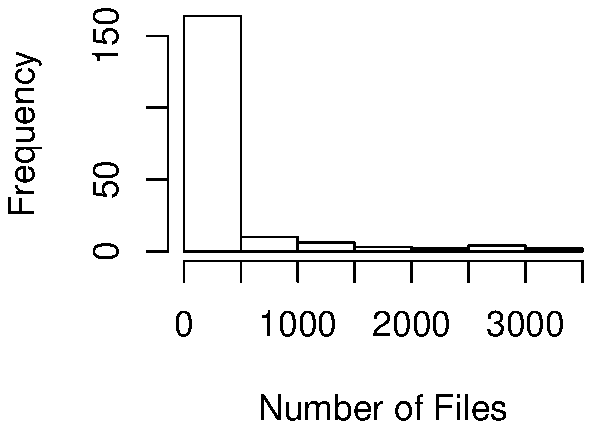
\includegraphics[scale=0.372]{figures/hist_files_per_build}
		\label{fig:hist_files}
	}
	\caption{Distribution of authors, change sets, work items, and files per build}
	\label{fig:entities_per_build}

\end{figure*}
% -------------------------- MOVED TO APPENDIX -------

%\begin{figure}
%\centering
%
%	\subfigure[Authors vs Files] {
%		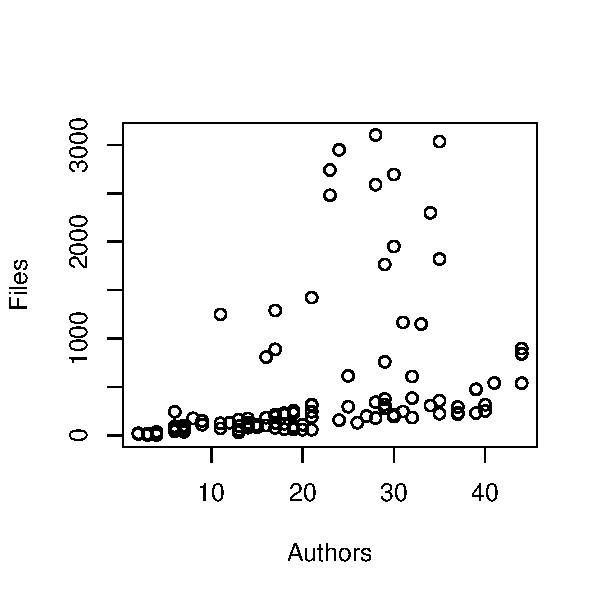
\includegraphics[scale=0.4]{figures/scatter_authors_files}
%		\label{fig:scatter_authors_files}
%	}
%	\subfigure[Authors vs Work Items] {
%		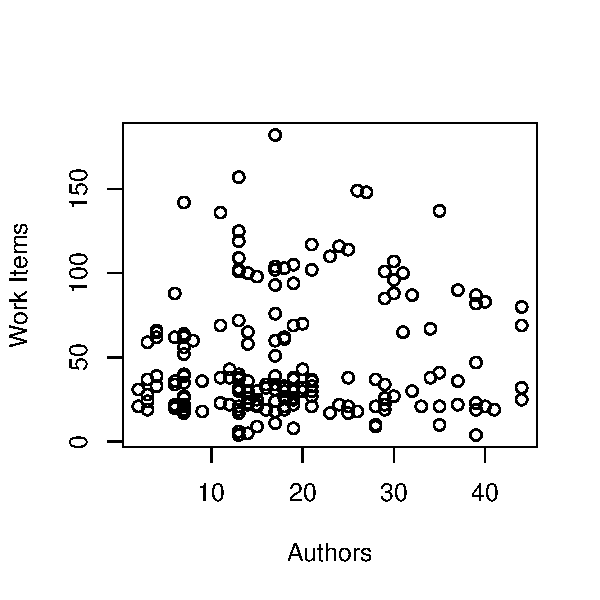
\includegraphics[scale=0.4]{figures/scatter_authors_workitems}
%		\label{fig:scatter_authors_workitems}
%	}
%	\caption{Relationship between build variables per build}
%	\label{fig:relationship_builds}
%\end{figure}

\subsection{Analysis Method}
\label{sec:analysis}

We use the unweighted congruence measure and weighted congruence measure presented in Section \ref{sec:congruence} for our analysis. We explain how we conceptualize congruence in this section.

\subsubsection{Conceptualizing Coordination Needs}

% We conceptualize technical dependencies as files that were changed together in multiple change sets in a build.

Previous studies use various heuristics for determining the dependencies between modules. One conceptualization is based on method call graphs generated by static code analysis, and has been used by Ehrlich \cite{ehrlich2008:gaps}.  Another conceptualization is a ``files-changed together'' heuristic, used by Cataldo \cite{cataldo2006:coordination_reqs}, where the files that were modified in the solution of a change request are considered to be dependent on each other. A third conceptualization is to use experts who manually identify dependencies~\cite{gokpinar2010}.

We decided to construct dependencies based on a variation of the files-changed together heuristic because a ``files-changed together'' heuristic was more reflective of social relationships than a call-graph approach \cite{cataldo2008:stc}, and best reflected our understanding of the RTC team's work.

We presume that a coordination need between two individuals exists if, minimally, these two individuals change the same file within the same build. In RTC, since only one author can be associated with each file check-in, there are two change sets involved, one associated with each file author. These two individuals should communicate with each other to ensure that the appropriate file dependencies are properly handled before the software is built (Figure \ref{fig:cochangedfiles}).

We generate the coordination needs matrix as follows.

\textbf{1) For each build, we identify every change set included in the build.} Every change set between the previous build and the current build is considered a part of the current build.

\textbf{2) We determine authorship for each file to generate the assignment matrix \emph{A}.} Since each change set has only one author, the author is assigned to every file in that change set. If an author modifies the same file in a different change set, then we add an additional edge for each change set in which the author changed that file.

\textbf{3) We determine the file dependencies in a build to generate the dependency matrix \emph{D}.} We iterate through every change set in the build. Each file is dependent on every other file within a change set. For example, if there are two change sets $C_1$ and $C_2$ in Build 1, with $C_1$ containing files A, B, and C, and $C_2$ containing files A, D, and E, the resulting dependency matrix $D$ would correspond to Figure \ref{fig:cochangedfiles}. In weighted congruence, we add one additional edge for each file pair that exists in each additional change set in that build. Thus, in a Build 2 with change sets $C_3$=\{A,~B,~C\} and $C_4$=\{A,~B\}, the dependency matrix entries in $D$ would be $D_{AB}= 2$, $D_{AC}=1$, and $D_{BC}=1$.

\textbf{4) We calculate the coordination needs as per the coordination needs calculation in Section \ref{sec:stc}.} The diagonals are ignored. When applying weighted congruence, we normalize the coordination needs matrix by taking the highest-ranked edge and dividing every entry in the matrix by that value. This converts each edge to a value between 0 and 1, indicating the relative rank of a coordination need between two individuals in the matrix.

We use this conceptualization because of the explicit relationships between change sets, builds, and authors in RTC. In previous ``files-changed-together'' approaches, multiple files checked in together were associated with multiple authors, whereas in RTC, a change set is authored by one author only. Our conceptualization of coordination needs represents a situation in which two individuals work on a file that are in two different change sets, but are within the same build. Though the file-level changes may not necessarily be to the same lines of code, we presume that multiple changes within a single file are sensitive enough such that each developer working on that file benefits by being informed of every change.

\subsubsection{Conceptualizing Actual Coordination}


We conceptualize actual coordination as communication through comments in the
RTC environment. We treat those who comment on a work item as a group of communicators, and assign weights when individuals comment on multiple work items that others also comment on (Figure \ref{fig:buildsn}).

Though the RTC commenting system allows users to post multiple posts to the same work item, we do not count multiple posts in a single work item as weighted communication.
Since a work item comment can be read by anyone with access to the work item repository, and there is no threading in the work item comments, we cannot assume that there is point-to-point communication from one person directly to another.
In addition, comment communication within the same work item do not correspond to weighted technical dependencies that cross different change sets.

We calculate the actual coordination matrix as follows.

\textbf{1) We identify the comments from the work items involved in a build.} Each build contains a number of change sets, and each change set has an associated work item with comments. For each work item, we include every comment that was posted after the previous build, but before the current build started.

\textbf{2) For each person who commented on a work item, we add a communication edge to every other person who commented on the same work item.} In weighted congruence, add one additional communication edge for each additional work item in which two individuals comment. We do not count weights for multiple comments in a single work item for the reasons discussed above. Thus, if work item $W_1$ contains commenters {A, B, C} and $W_2$ contains {B, C, D}, the resulting entries in the actual coordination matrix $AC$ would be $AC_{AB}=1$, $AC_{BC}=2$, $AC_{CD}=1$, $AC_{AC}=1$, and $AC_{CD}=1$.

\textbf{3) When applying weighted congruence, we normalize the communication network by taking the highest-ranked edge and dividing every edge in the network by that value.} This converts each edge to a value between 0 and 1, indicating the relative rank of comment-based communication between two individuals in the network.

This conceptualization of weighted communication represents the number of people who post a comment to the same work item.

We considered incorporating the RTC development mailing list into communication, but inspection of the mailing list revealed that the developers did not talk about technical issues and that the development list is primarily used for general announcements.

Unfortunately, due to the distribution of the 151 developers in the RTC team, as well as the one-year time period across which our study is conducted, we were unable to collect communication data such as instant messenger or face-to-face communication that we could associate to individual builds. Our concern with this missing data led us to inquire about the use of other forms of media among the team. We learned that although unofficial communication does happen between developers, the RTC team culture requires that the content of unrecorded and private communications be recreated as work item comments for consumption by remote project participants. We still expect that socio-technical congruence will be lower than we might expect from such a team as a consequence.

\subsubsection{Conceptualizing Gap Size}

The gap size in RTC represents a relative distance between the coordination needs and actual coordination. Since the two measurements are not necessarily comparable to each other, we normalize both measures to identify a relative ``rank'' of coordination needs and actual coordination. For example, if there is a coordination need in a build that has many dependencies, intuitively we would want a larger amount of communication around that build rather than on a build with few coordination needs. The gap size calculation identifies this mismatch.

We use the weighted congruence measure to compute the gap size. For each build, we calculate the gap size between each pair with a coordination need using the lack-of-coordination matrix explained in Section \ref{sec:lack}. Because of the normalization, each gap size is a value from $1$ to $-1$, where 1 is a large gap with little or no communication, 0 is full congruence, and -1 is a gap where there is more communication than necessary to fulfill the coordination need. We take the mean of these gap sizes and use this as a variable in a logistic regression model. We also consider an alternative calculation of gap size where we do not punish extra communication and set all values of gap size less than 0 to 0.

\subsubsection{Statistical Analysis Methods}

%Most of our data is highly skewed to the left, meaning that we have a larger proportion of small values than we would expect from a normal distribution. We attempted to fit the data to a log approximation, but found that even with this transformation, the Kolmogorov-Smirnov Test showed significant differences between a normal distribution and our data for both unweighted and weighted congruence. To account for this we use non-parametric statistics to test significance between variables.

To answer Research Question 1, we conceptualize congruence as described in Section \ref{sec:analysis} and test our hypothesis using logistic regression.

Logistic regression is ideal to test the relationship between multiple variables and a binary outcome, which in our study is a build result being either ``OK'' or ``Error''. The presence of many data entities in this project means that we must consider confounding variables in addition to the socio-technical congruence when determining its effects on the probability of build success. Informally, logistic regression identifies the amount of ``influence'' that a variable has in the probability that a build will be successful.

We show the relationship between a variable and the build success probability by plotting the y-axis as the probability. We use probability because we feel that it is more intuitive than odds ratios or logistic functions. If there is a relationship between a variable and the probability of build success, then we should see that as the variable's value increases, the probability also increases. In the probability figures, the solid line is the expected value, and the dashed lines indicate the 95\% confidence intervals.

We run two different logistic regression models: one using weighted congruence, and one using unweighted congruence. We include the following variables: number of files per build, number of authors contributing to the build, number of files in the build, number of work items per build, the congruence, the build type, and the date of the build. We centre and scale each numeric variable.
Because we were concerned about possible interactions affecting our results, we included first-order interaction effects and used backward stepwise elimination to remove variables to keep AIC (Akaike's Information Criterion) low.


% We include also every first-order interaction between these variables to test for possible interaction effects. % Including these interaction effects increased the reliability of the regression model.
%% FIX?
%, increasing the model likelihood ratio $\chi^2$ from 40.04 to 67.15 in the unweighted case $(p = 0)$ and 39.13 to 58.08 in the weighted case $(p = 0)$.

To answer Research Question 2, we calculate the gap size and include this as a variable in our logistic regression model to study the effects on build success probability.

% To answer Research Question 3, we examine in detail overall characteristics of RTC to explore other potential influences that may affect congruence, as well as build results. Data that we examine include the effect of other variables on the build success probability, and the effects of social factors on congruence, such as communication and commenting behaviour.

We use R \cite{R} and the Design package \cite{designR} for logistic regression analysis.

%--------------------------------------------------------------------------------------------------------------


\section{Results}
\label{sec:results}

In the RTC repository, we analysed 191 builds; of these builds, 60 were error builds, and 131 were OK builds. Table \ref{tab:summary} displays summary statistics per build.
Figure \ref{fig:hist_unweighted_congruence} displays histograms for unweighted congruence, and Figure \ref{fig:hist_weighted_congruence} shows histograms for weighted congruence. The histograms compare the frequencies for each type of congruence for all builds, the OK builds, and the error builds only. There are some minor differences between unweighted and weighted congruence values; weighted congruence, for instance, largely reduces the number of ``fully'' congruent situations where congruence is 1.

% % latex table generated in R 2.11.0 by xtable 1.5-6 package
% Wed Jul 14 23:11:04 2010
\begin{table}[ht]
\begin{center}
\begin{tabular}{rrrrr}
  \hline
 & VIF & Tol & VIF & Tol \\ 
  \hline
authors & 2.31 & 0.43 & 1.26 & 0.80 \\ 
  changesets & 2.27 & 0.44 & - & - \\ 
  files & 1.16 & 0.87 & 1.15 & 0.87 \\ 
  workitems & 1.03 & 0.97 & 1.03 & 0.97 \\ 
  type=I & 1.15 & 0.87 & 1.16 & 0.86 \\ 
  type=N & 1.05 & 0.96 & 1.04 & 0.96 \\ 
  unweightedCong & 1.19 & 0.84 & 1.15 & 0.87 \\ 
   \hline
\end{tabular}
\caption{Collinearity involving Unweighted Congruence}
\label{tab:vif-unweighted}
\end{center}
\end{table}

% % latex table generated in R 2.11.0 by xtable 1.5-6 package
% Wed Jul 14 23:11:04 2010
\begin{table}[ht]
\begin{center}
\begin{tabular}{rrrrr}
  \hline
 & VIF & Tol & VIF & Tol \\ 
  \hline
authors & 2.45 & 0.41 & 1.29 & 0.77 \\ 
  changesets & 2.25 & 0.44 & - & - \\ 
  files & 1.16 & 0.86 & 1.14 & 0.87 \\ 
  workitems & 1.01 & 0.99 & 1.01 & 0.99 \\ 
  type=I & 1.08 & 0.92 & 1.09 & 0.92 \\ 
  type=N & 1.05 & 0.95 & 1.04 & 0.96 \\ 
  weightedCong & 1.12 & 0.89 & 1.11 & 0.90 \\ 
   \hline
\end{tabular}
\caption{Collinearity involving Weighted Congruence}
\label{tab:vif-weighted}
\end{center}
\end{table}


The congruence values are low on average. The unweighted congruence has a mean value of 0.331, and the weighted measure has a mean value of 0.196, meaning that about one-third and one-fifth of the coordination needs are satisfied by actual coordination, respectively. Over 75\% of the builds have a weighted congruence value of less than 0.25.

\begin{figure}[t]
  \centering
  \subfigure[All builds]{
    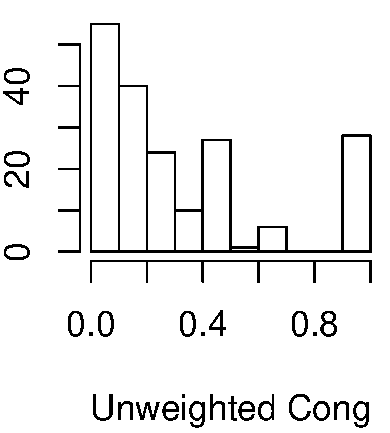
\includegraphics[scale=0.372]{figures/hist_unweighted}
    \label{subfig:hist_nonweighted}
  }
    \subfigure[OK builds]{
    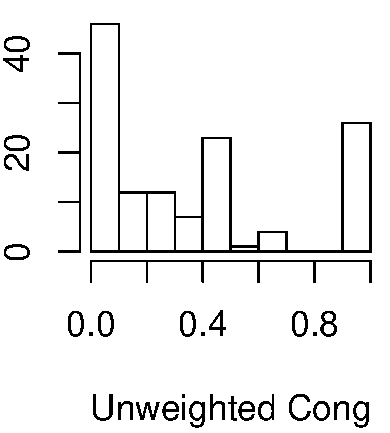
\includegraphics[scale=0.372]{figures/hist_unweighted_ok}
    \label{subfig:hist_nonweighted_ok}
  }
  \subfigure[Error builds]{
	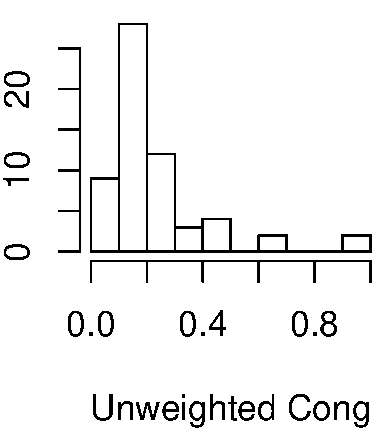
\includegraphics[scale=0.372]{figures/hist_unweighted_err}
     \label{subfig:hist_weighted_err}
  }
	\caption{Distribution of Unweighted Congruence Values}
	\label{fig:hist_unweighted_congruence}
\end{figure}

\begin{figure}[t]
  \centering  
  \subfigure[All builds]{
	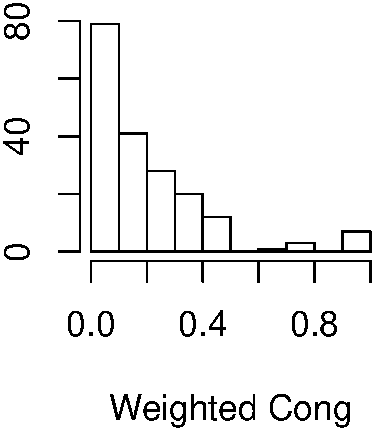
\includegraphics[scale=0.372]{figures/hist_weighted}
     \label{subfig:hist_weighted}
  }
  \subfigure[OK builds]{
    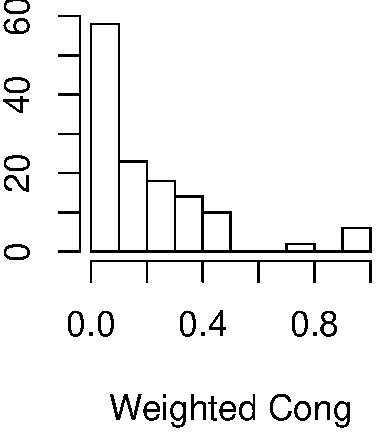
\includegraphics[scale=0.372]{figures/hist_weighted_ok}
    \label{subfig:hist_nonweighted_ok}
  }
  \subfigure[Error builds]{
	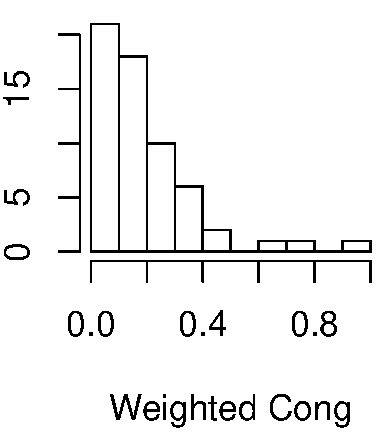
\includegraphics[scale=0.372]{figures/hist_weighted_err}
     \label{subfig:hist_weighted_err}
  }
	\caption{Distribution of Weighted Congruence Values}
	\label{fig:hist_weighted_congruence}
\end{figure}

%              weighted  unweighted     authors       files  workitems        date
%weighted    1.00000000  0.77321937 -0.22499546 -0.13734420 0.04553513  0.02475572
%unweighted  0.77321937  1.00000000 -0.26675774 -0.21972887 0.08265125  0.19178548
%authors    -0.22499546 -0.26675774  1.00000000  0.41240536 0.09800938 -0.30061898
%files      -0.13734420 -0.21972887  0.41240536  1.00000000 0.07767137 -0.20237118
%workitems   0.04553513  0.08265125  0.09800938  0.07767137 1.00000000  0.03615854
%date        0.02475572  0.19178548 -0.30061898 -0.20237118 0.03615854  1.00000000


%We examined data for multicollinearity using variance inflation factor (VIF)~\cite{davis1986}.
%%A high VIF value suggests multicollinearity may exist among the variables, and a low VIF value suggests a lack of multicollinearity.
%% We create separate models for unweighted congruence (Table \ref{tab:vif-unweighted}) and weighted congruence (Table \ref{tab:vif-weighted}).
%In both weighted and unweighted congruence models, there is a significant risk of multicollinearity between authors and change sets.
%We choose to remove change sets from our models because, due to the enforced processes in RTC, we know that there is exactly one author per change set, and therefore, in a build, there is always at least as many change sets as authors, and that removing change sets has no bearing on dependencies as dependencies are calculated at the file level.
%% Removing the change sets reduces the multicollinearity risk.

%Recalculating the VIF indicates that the values are reduced in line with the other variables.
% Model II in Tables \ref{tab:vif-unweighted} and \ref{tab:vif-weighted} illustrate the model without change sets, and shows a reduced risk of multicollinearity between the remaining variables.
% Consequently, the logistic regression models in the remainder of this paper do not include change sets as a variable.

\begin{table}[t]
\centering

\begin{tabular}{l|rrrr}


 & Min & Median & Max & Mean\\\hline
Authors & 2 & 17 & 44 & 18.62\\
Files & 5 & 131 & 3101 & 342.3 \\
Change Sets & 4  & 34  & 226 & 54.2\\
Work items & 4 & 34  & 182 & 48.3 \\
Build date range (days) & 0  & 345  & 361 & 319.2 \\
Unweighted cong. & 0  & 0.21  & 1 & 0.331 \\
Weighted cong. & 0 & 0.15  & 1 & 0.196\\
Gap size & -0.083 & 0.190 & 1.00 & 0.317 \\
\hline
\end{tabular}

\caption{Summary statistics}
\label{tab:summary}
\end{table}

\begin{table}[t]
\begin{center}
\begin{tabular}{l|rrrrrr}


 & 2. & 3. & 4. & 5. & 6. & 7. \\ 
  \hline
   1. Weighted & 0.77 & -0.22 & -0.14 & -0.12 & 0.05 & 0.02 \\ 
   2. Unweighted  &-- & -0.27 & -0.22 & -0.33 & 0.08 & 0.19 \\ 
   3. Authors &  & --& 0.41 & 0.76 & 0.10 & -0.30 \\ 
   4. Files &  &  & --& 0.37 & 0.08 & -0.20 \\ 
   5. Change sets &  &  &  &  --& 0.02 & -0.38 \\ 
   6. Work items  &  &  &  &  &  --& 0.04 \\ 
   7. Build date &  &  &  &  &  & -- \\ 
\hline

\end{tabular}
\end{center}
\caption{Pairwise Correlation of Variables per Build}
\label{tab:pairwise}
\end{table}

We calculated pairwise correlations between the variables weighted congruence, unweighted congruence, number of authors, number of files, number of change sets, number of work items, and build date (Table \ref{tab:pairwise}). There is a strong correlation between weighted and unweighted congruence, which is expected; a strong correlation between change sets and authors; and a weak correlation between authors and files. To avoid multicollinearity problems in our data, we choose to remove change sets from our logistic regression analysis because, due to the enforced processes in RTC, we know that there is exactly one author per change set, and thus there is at least as many change sets as authors per build. Note that weighted congruence and unweighted congruence do not appear in the same model and are thus not subject to multicollinearity problems.

To assess the fit of the logistic regression models, we use the Nagelkerke pseudo-$R^2$ and AIC. $R^2$ shows the proportion of variability explained by the model, and AIC is a measure of how well the model fits the data. Ideally, $R^2$ is high and AIC is low. Our current model contains 19 variables and has an $R^2$ of 0.581 and 0.548 for unweighted and weighted congruence models respectively. We compared our model in Table \ref{tab:models} to a model containing every first-order interaction effect with 27 variables and a model that contains the 7 main effects only (in Table \ref{tab:logr_maineffects}). We found that 19 variables is optimal and that removing further variables lowered the $R^2$ value while raising the AIC.

We observe also that the unweighted congruence model and the weighted congruence model are very similar, with a difference in Nagelkerke $R^2$ of only 0.030.

\begin{table}
\begin{center}
\begin{tabular}{l|r|rr|rr}

             & & \multicolumn{2}{c|}{Unweighted} & \multicolumn{2}{c}{Weighted} \\
Model                  & Variables    & AIC & $R^2$                       & AIC & $R^2$                      \\ \hline
Every interaction  & 27  & 188.6 & 0.595 & 196.7 & 0.559 \\
Main effects only & 7   & 213.2 & 0.269 & 214.2 & 0.263 \\
\textbf{Our model}         & \textbf{19}  & \textbf{175.8} & \textbf{0.581} & \textbf{183.4} & \textbf{0.548} \\
\hline
\end{tabular}
\end{center}
\caption{Model comparison}
\label{tab:models}
\end{table}



% To assist with evaluating the fit of our models, we compared the logistic regression models with the main effects only to the models that included the interaction effects. To evaluate their performance, we used bootstrapping \cite{harrell2001} for each model and plot the results of  the predicted model versus the actual results (Figures \ref{fig:calibrate}). \texttt{Appa}, which stands for apparent validity, provides an optimistic estimate of model performance, and \texttt{bias-corrected} indicates a non-parametric calibration curve estimated from the predicted values. \texttt{Ideal} indicates that the predicted model fits the actual data. We observe that the models with main effects must correct strongly for bias and do not fit as well as the model that includes interaction effects.






% latex table generated in R 2.11.0 by xtable 1.5-6 package
% Thu Jul 29 14:02:07 2010



\subsection{Effects of Congruence on Build Result}
\label{sec:congruence_effect_build_result}


\begin{table*}
\begin{center}
\begin{tabular}{l|rrr|rrr}
 & \multicolumn{3}{c|}{Unweighted} & \multicolumn{3}{c}{Weighted} \\\hline
Variable & Coef. & S.E. & \emph{p} & Coef. & S.E. & \emph{p} \\
	\hline
Intercept                   &  -0.5459 &   0.4663 & 0.2417 &    0.3289 &    0.4729 &   0.4867 \\
\textbf{Congruence}              &   \textbf{6.3410} &   \textbf{1.6262} & \textbf{**0.0001} &    3.6699 &    2.3013 &   0.1108 \\
\textbf{Authors}                     &  \textbf{-1.9759} &   \textbf{0.5310} & \textbf{**0.0002} &   \textbf{-2.0176} &    \textbf{0.5802} &   \textbf{**0.0005} \\
\textbf{Files}                       &  \textbf{-1.0734} &   \textbf{0.4561} & \textbf{*0.0186} &   \textbf{-1.1169} &    \textbf{0.5099} &   \textbf{*0.0285} \\
Work~items                   &  -0.1456 &   0.2355 & 0.5363 &   -0.1365 &    0.2343 &   0.5602 \\
\textbf{Build type=I}                      &   \textbf{2.1533} &   \textbf{1.0526} & \textbf{*0.0408} &    1.2777 &    1.0172 &   0.2091 \\
Build type=N                      &   4.6833 & 200.7587 & 0.9814 &    2.7593 &  192.5236 &   0.9886 \\
Build date                   &  -0.6560 &   0.6709 & 0.3282 &   -0.1352 &    0.7133 &   0.8497 \\
\textbf{Congruence * Build type=I}     &  \textbf{-9.2151} &   \textbf{2.5572} & \textbf{**0.0003} &   \textbf{-6.2748} &    \textbf{2.9664} &   \textbf{*0.0344} \\
Congruence * Build type=N     &  -7.7308 &  91.8053 & 0.9329 &   -7.2024 &  188.1811 &   0.9695 \\
Congruence * Build date  &  \textbf{-5.1266} &   \textbf{1.9290} & \textbf{**0.0079} &   \textbf{-5.5670} &    \textbf{1.9760} &   \textbf{**0.0048} \\
Authors * Build type=I            &   1.2688 &   0.7028 & 0.0710 &    1.1852 &    0.7370 &   0.1078 \\
Authors * Build type=N            & 105.4123 & 535.8792 & 0.8441 &  103.0155 &  521.0808 &   0.8433 \\
Authors * Build date         &  -0.6061 &   0.3616 & 0.0937 &   -0.6004 &    0.3576 &   0.0932 \\
Authors * Files             &   0.7663 &   0.4289 & 0.0740 &    0.4979 &    0.5232 &   0.3414 \\
Files * Build type=I              &   1.0920 &   1.1838 & 0.3563 &    1.7042 &    1.4099 &   0.2267 \\
Files * Build type=N              & -37.9274 & 199.2314 & 0.8490 &  -36.5156 &  192.3382 &   0.8494 \\
\textbf{Work~items * Build date}       &   \textbf{0.8040} &   \textbf{0.3003} & \textbf{**0.0074} &    \textbf{0.8909} &    \textbf{0.3466} &   \textbf{*0.0102} \\
\textbf{Build type=I * Build date}          &   \textbf{2.6442} &   \textbf{0.7678} & \textbf{*0.0006} &    \textbf{1.8627} &    \textbf{0.7621} &   \textbf{*0.0145} \\
Build type=N * Build date          &  84.7252 & 344.8129 & 0.8059 &   84.3117 &  341.4988 &   0.8050 \\
	\hline
Model likelihood ratio & 101.92 & $p \approx 0$ & $R^2=0.581$ & 94.36 & $p \approx 0$ &	$R^2 = 0.548$ \\
& \multicolumn{3}{c}{191 observations} & \multicolumn{3}{c}{191 observations} \\
\multicolumn{1}{l}{ } & \multicolumn{6}{l}{\scriptsize{Build type is set to continuous}} \\
\multicolumn{1}{l}{\scriptsize{*$p < 0.05$; **$p < 0.01$}} & \multicolumn{6}{l}{\scriptsize{Nagelkerke is used as the pseudo-$R^2$ measure}}
\end{tabular}
\end{center}
\caption{Logistic Regression models predicting build success probability with main and interaction effects}
\label{tab:logr}
\end{table*}

%\begin{table*}
\begin{center}
\begin{tabular}{lrrrrrr}
Variable & Coefficient & S.E. & Wald Z & p Value & Odds Ratio & 95\% CI \\
	\hline
Intercept                  &  2.666e+00  & 1.150e+00  &  2.32   & 0.0205 & - & - \\
authors                    & -6.173e-02  & 5.627e-02  & -1.10   & 0.2726 & 9.401361e-01 & 0.11 -- 6.100000e-01    \\
files                      & -7.955e-03  & 3.571e-03  & -2.23   & 0.0259 & 9.920763e-01 & 0.43 -- 8.500000e-01    \\
workitems                  & -1.329e-03  & 1.978e-02  & -0.07   & 0.9464 & 9.986723e-01 & 0.35 -- 1.580000e+00    \\
type=I                     &  2.654e-01  & 1.371e+00  &  0.19   & 0.8465 & 1.303928e+00 & 1.15 -- 7.580000e+00    \\
type=N                     & -3.727e+01  & 2.230e+01  & -1.67   & 0.0947 & 6.481571e-17 & 0.18 -- 2.020000e+00    \\
unweightedCong             &  5.702e+00  & 3.405e+00  &  1.67   & 0.0940 & 2.993381e+02 & 0.06 -- 8.016193e+10    \\
\hline
authors * files            &  1.651e-04  & 7.361e-05  &  2.24   & **0.0249 &              &  \\
authors * workitems        & -4.685e-04  & 6.799e-04  & -0.69   & 0.4908 &              &  \\
authors * type=I           &  2.087e-02  & 4.738e-02  &  0.44   & 0.6596 &              &  \\
authors * type=N           &  3.034e+00  & 1.813e+00  &  1.67   & 0.0942 &              &  \\
authors * unweightedCong   & -2.738e-01  & 2.015e-01  & -1.36   & 0.1741 &              &  \\
files * workitems          &  7.790e-06  & 9.971e-06  &  0.78   & 0.4347 &              &  \\
files * type=I             &  1.585e-03  & 1.304e-03  &  1.21   & 0.2244 &              &  \\
files * type=N             & -2.054e-02  & 1.232e-02  & -1.67   & 0.0955 &              &  \\
files * unweightedCong     &  1.045e-02  & 8.044e-03  &  1.30   & 0.1938 &              &  \\
workitems * type=I         &  5.114e-03  & 1.292e-02  &  0.40   & 0.6922 &              &  \\
workitems * type=N         &  4.539e-03  & 3.784e-02  &  0.12   & 0.9045 &              &  \\
workitems * unweightedCong &  8.221e-03  & 2.532e-02  &  0.32   & 0.7455 &              &  \\
type=I * unweightedCong    & -7.140e+00  & 2.808e+00  & -2.54   & **0.0110 &              &  \\
type=N * unweightedCong    & -2.838e+00  & 3.420e+00  & -0.83   & 0.4067 &              &  \\
	\hline
Model likelihood ratio & 67.15 & $(p \approx 0)$ & & & &	 \\
$R^2$ & 0.416 & & & & & \\
	\hline
\end{tabular}
\end{center}
\caption{Results of Logistic Regression Model: predictors of Build Success including unweighted congruence}
\label{tab:logr_unweighted}
\end{table*}

%\begin{table*}
\begin{center}
\begin{tabular}{lrrrrrr}
Variable & Coefficient & S.E. & Wald Z & p Value & Odds Ratio & 95\% CI \\
	\hline
Intercept                  &  3.419e+00 & 1.162e+00 &  2.94  & 0.0032 & - & - \\
authors                    & -1.163e-01 & 5.883e-02 & -1.98  & 0.0481 & 8.902250e-01 &  0.09 -- 5.70000e-01 \\
files                      & -5.091e-03 & 1.984e-03 & -2.57  & 0.0103 & 9.949220e-01 &  0.47 -- 8.80000e-01 \\
workitems                  &  1.899e-02 & 1.752e-02 &  1.08  & 0.2784 & 1.019172e+00 &  0.55 -- 2.00000e+00 \\
type=I                     & -1.363e+00 & 1.242e+00 & -1.10  & 0.2727 & 2.559377e-01 &  0.58 -- 2.86000e+00 \\
type=N                     & -3.499e+01 & 2.464e+01 & -1.42  & 0.1556 & 6.371343e-16 &  0.25 -- 2.43000e+00 \\
weightedCong               &  3.994e-01 & 3.796e+00 &  0.11  & 0.9162 & 1.490857e+00 &  0.01 -- 8.93391e+10 \\
	\hline
authors * files            &  1.143e-04 & 5.611e-05 &  2.04  & **0.0416 &              &  \\
authors * workitems        & -9.349e-04 & 6.830e-04 & -1.37  & 0.1711 &              &  \\
authors * type=I           &  6.696e-02 & 4.649e-02 &  1.44  & 0.1498 &              &  \\
authors * type=N           &  2.794e+00 & 1.990e+00 &  1.40  & 0.1603 &              &  \\
authors * unweightedCong   &  5.321e-02 & 2.009e-01 &  0.26  & 0.7911 &              &  \\
files * workitems          &  5.938e-06 & 1.019e-05 &  0.58  & 0.5600 &              &  \\
files * type=I             &  1.247e-03 & 1.166e-03 &  1.07  & 0.2848 &              &  \\
files * type=N             & -1.902e-02 & 1.333e-02 & -1.43  & 0.1535 &              &  \\
files * unweightedCong     &  4.282e-03 & 4.798e-03 &  0.89  & 0.3722 &              &  \\
workitems * type=I         & -3.570e-04 & 1.284e-02 & -0.03  & 0.9778 &              &  \\
workitems * type=N         &  2.389e-03 & 4.068e-02 &  0.06  & 0.9532 &              &  \\
workitems * unweightedCong & -1.981e-02 & 2.987e-02 & -0.66  & 0.5073 &              &  \\
type=I * unweightedCong    & -1.278e+00 & 3.099e+00 & -0.41  & 0.6802 &              &  \\
type=N * unweightedCong    &  1.284e-01 & 5.320e+00 &  0.02  & 0.9807 &              &  \\
	\hline
Model likelihood ratio & 58.08 & ($p \approx 0)$ & & & &	 \\
$R^2$ & 0.368 & & & & & \\
	\hline
\end{tabular}
\end{center}
\caption{Results of Logistic Regression Model: predictors of Build Success including weighted congruence}
\label{tab:logr_weighted}
\end{table*}


\begin{table*}
\begin{center}

\begin{tabular}{l|rrr|rrr}
 & \multicolumn{3}{c|}{Unweighted} & \multicolumn{3}{c}{Weighted} \\\hline
Variable & Coef. & S.E. & \emph{p} & Coef. & S.E. & \emph{p} \\
	\hline                                                                
	Intercept                &  0.5265 & 0.3040 & 0.0833 &  1.00416 & 0.2754 & 0.0003 \\
	Congruence               &  0.9371 & 0.6807 & 0.1686 & -0.85692 & 0.8544 & 0.3159 \\
	\textbf{Authors}         & \textbf{-0.5702} & \textbf{0.2003} & \textbf{**0.0044} & \textbf{-0.64635} & \textbf{0.2023} & \textbf{**0.0014} \\
	\textbf{Files}           & \textbf{-0.6398} & \textbf{0.2477} & \textbf{**0.0098} & \textbf{-0.70618} & \textbf{0.2571} & \textbf{**0.0060} \\
	Work~items                & -0.1755 & 0.1713 & 0.3055 & -0.13229 & 0.1689 & 0.4335 \\
	Build type=I                   &  0.1693 & 0.4269 & 0.6917 &  0.06128 & 0.4154 & 0.8827 \\
	Build type=N                   &  0.2133 & 0.7791 & 0.7842 &  0.29418 & 0.7811 & 0.7065 \\
	Build date               & -0.1331 & 0.1821 & 0.4649 & -0.11291 & 0.1819 & 0.5349 \\
	\hline
Model likelihood ratio & 40.59 & $p \approx 0$ & $R^2=0.269$ & 39.52 & $p \approx 0$ &	$R^2 = 0.263$ \\
& \multicolumn{3}{c}{191 observations} & \multicolumn{3}{c}{191 observations} \\
\multicolumn{1}{l}{ } & \multicolumn{6}{l}{\scriptsize{Build type is set to continuous}} \\
\multicolumn{1}{l}{\scriptsize{*$p < 0.05$; **$p < 0.01$}} & \multicolumn{6}{l}{\scriptsize{Nagelkerke is used as the pseudo-$R^2$ measure}}
\end{tabular}


\end{center}
\caption{Logistic Regression models predicting build success probability with main effects only}
\label{tab:logr_maineffects}
\end{table*}

To answer Research Question 1, we perform a logistic regression analysis between the variables of the builds and the build outcome (Table \ref{tab:logr}).

% \textbf{Null hypothesis:} There is no significant difference between the congruence value in the population of OK builds and the congruence value in the population of error builds in RTC.

% \textbf{Alternate hypothesis:} There is a significant difference between the congruence value in the population of OK builds and the congruence value in the population of error builds in RTC.

The result of logistic regression indicates that the following effects are significant for both unweighted and weighted congruence models: The congruence~$\times$~build type effect, the congruence~$\times$~build date interaction effect, the number of work~items~$\times$~build date interaction effect, and the build date~$\times$~build type effect. In addition, the number of authors and the number of files are significant main effects, although their coefficients are lower than the interaction effects involving congruence. We also identify unweighted congruence as a significant main effects in the unweighted congruence model.

In the next section we discuss the main effects and interactions effects that involve congruence affecting build probability. We discuss the effects of the non-congruence effects, including the authors, files, work~items~$\times$~date interaction effect and the date~$\times$~nightly~build effect in Section \ref{sec:otherfactors}.

\subsubsection{Effects of interactions involving congruence}
\label{sec:congruenceinteractions}

The type~$\times$~congruence interaction effect, the date~$\times$~congruence interaction, and the type $\times$ date effect are each significant in our model (Table \ref{tab:logr}). We plot in Figures \ref{fig:unweighted_congruence_typeci_age} and \ref{fig:weighted_congruence_typeci_age} the effects of weighted congruence vs. probability of build success at the 10\% date quantile (2008-01-25), at the 25\% date quantile (2008-05-14), the 50\% date quantile (2008-06-07), and the latest build (2008-06-26).


\begin{figure*}
\centering
  \subfigure[ \small{2008-01-25} ]{
    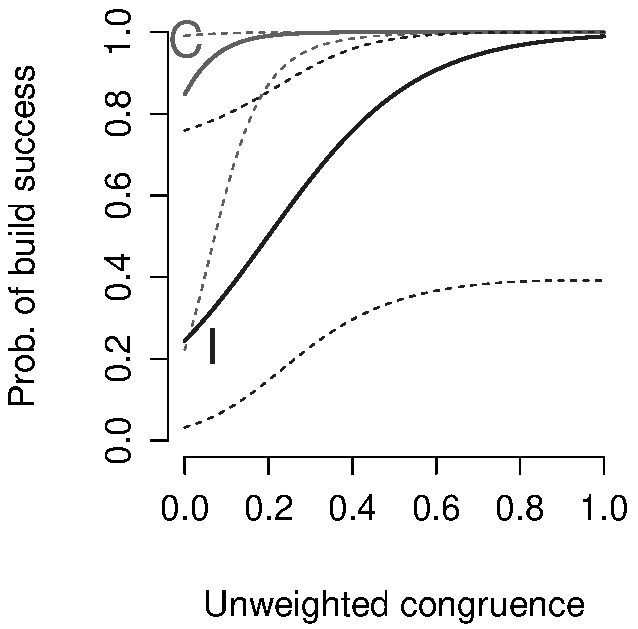
\includegraphics[scale=0.372]{prob_unweighted_age_typeci_q010}
    \label{subfig:prob_unweighted_age_typeci_q010}
  }
  \subfigure[ \small{2008-05-14} ]{
	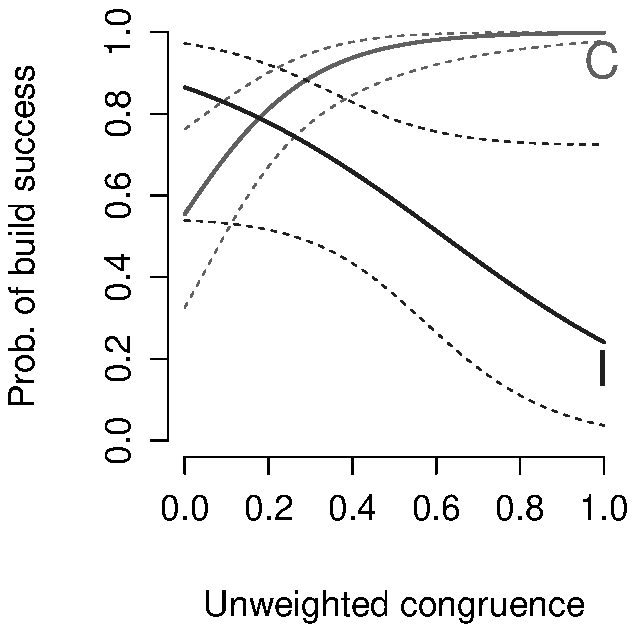
\includegraphics[scale=0.372]{prob_unweighted_age_typeci_q025}
     \label{subfig:prob_unweighted_age_typeci_q025}
  }
  \subfigure[ \small{2008-06-07} ]{
	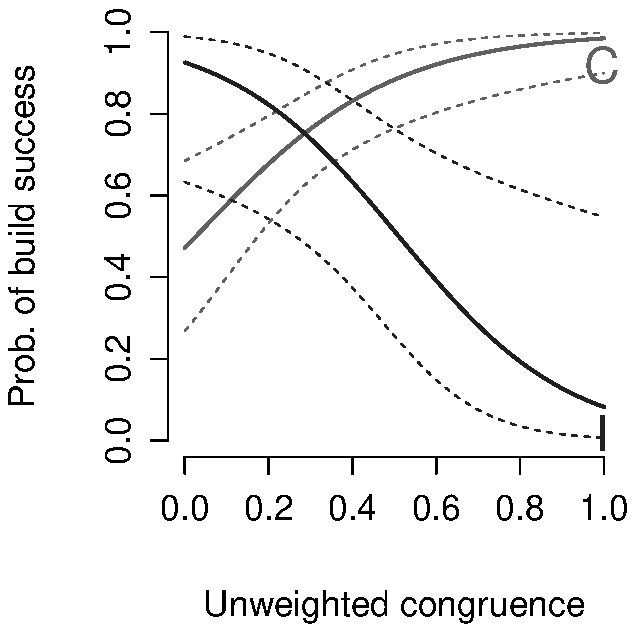
\includegraphics[scale=0.372]{prob_unweighted_age_typeci_q050}
     \label{subfig:prob_unweighted_age_typeci_q050}
  }
  \subfigure[ \small{2008-06-26} ]{
	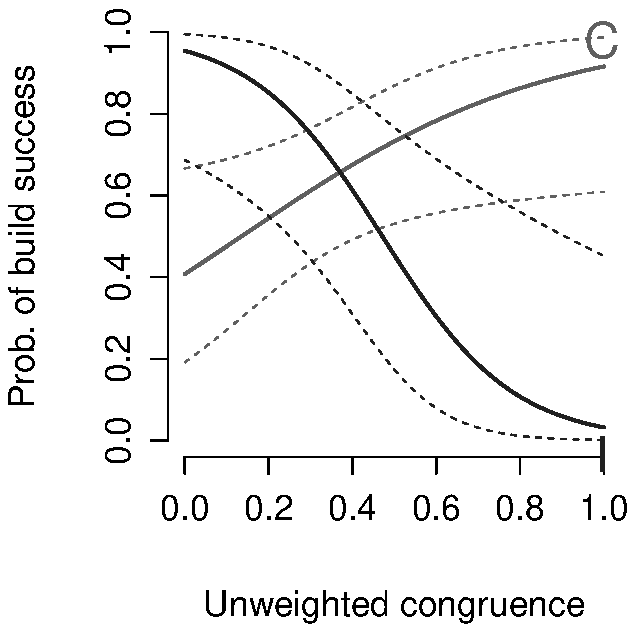
\includegraphics[scale=0.372]{prob_unweighted_age_typeci_q100}
     \label{subfig:prob_unweighted_age_typeci_q100}
  }
  
	\caption{Estimated probability of build success for \emph{unweighted congruence} and \emph{continuous builds C} or \emph{integration builds I}  over time, adjusted to authors $\approx$ -0.156 (17 authors), files $\approx$ -0.352 (131 files), work~items $\approx$ -0.399 (34 work items)}
	\label{fig:unweighted_congruence_typeci_age}
\end{figure*}

\begin{figure*}
\centering
  \subfigure[ \small{2008-01-25} ]{
    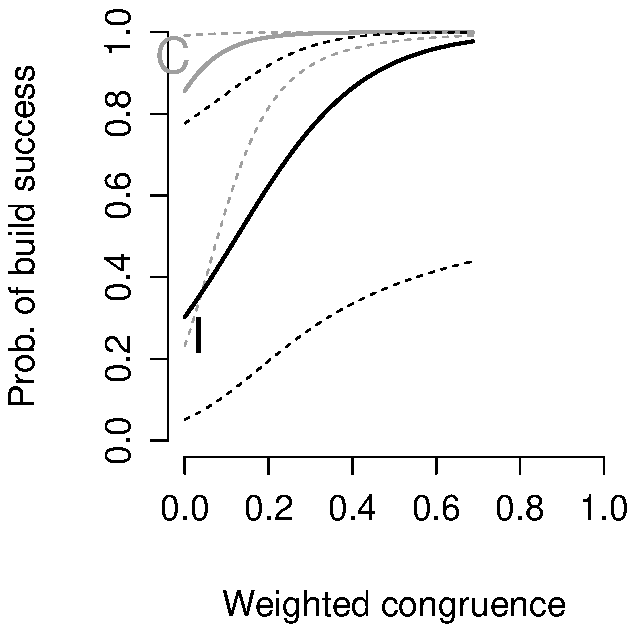
\includegraphics[scale=0.372]{prob_weighted_age_typeci_q010}
    \label{subfig:prob_weighted_age_typeci_q010}
  }
  \subfigure[ \small{2008-05-14} ]{
	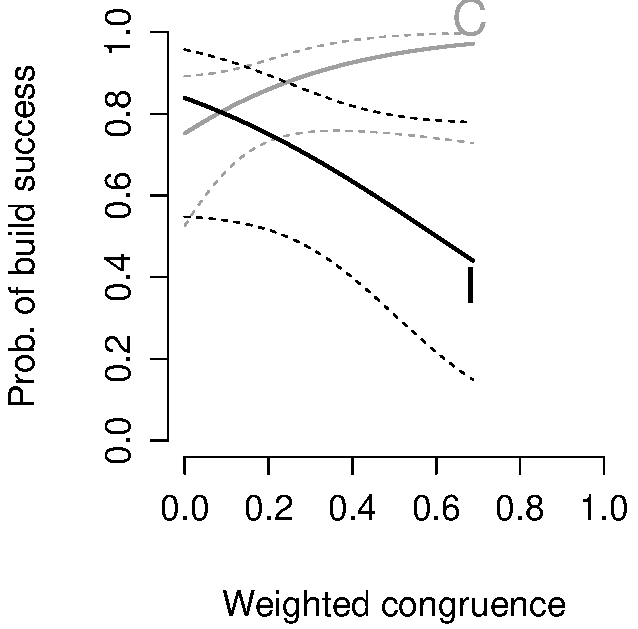
\includegraphics[scale=0.372]{prob_weighted_age_typeci_q025}
     \label{subfig:prob_weighted_age_typeci_q025}
  }
  \subfigure[ \small{2008-06-07} ]{
	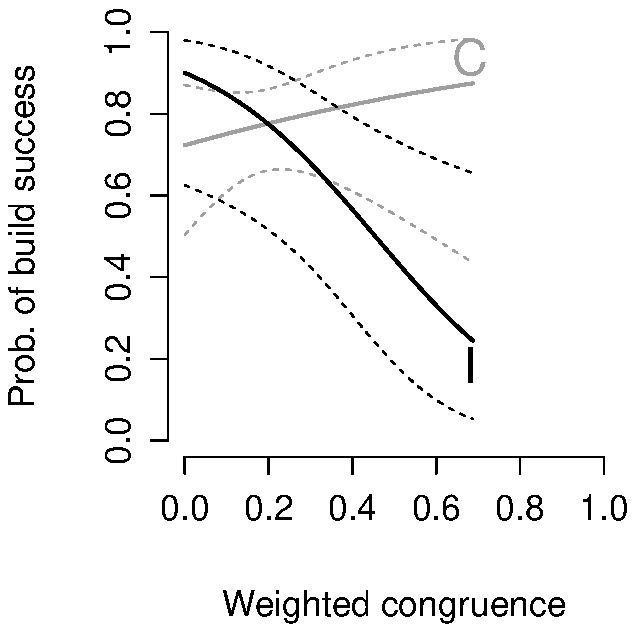
\includegraphics[scale=0.372]{prob_weighted_age_typeci_q050}
     \label{subfig:prob_weighted_age_typeci_q050}
  }
  \subfigure[ \small{2008-06-26} ]{
	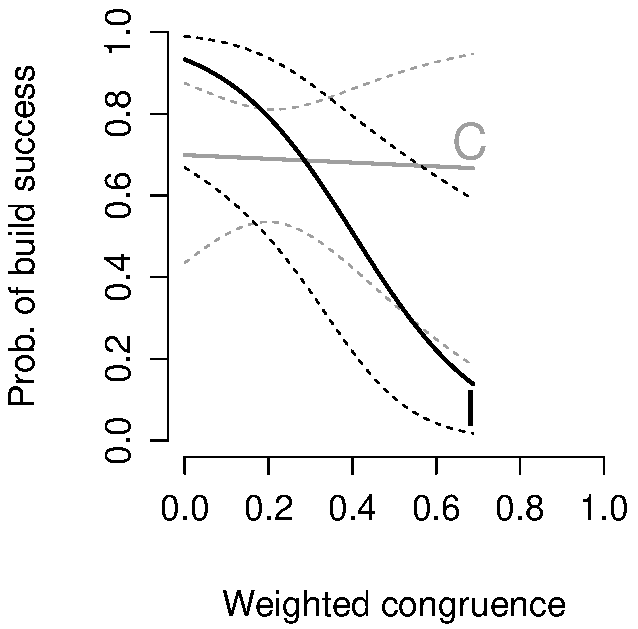
\includegraphics[scale=0.372]{prob_weighted_age_typeci_q100}
     \label{subfig:prob_weighted_age_typeci_q100}
  }
  
	\caption{Estimated probability of build success for \emph{weighted congruence} and \emph{continuous builds C} or \emph{integration builds I}  over time, adjusted to authors $\approx$ -0.156 (17 authors), files $\approx$ -0.352 (131 files), work~items $\approx$ -0.399 (34 work items)}
	\label{fig:weighted_congruence_typeci_age}
\end{figure*}

% The weighted and unweighted congruence models are very similar, and the effects on the variable for both models are the same. Consequently, we plot only weighted congruence probability plots to save space.


%We examine the relationship between congruence and build type on the build success probability using plots for each type of build across the life of the project. Our data contains 122 continuous builds, 55 nightly builds, and 14 integration builds. 

For continuous builds in weighted congruence (Figures \ref{fig:weighted_congruence_typeci_age}, in grey), an increase in congruence correlates to build success probability. The build date as the project ages appears to decrease the probability of build success for high-congruence builds more than low-congruence builds (Figure \ref{subfig:prob_weighted_age_typeci_q100}). Note that, in the unweighted congruence model (Table \ref{tab:logr}) the effect of unweighted congruence on continuous builds is significant, and that increasing congruence also increases the probability that a continuous build will succeed. However, the effect of weighted congruence in continuous builds is not as large as in unweighted congruence, nor is it considered statistically significant.

For integration builds (Figures \ref{fig:weighted_congruence_typeci_age}, in black), an increase in congruence decreases build success, with the exception of the 2008-01-25 build (Figure \ref{subfig:prob_weighted_age_typeci_q010}). In in our 2008-01-25 build, we see that low congruence leads to low build probability, but high congruence has high build probability. As the project ages, this trend reverses and congruence is clearly inversely related with build success probability (Figure \ref{subfig:prob_weighted_age_typeci_q100}).

The effect of congruence is totally opposite for continuous builds and integration builds in both unweighted and weighted congruence. Based on Figure \ref{subfig:prob_unweighted_age_typeci_q100}, increasing unweighted congruence significantly improves the continuous build success rate. However, increasing both types of congruence significantly decreases the integration build success rate.

% Nightly builds (Figures \ref{fig:weighted_congruence_typen_age}), are the most successful types of builds in RTC, and tend to succeed regardless of the congruence levels. % However the nightly builds also suffer from very wide confidence intervals, suggesting that a lack of data may have had an influence.

% The 95\% confidence intervals, indicated by the dashed lines and \ref{fig:weighted_congruence_summary} are extremely large. As congruence increases, the uncertainty of the effect on the probability of build success increases, suggesting that the relationship between congruence, type, and build success probability is vulnerable to being affected by other variables or random error. 


%For comparison, we illustrate in Figure \ref{} the effects of weighted congruence on build success using the same parameters, in which there is no significant interaction effect. We see a slight increase in build success when increasing weighted congruence in continuous builds (Figure \ref{subfig:prob_weighted_typeC}), but the confidence intervals also increase, decreasing the reliability. Both nightly builds (Figure \ref{subfig:prob_weighted_typeN}) and integration builds (Figure \ref{subfig:prob_weighted_typeI}) suggest no relationship between weighted congruence and build success probability.

%\begin{figure*}
%  \subfigure[ \small{2008-01-25} ]{
%    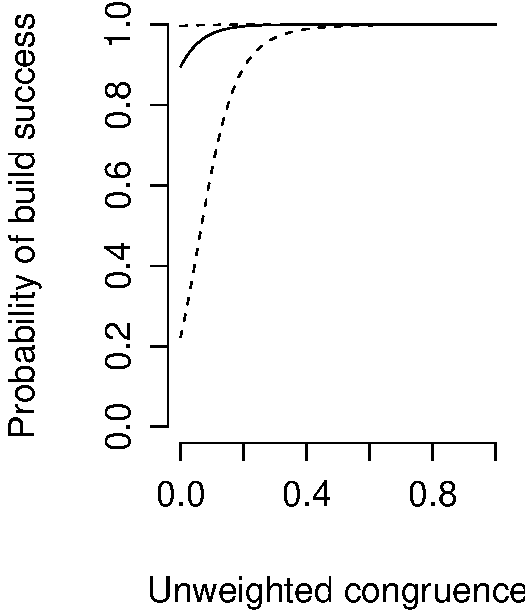
\includegraphics[scale=0.372]{prob_unweighted_age_typec_q010}
%    \label{subfig:prob_unweighted_age_typec_q010}
%  }
%  \subfigure[ \small{2008-05-14} ]{
%	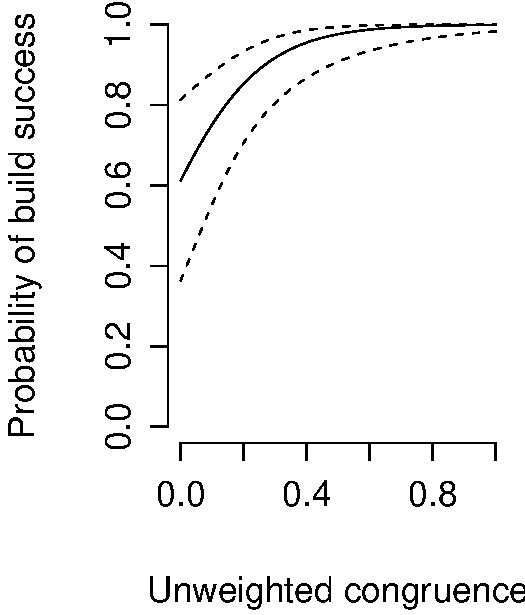
\includegraphics[scale=0.372]{prob_unweighted_age_typec_q025}
%     \label{subfig:prob_unweighted_age_typec_q025}
%  }
%  \subfigure[ \small{2008-06-07} ]{
%	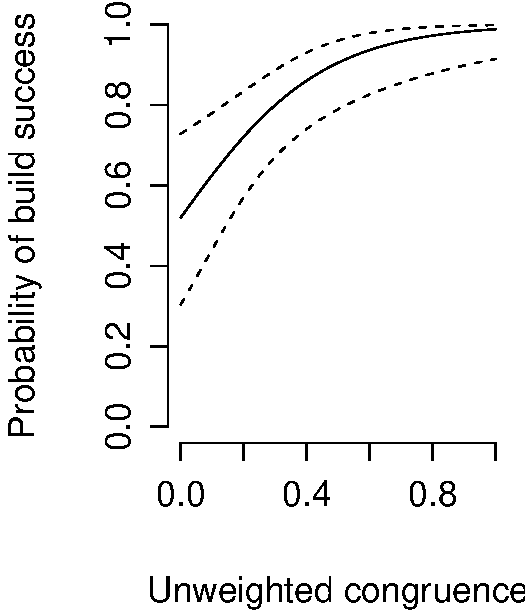
\includegraphics[scale=0.372]{prob_unweighted_age_typec_q050}
%     \label{subfig:prob_unweighted_age_typec_q050}
%  }
%  \subfigure[ \small{2008-06-18} ]{
%	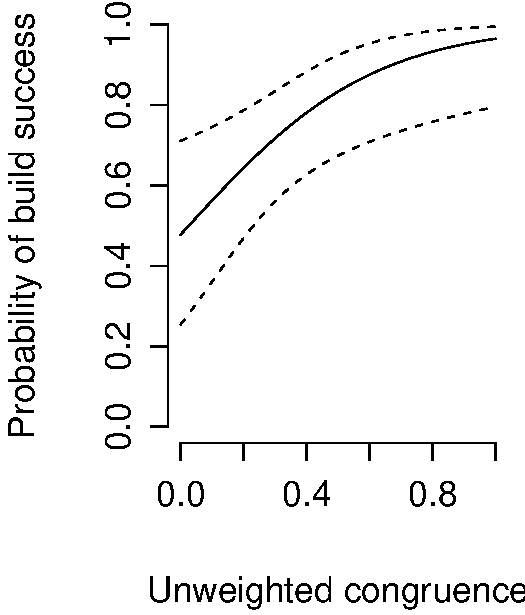
\includegraphics[scale=0.372]{prob_unweighted_age_typec_q075}
%     \label{subfig:prob_unweighted_age_typec_q075}
%  }
%  \subfigure[ \small{2008-06-26} ]{
%	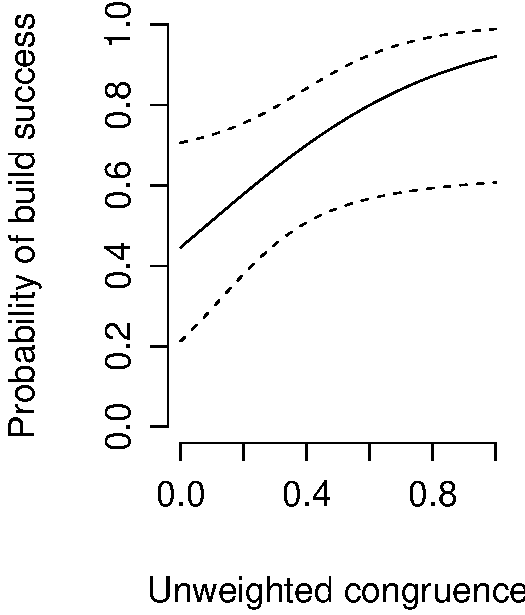
\includegraphics[scale=0.372]{prob_unweighted_age_typec_q100}
%     \label{subfig:prob_unweighted_age_typec_q100}
%  }
%  
%	\caption{Estimated probability of build success for \emph{unweighted congruence and date}, adjusted to authors $\approx$ -0.156 (17), files $\approx$ -0.352 (131), workitems $\approx$ -0.399 (34), type = cont.}
%	\label{fig:unweighted_congruence_age}
%\end{figure*}

%\begin{figure*}
%  \subfigure[ \small{2008-01-25} ]{
%    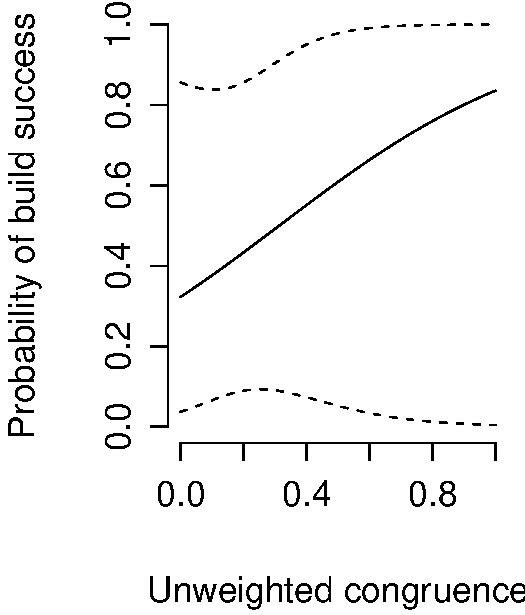
\includegraphics[scale=0.372]{prob_unweighted_age_typei_q010}
%    \label{subfig:prob_unweighted_age_typei_q010}
%  }
%  \subfigure[ \small{2008-05-14} ]{
%	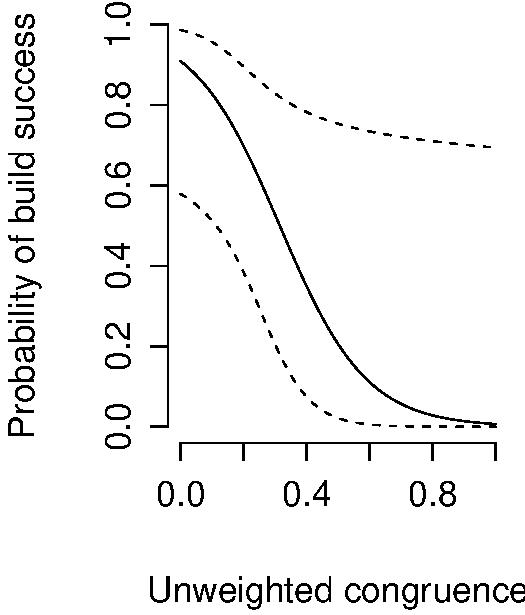
\includegraphics[scale=0.372]{prob_unweighted_age_typei_q025}
%     \label{subfig:prob_unweighted_age_typei_q025}
%  }
%  \subfigure[ \small{2008-06-07} ]{
%	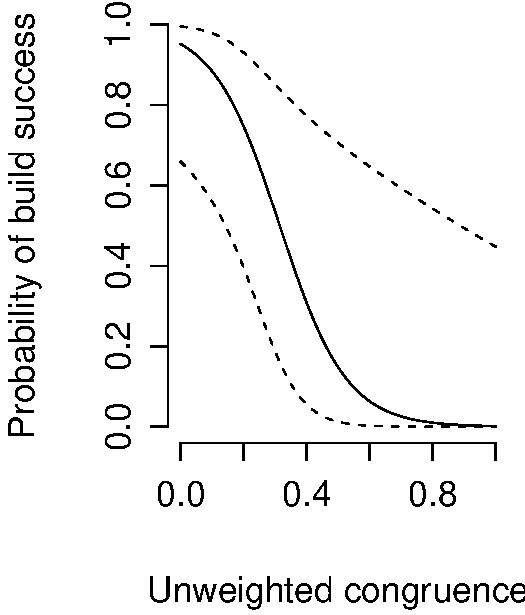
\includegraphics[scale=0.372]{prob_unweighted_age_typei_q050}
%     \label{subfig:prob_unweighted_age_typei_q050}
%  }
%  \subfigure[ \small{2008-06-18} ]{
%	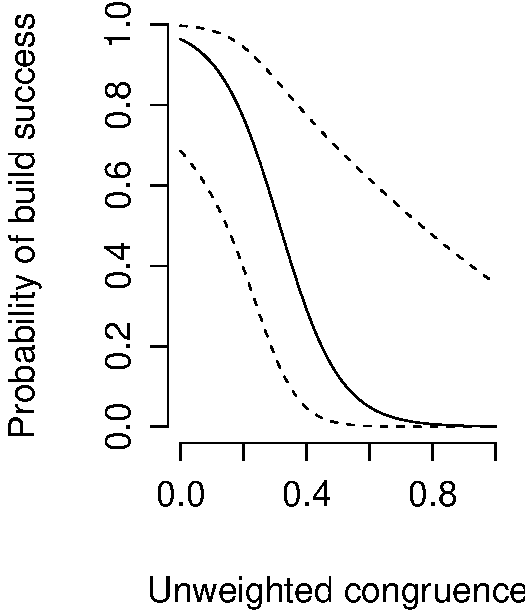
\includegraphics[scale=0.372]{prob_unweighted_age_typei_q075}
%     \label{subfig:prob_unweighted_age_typei_q075}
%  }
%  \subfigure[ \small{2008-06-26} ]{
%	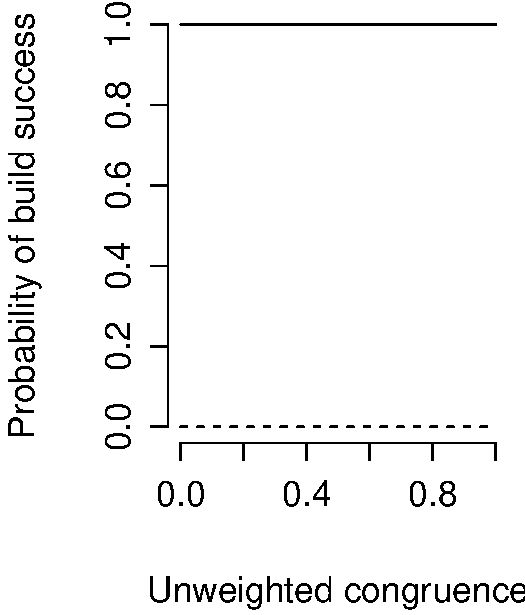
\includegraphics[scale=0.372]{prob_unweighted_age_typei_q100}
%     \label{subfig:prob_unweighted_age_typei_q100}
%  }
%  
%	\caption{Estimated probability of build success for \emph{unweighted congruence and date}. adjusted to authors $\approx$ -0.156 (17), files $\approx$ -0.352 (131), workitems $\approx$ -0.399 (34), type = int.}
%	\label{fig:unweighted_congruence_age}
%\end{figure*}

%\begin{figure*}
%  \subfigure[ \small{2008-01-25} ]{
%    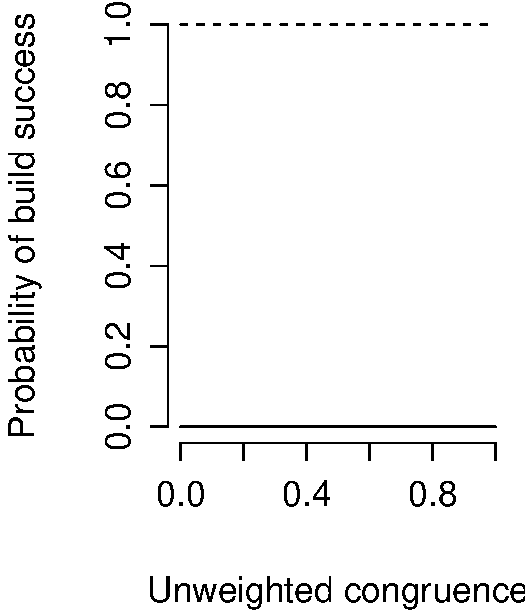
\includegraphics[scale=0.372]{prob_unweighted_age_typen_q010}
%    \label{subfig:prob_unweighted_age_typen_q010}
%  }
%  \subfigure[ \small{2008-05-14} ]{
%	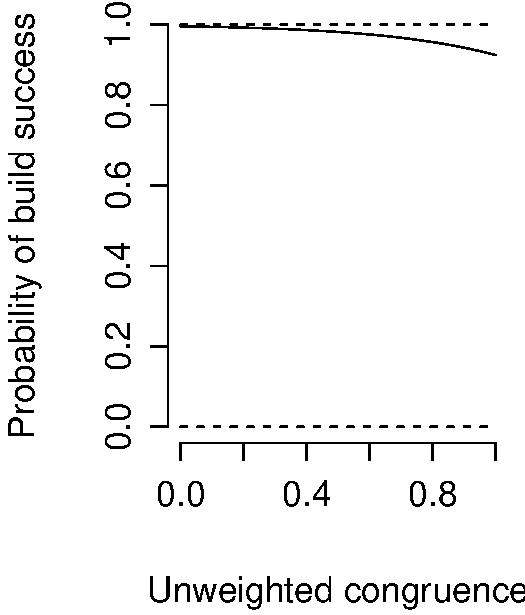
\includegraphics[scale=0.372]{prob_unweighted_age_typen_q025}
%     \label{subfig:prob_unweighted_age_typen_q025}
%  }
%  \subfigure[ \small{2008-06-07} ]{
%	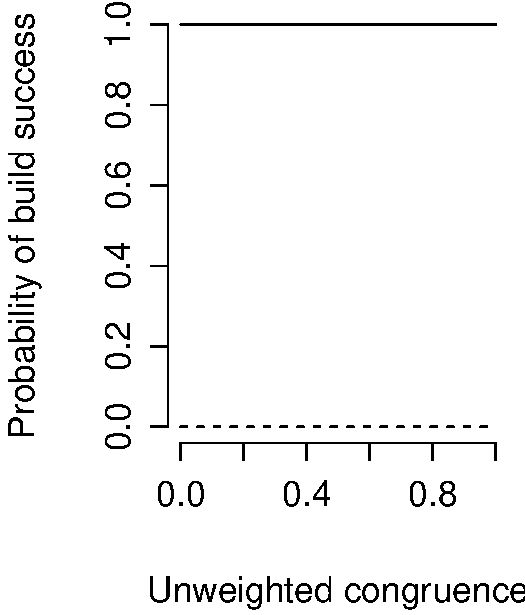
\includegraphics[scale=0.372]{prob_unweighted_age_typen_q050}
%     \label{subfig:prob_unweighted_age_typen_q050}
%  }
%  \subfigure[ \small{2008-06-18} ]{
%	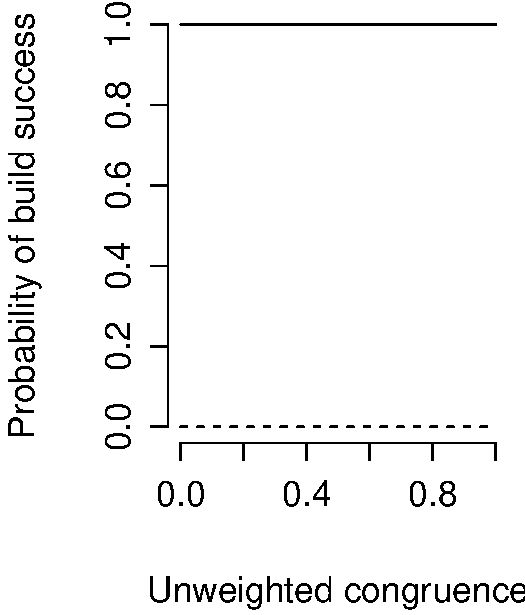
\includegraphics[scale=0.372]{prob_unweighted_age_typen_q075}
%     \label{subfig:prob_unweighted_age_typen_q075}
%  }
%  \subfigure[ \small{2008-06-26} ]{
%	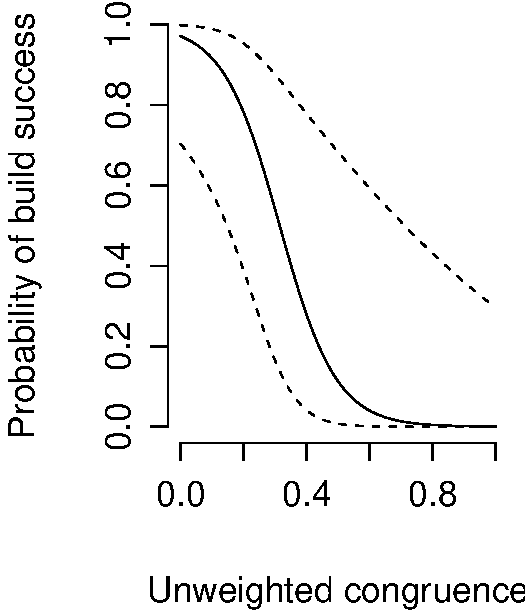
\includegraphics[scale=0.372]{prob_unweighted_age_typen_q100}
%     \label{subfig:prob_unweighted_age_typen_q100}
%  }
%  
%	\caption{Estimated probability of build success for \emph{unweighted congruence and date}. adjusted to authors $\approx$ -0.156 (17), files $\approx$ -0.352 (131), workitems $\approx$ -0.399 (34), type = night.}
%	\label{fig:unweighted_congruence_age}
%\end{figure*}




%\begin{figure*}
%  \subfigure[ \small{2008-01-25} ]{
%    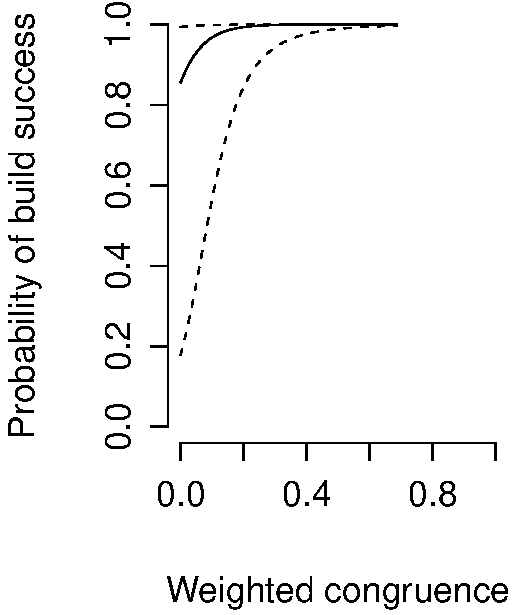
\includegraphics[scale=0.372]{prob_weighted_age_typec_q010}
%    \label{subfig:prob_weighted_age_typec_q010}
%  }
%  \subfigure[ \small{2008-05-14} ]{
%	\includegraphics[scale=0.372]{prob_weighted_age_typec_q025}
%     \label{subfig:prob_weighted_age_typec_q025}
%  }
%  \subfigure[ \small{2008-06-07} ]{
%	\includegraphics[scale=0.372]{prob_weighted_age_typec_q050}
%     \label{subfig:prob_weighted_age_typec_q050}
%  }
%  \subfigure[ \small{2008-06-18} ]{
%	\includegraphics[scale=0.372]{prob_weighted_age_typec_q075}
%     \label{subfig:prob_weighted_age_typec_q075}
%  }
%  \subfigure[ \small{2008-06-26} ]{
%	\includegraphics[scale=0.372]{prob_weighted_age_typec_q100}
%     \label{subfig:prob_weighted_age_typec_q100}
%  }
%  
%	\caption{Estimated probability of build success for \emph{weighted congruence} and \emph{build date} for \emph{continuous builds}, adjusted to authors $\approx$ -0.156 (17 authors), files $\approx$ -0.352 (131 files), workitems $\approx$ -0.399 (34 work items)}
%	\label{fig:weighted_congruence_typec_age}
%\end{figure*}

%\begin{figure*}
%  \subfigure[ \small{2008-01-25} ]{
%    \includegraphics[scale=0.372]{prob_weighted_age_typei_q010}
%    \label{subfig:prob_weighted_age_typei_q010}
%  }
%  \subfigure[ \small{2008-05-14} ]{
%	\includegraphics[scale=0.372]{prob_weighted_age_typei_q025}
%     \label{subfig:prob_weighted_age_typei_q025}
%  }
%  \subfigure[ \small{2008-06-07} ]{
%	\includegraphics[scale=0.372]{prob_weighted_age_typei_q050}
%     \label{subfig:prob_weighted_age_typei_q050}
%  }
%  \subfigure[ \small{2008-06-18} ]{
%	\includegraphics[scale=0.372]{prob_weighted_age_typei_q075}
%     \label{subfig:prob_weighted_age_typei_q075}
%  }
%  \subfigure[ \small{2008-06-26} ]{
%	\includegraphics[scale=0.372]{prob_weighted_age_typei_q100}
%     \label{subfig:prob_weighted_age_typei_q100}
%  }
%  
%	\caption{Estimated probability of build success for \emph{weighted congruence} and \emph{build date} for \emph{integration builds}, adjusted to authors $\approx$ -0.156 (17), files $\approx$ -0.352 (131), workitems $\approx$ -0.399 (34)}
%	\label{fig:weighted_congruence_typei_age}
%\end{figure*}

%\begin{figure*}
%  \subfigure[ \small{2008-01-25} ]{
%    \includegraphics[scale=0.372]{prob_weighted_age_typen_q010}
%    \label{subfig:prob_weighted_age_typen_q010}
%  }
%  \subfigure[ \small{2008-05-14} ]{
%	\includegraphics[scale=0.372]{prob_weighted_age_typen_q025}
%     \label{subfig:prob_weighted_age_typen_q025}
%  }
%  \subfigure[ \small{2008-06-07} ]{
%	\includegraphics[scale=0.372]{prob_weighted_age_typen_q050}
%     \label{subfig:prob_weighted_age_typen_q050}
%  }
%  \subfigure[ \small{2008-06-18} ]{
%	\includegraphics[scale=0.372]{prob_weighted_age_typen_q075}
%     \label{subfig:prob_weighted_age_typen_q075}
%  }
%  \subfigure[ \small{2008-06-26} ]{
%	\includegraphics[scale=0.372]{prob_weighted_age_typen_q100}
%     \label{subfig:prob_weighted_age_typen_q100}
%  }
%  
%	\caption{Estimated probability of build success for \emph{weighted congruence} and \emph{build date} for \emph{nightly builds}, adjusted to authors $\approx$ -0.156 (17), files $\approx$ -0.352 (131), workitems $\approx$ -0.399 (34)}
%	\label{fig:weighted_congruence_typen_age}
%\end{figure*}


%\subsubsection{Effect of Number of Work Items}

%Another influence on socio-technical congruence is the number of work items that
%a build is involved in. A work item is of interest in RTC because it represents
%a unit of work. We would expect to see an inverse correlation between the number
%of work items and congruence on the rationale that the more work items that are involved
%in the build, the harder it is for people to coordinate.

%To count the number of work items in a build, we identify the change sets in each build. Each change set is attached to a work item. Our results indicate that the number of work items range from 4 up to 182, with a mean value of 42.54 work items per build. The distribution is highly skewed to the left.

%From our previous models (Tables \ref{tab:logr_unweighted} and \ref{tab:logr_weighted}), which feature the number of work items per build as a variable, there is no significant effect of the number of work items on the build result.

%A correlation test using the Spearman $\rho$ method on the number of work items per build versus unweighted congruence indicated that there was no correlation between the number of work items, and congruence (S = 2.04e+12, p-value~=~0.7869, $\rho = -0.00178$).

%The same correlation test on the number of work items per build versus weighted
%congruence indicated also that there is correlation
%between the number of work items and unweighted congruence (S = 1.88e+12, p-value $<$ 2.2e-16, $\rho = 0.0794$), but because the $\rho$ value is so low, these results are not reliable.

%\begin{figure}
%	\centering
%	\includegraphics[scale=0.5]{figures/boxplot_numworkitems}
%	\caption{Boxplot of Average Number of Work Items Referred to in OK builds and error builds}
%	\label{fig:numworkitems}
%\end{figure}

%We also investigate the relationship between the number of work items and build result. There is a statistically significant difference between the mean number of work items involved in an error build compared to an OK build (W = 61046557, p-value $<$ 2.2e-16) (Figure \ref{fig:numworkitems}).



\subsection{Effect of Gap Size on Build Result}
\label{sec:gapsizeresult}

To answer Research Question 2, we fit a logistic regression model to determine the effect of the mean gap size on the build success probability. The mean gap size appears in Table \ref{tab:summary} and Figure \ref{fig:gapsizes}.
% For error builds, the values range from -0.0405 to 1.0, with a mean of 0.147. For OK builds, the values range from -0.0834 to 1.0, with a mean of 0.391.

%For interest, we adjusted the gap size and limited it to the ranges 0 and 1. A Mann-Whitney test between the gap size and the adjusted gap size illustrates that the difference in means is not significant (W = 18048.5, p = 0.859) and a logistic regression analysis using adjusted gap size instead of gap size with negative values revealed no differences.

We build logistic regression models based on the model in Table \ref{tab:logr} using the gap size measurement. In the interest of saving space, we report only the odds ratio. We retain every significant interaction from our previous weighted congruence logistic regression in Table \ref{tab:logr}.
We compare two different models: Model G1 contains the gap size with weighted congruence as a variable, and Model G2 contains the gap size without weighted congruence.  We do not use unweighted congruence as it is not possible to calculate gap size with unweighted congruence.

The effect of gap size on build result is significant in both models (Table \ref{tab:oddsratio_gapsize}). This indicates that increasing the gap size significantly increases the odds that an OK build will occur, which is the opposite of what we hypothesized (Figure \ref{fig:prob_gapsize_a}). This means that if the gap size is large, the build success probability increases.

%\begin{figure}
%	\centering
%  \subfigure[Gap Size (H1)]{
%	\includegraphics[scale=0.55]{prob_gapsize_5a}
%	\label{subfig:prob_gapsize_a}
%  }
%  \subfigure[Gap size (H2)]{
%	\includegraphics[scale=0.55]{prob_gapsize_6b}
%     \label{subfig:prob_gapsize_6a}
%  }
%	\caption{Effect of Gap Size on build success (authors = 17, files = 131, change sets = 34, type = continuous, and weighted cong = 0.1446)}
%	\label{fig:prob_gapsize_a}
%\end{figure}

% latex table generated in R 2.11.0 by xtable 1.5-6 package
% Mon Sep 13 10:39:05 2010
\begin{table}[h]
\begin{center}
\begin{tabular}{l|rr}
  \hline
 & Model G1 & Model G2 \\ 
  \hline
Intercept & 0.95 & 1.32 \\ 
  Authors & 0.43 & 0.60 \\ 
  Files & 0.63 & 0.63 \\ 
  Work~items & 0.75 & 0.85 \\ 
  Build type=I & 4.22 & 1.31 \\ 
  Weighted cong & 8.41 & - \\ 
  Gapsize & 7.71 & 8.71 \\ 
  Build date & 1.81 & 0.59 \\ 
  Authors * Build date & 0.40 & 0.74 \\ 
  Work~items * Build date & 2.75 & 1.83 \\ 
  Build type=I * Build date & 3.54 & 2.52 \\ 
  Build type=I * Weighted cong & 0.01 & - \\ 
  Weighted cong * Build date & 0.00 & - \\ 
   \hline
\end{tabular}
\caption{Odds Ratio for Gapsize Models}
\label{tab:oddsratio_gapsize}
\end{center}
\end{table}


\begin{figure}[t]
\begin{minipage}[b]{0.4\linewidth}
	\centering	
	\includegraphics[scale=0.372]{boxplot_meangapsize}
	\caption{Mean Gap Size per Build}
	\label{fig:gapsizes}
\end{minipage}
%\end{figure}
\hspace{0.5cm}
%\begin{figure}
\begin{minipage}[b]{0.4\linewidth}
	\centering
	\includegraphics[scale=0.372]{prob_gapsize_g1}
	\caption{Effect of gap size on build success probability, model G1. }
	\label{fig:prob_gapsize_a}
\end{minipage}
\end{figure}

% Adjusted to authors $\approx$ -0.156 (17), workitems $\approx$ {-0.399} (34), type=cont, weightedCong $\approx$ 0.1446, date $\approx$ 2008-06-07)



\subsection{Social and Technical Factors in RTC Affecting Build Success and Congruence}
\label{sec:otherfactors}

% In light of the results of Research Questions 1 and 2, we perform additional analysis on other variables that may affect the probability of build success.
In light of our results, we examine not only the number of work~items~$\times$~date significant interaction found in Section \ref{sec:congruence_effect_build_result}, but different social and technical factors that may affect congruence
and build success probability to find explanations for the interactions between socio-technical congruence and build success probability in RTC.
Specifically, we examine the effect of build date on work items, coordination around fully-congruent builds and
incongruent builds, and the effects of commenting behaviour on builds.

% After adding the "date" variable, authors * files is no longer significant.
%
%\subsubsection{Effect of Authors and Files on build success probability}

%
%The unweighted~congruence~$\times$~build~type interaction is not the only significant variable affecting build result rate. There is a significant interaction between authors and files in both unweighted and weighted congruence (Table \ref{tab:logr_unweighted}). 

%\TODO[FIX THIS] The scatterplot visualization of this data (Figure \ref{fig:scatter_authors_files}) reveals that though most of the builds involve under 500 files, the number of authors across these builds varies from 2 authors to 44 authors.

%To explore this interaction, we plot the effect of the number of files on the probability of build success for different numbers of authors while holding the other variables at fixed values. We show the unweighted congruence plots in Figure \ref{fig:files_authors_unweighted}. Since the effect of authors $\times$ files on build success probability is similar in the weighted and unweighted congruence cases, we do not show the weighted congruence plots to save space. The baseline for comparison is 35 authors, which we chose because it is the level at which the effect of files on build success probability is not extremely pronounced (Figure \ref{subfig:prob_unweighted_35authors}). We do not include the graphs for weighted congruence for space reasons, but the plots for weighted congruence are almost identical to their unweighted congruence counterparts.

%\TODO[FIX THIS TOO] When the number of files is low---700 and below---having a small number of authors involved in the build increases the chance that the build outcome will be successful (Figure \ref{subfig:prob_unweighted_02authors}). Increasing the number of files drastically decreases the probability of build success (Figure \ref{subfig:prob_unweighted_44authors}). However, as more authors contribute to the build, build success decreases when the number of files is low, but build success increases when the number of files are high.


\subsubsection{Other Effects on Build Success}
\label{sec:effectauthors}

\indent\indent
\textbf{Authors} For both weighted and unweighted congruence, as the number of authors involved in a build increases, the probability that the build succeeds decreases. The build probability is significantly lowered after more than 15 authors are involved in the build (Figure \ref{subfig:prob_weighted_authors_age_q100}). When over 30 authors are involved in the build, the estimated build success probability falls under 10\%.

\begin{figure}[b]
\centering
\subfigure[ \small{Authors} ] {
\includegraphics[scale=0.372]{prob_weighted_authors_age_q100}
\label{subfig:prob_weighted_authors_age_q100}
}
\subfigure[ \small{Files} ] {
\includegraphics[scale=0.372]{prob_weighted_files_age_q100}
\label{subfig:prob_weighted_files_age_q100}
}

\caption{Estimated probability of build success for \emph{authors} and \emph{files}, weighted congruence. Adjusted to work~items $\approx$ -0.399 (34), authors $\approx$ -0.156 (17), files $\approx$ -0.352 (131), w. congruence $\approx$ 0.1446, type = cont, date=2008-06-26}
  \label{fig:weighted_congruence_authors_age}
\end{figure}



\textbf{Files} For both weighted and unweighted congruence, as the number of files involved in a build increases, the probability that the build will succeed decreases (Figure \ref{subfig:prob_weighted_files_age_q100}).

\textbf{Build Date and Work items} The work~items~$\times$~date interaction is significant in both weighted and unweighted congruence. Early in the project, as the number of work items increases, the probability of build success decreases (Figure \ref{subfig:prob_weighted_workitems_age_q010}). As the project ages, this trend reverses and as the number of work items increases, the probability of build success increases as well (Figure \ref{subfig:prob_weighted_workitems_age_q100}). According to the coefficients in Table \ref{tab:logr}, this effect on build success probability is not as strong as the authors main effect or the files main effect.

\begin{figure}[b]
\centering
  \subfigure[ \small{2008-01-25} ]{
    \includegraphics[scale=0.372]{prob_weighted_workitems_x_age_q010}
    \label{subfig:prob_weighted_workitems_age_q010}
  }
%  \subfigure[ \small{2008-05-14} ]{
%	\includegraphics[scale=0.372]{prob_weighted_workitems_x_age_q025}
%     \label{subfig:prob_weighted_workitems_age_q025}
%  }
%  \subfigure[ \small{2008-06-07} ]{
%	\includegraphics[scale=0.372]{prob_weighted_workitems_x_age_q050}
%     \label{subfig:prob_weighted_workitems_age_q050}
%  }
  %\subfigure[ \small{2008-06-18} ]{
	%\includegraphics[scale=0.372]{prob_weighted_workitems_x_age_q075}
     %\label{subfig:prob_weighted_workitems_age_q075}
  %}
  \subfigure[ \small{2008-06-26} ]{
	\includegraphics[scale=0.372]{prob_weighted_workitems_x_age_q100}
     \label{subfig:prob_weighted_workitems_age_q100}
  }
  \caption{Estimated probability of build success for \emph{work items} and \emph{date}, weighted congruence. Adjusted to authors $\approx$ -0.156 (17), files $\approx$ -0.352 (131), w. congruence $\approx$ 0.1446, type = cont}
  \label{fig:weighted_congruence_workitems_age}
\end{figure}


%\begin{figure*}
%\centering
%  \subfigure[ \small{2008-01-25} ]{
%    \includegraphics[scale=0.372]{prob_weighted_authors_age_q010}
%    \label{subfig:prob_weighted_workitems_age_q010}
%  }
%  \subfigure[ \small{2008-05-14} ]{
%	\includegraphics[scale=0.372]{prob_weighted_authors_age_q025}
%     \label{subfig:prob_weighted_workitems_age_q025}
%  }
%  \subfigure[ \small{2008-06-07} ]{
%	\includegraphics[scale=0.372]{prob_weighted_authors_age_q050}
%     \label{subfig:prob_weighted_workitems_age_q050}
%  }
%  \subfigure[ \small{2008-06-26} ]{
%	\includegraphics[scale=0.372]{prob_weighted_authors_age_q100}
%     \label{subfig:prob_weighted_workitems_age_q100}
%  }
%  \caption{Estimated probability of build success for \emph{authors} and \emph{date}, weighted congruence. Adjusted to workitems $\approx$ -0.399 (34), files $\approx$ -0.352 (131), weighted congruence $\approx$ 0.1446, type = cont}
%  \label{fig:weighted_congruence_authors_age}
%\end{figure*}

\subsubsection{Commenting Behaviour by Change Set Authors}
\label{sec:commenting}

As congruence expects those who contribute technical work to a project to also communicate changes, we decided to examine commenting behaviour of change set contributors.
We examine whether a work item related to a change set has a corresponding comment posted by the change set's author. We also identify if the work item/change set pair is involved in an OK build or an Error build. Note that a work item/change set pair can occur in multiple builds. We consider only comments posted before the build was started. These results are shown in Table \ref{tab:changesets_authors}.
The build result rates does not appear to be affected by whether the change set contributor commented: 43\% of the builds resulted in error when the contributor commented, and 41\% of builds resulted in error when the contributor did not comment. A $\chi^2$ test on this table does not show a significant difference between the factors at the 0.05 threshold ($\chi^2 = 3.217$, df = 1, {p=0.073}).
Overall, in 76\% of the change set/work item pairs, the change set contributor also posted a comment in the associated work item.
\begin{table}[t]
\centering
\begin{tabular}{lrrr}
Result & \parbox{0.715in}{\raggedright Change sets w/o comment by contributor\vspace{1pt}} & \parbox{0.715in}{\raggedright Change sets w/ comment by contributor\vspace{1pt}} & Total \\\hline 
OK		& 1278 (14\%) 	& 3956 (43\%) 	& 5234 (57\%) 	\\
ERR		& 908 (10\%) 	& 3076 (33\%)	& 3984 (43\%)	\\\hline
Total 	& 2186 (24\%) 	& 7032 (76\%) 	& 9218 (100\%)	\\
\end{tabular}
\caption{Number of change sets in which a contributor commented in the corresponding work item}
\label{tab:changesets_authors}
\end{table}

% We then examined the amount of communication that occurs over coordination needs between pairs of individuals. Over 95\% of the coordination needs in the project are not satisfied by a corresponding communication edge between the developers.

\subsubsection{Examining Extreme Congruence Values}
\label{sec:extremecongruence}

We are interested in the differences between high-congruence builds and low-congruence builds.
We further this investigation by looking at builds that have extreme values of congruence: zero, where absolutely no coordination needs are satisfied with communication, and one, where every coordination need is satisfied with communication.
%A congruence index of 0 means that absolutely no actual coordination occurs where a coordination need exists.
%A congruence index of 1 means that actual coordination occurs for every coordination need that exists.
We chose to investigate the extreme cases to see if there were differences in the way people coordinated in fully-congruent builds, and in incongruent builds.
Table \ref{tab:congruence_extremes} shows the number of OK and error builds that occurred when congruence was equal to one, and equal to zero. The weighted builds with full congruence are a subset of the unweighted builds with full congruence.

%In our data, 32 builds have both a weighted and unweighted congruence index of 0. Among these builds, 2 of them are error builds and 30 are OK builds. It appears that, even in a situation with with 0 congruence, the majority of these builds appeared to have built successfully.

% We then examine the builds that have a congruence of 1, which suggests ``perfect congruence''. There are 26 builds that have an unweighted congruence index of 1; of these builds, 2 builds are error builds and 26 are OK builds. For weighted congruence, there are 7 builds that have a weighted congruence of 1; 1 build is an error build and 6 are OK builds. The weighted congruence builds are subsets of the unweighted congruence builds.

\begin{table}[t]
\centering
\begin{tabular}{ll|rr}
& & \multicolumn{2}{c}{Congruence} \\\hline
&  & 1 & 0 \\\hline 
\multirow{2}{*}{Unweighted} & OK & 26 & 30 \\
                            & ERR & 2 & 2 \\\hline
\multirow{2}{*}{Weighted} & OK & 6 & 30 \\
                         & ERR & 1 & 2 \\
\end{tabular}
\caption{Number of Builds with Congruence Values 0 and 1}
\label{tab:congruence_extremes}
\end{table}



% \texttt{28  44  55  66  71  76  86  104 123 144 147 164 171 172 176 194 210 222 239 246 248 250 256 268 289 292 313 321 336 337 341 347 354}, 33 builds.



%Weighted congruence \texttt{143 177 190 213 226 283 327}, 7 builds.
%Nonweighted congruence \texttt{5   32  42  43  57  63  64  77  80  93  111 113 143 163 170 177 179 190 213 226 266 269 283 297 324 327 355 356}, 28 builds.
% weighted = 0 \texttt{143 177 190 213 226 283 327},
% weighted error: (177)
% unweighted error: build 177 but also build 93. 


To determine if the presence of commenting affected the builds, we examined the number of comments on work item--change set pairs in builds with extreme unweighted congruence values. Our results are shown in Table \ref{tab:changeset_commenters}. Build success probabilities improve with respect to builds that have no comments, though work items with no comments are in the minority.

Of note is the high number of comments on work items that have zero congruence. This indicates that individuals who have no technical relationship to the work item are commenting on the work item.

\begin{table}[t]
\centering
\begin{tabular}{ll|rr|rr}
& & \multicolumn{2}{c|}{Num. of Pairs} & \multicolumn{2}{c}{Success rate} \\
Congruence &                                & 1     & 0   & 1 & 0 \\\hline 
\multirow{2}{*}{No comments} 	& OK 	  & 42   & 143  &  \multirow{2}{*}{49\%} & \multirow{2}{*}{69\%}  \\
                            	& Error   & 43    & 64   &  & \\\hline
\multirow{2}{*}{Comments} 	& OK 	  & 610  & 445  & \multirow{2}{*}{68\%} & \multirow{2}{*}{69\%}  \\
                         	& Error   & 290   & 199  &  & \\\hline
\multirow{2}{*}{Total} 		& OK		  & 652 & 588 &     \multirow{2}{*}{66\%} & \multirow{2}{*}{69\%}   \\
                       		& Error   & 333  & 263 & &\\
\end{tabular}
\caption{Number of work items-change set pairs with comments and build success probabilities for congruence 0 and 1}
\label{tab:changeset_commenters}
\end{table}

We manually inspected the work items with extreme amounts of congruence, reading the comments for any differences in the content discussed. Unfortunately, there were no obvious qualities between comments made in a build with a congruence of zero, and comments made in a build with a congruence of one. In both builds, individuals discussed technical implementation details, provided updates to colleagues, or requested assistance from colleagues. We are unable to discover root causes of failure without a deeper examination of the technical changes and more knowledge of the RTC context.
% Another observation made from reading the comments is that these work items for the cases where congruence is 0 or 1 do not appear to have strong dependencies on other work items.


\section{Discussion}
\label{sec:discussion}

The concepts illustrated in Conway's Law, as well as previous empirical work on socio-technical congruence lead us to expect that team members must coordinate according to coordination needs suggested by technical dependencies in order to build software effectively.
In this case study, we applied socio-technical congruence to study coordination and its relationship to build success probability in RTC. We applied a modified weighted congruence measurement to study also how the size of a coordination gap affects build success probability, and investigated what social and technical factors in RTC affect congruence and builds.

Overall, we found that the average congruence across builds was very low---only 20--30\% of the coordination needs in the project were fulfilled with actual coordination. Even in the cases where there is zero congruence, the build result was an OK build in over 90\% of the observed cases.

Our first research question asked:
\textbf{Does socio-technical congruence have an effect on build success probability in RTC?}
We found that there was an interaction effect involving congruence and build type on build success probabilities (Section \ref{sec:congruenceinteractions}). For continuous builds, increasing congruence improves the chance of build success in continuous builds and can actually decrease build success probability in integration builds (Figures \ref{fig:weighted_congruence_typeci_age}). High unweighted congruence significantly improves continuous build success probability, and both unweighted and weighted congruence significantly reduce integration build success probability.

Our second research question asked:
\textbf{Does gap size have an effect on build success probability
in RTC?}
The gap size is a representation of whether enough coordination
occurred to fulfill multiple coordination needs. If two developers have multiple dependencies on each other, one would expect them to
coordinate more often as well.
We hypothesized that a small mean gap size would increase the probability of successful builds and that a large mean gap size would decrease the probability of a successful build. Instead, we found that as the mean gap size increases, the build success probability also increases (Figure \ref{fig:prob_gapsize_a}).

Below we discuss the reasons for these observed results based on our knowledge of RTC.

\subsection{Strong Awareness Helps Coordination}

The overall congruence for the majority of builds is low: over 75\% of
builds have a congruence of less than 0.25 (Section \ref{sec:congruence_effect_build_result}).
Despite low congruence, the RTC team is able to successfully build its software in many situations.
The fact that the change set author comments on a work item related to the change set does not appear to affect build results either (Section \ref{sec:commenting}), suggesting that changes do not need to be explicitly communicated for every build.

%Even in co-located continuous builds late in the project, increasing congruence does not appear to affect build success probability as strongly as we might have anticipated (Figure \ref{subfig:prob_weighted_age_typeci_q100}).

When we examined extreme congruence values, we observed 85\% build success probability when weighted congruence is 1 and 93\% build success when weighted congruence is 0 (Section \ref{sec:extremecongruence}).
If socio-technical congruence is a measure of coordination quality in software, and builds rely on coordination quality to be successful, then there must be reasons why builds can succeed even when the congruence is zero.

%The theory of socio-technical congruence proposes that low amounts of congruence result in poor outcomes in coordination-intensive activities. We believe that the reasons for this finding are two-fold.

First, because RTC is a highly-distributed project, the product under development uses a modular design \cite{maccormack2006} and thus is affected less by dependencies. Second, team members in RTC do not conduct all of their coordination through \emph{explicit communication} even though work item inspection and discussion with developers indicate that the RTC corporate culture focuses on the work item as their base for communication. Rather, they use the \emph{shared workspace} that incorporates cues from the environment and from peers in order to address technical issues. Both of these effects may contribute to congruence being lower than expected.

\subsubsection{RTC supports Explicit Communication}

The RTC team members use the RTC environment extensively to communicate with each other. We were informed that RTC team members rarely use private email, and our inspection of the mailing list reveals that its primary purpose is for announcements such as server outages rather than for discussing technical work.

This leaves the RTC work item comment system and instant messaging as methods for communication, as well as the phone and internal face-to-face meetings.
We learned that while face-to-face interaction is efficient for solving local issues, it does not benefit remote teams, and the RTC team as a whole encourages every team member to record face-to-face discussions as comments for the purpose of archiving and sharing information.

However, explicit coordination has a cost. There is evidence that involving too many authors in the same build also reduces the build success when using a weighted congruence conceptualization (Figure \ref{subfig:prob_weighted_authors_age_q100}); the effect for unweighted congruence is similar. The overhead required to coordinate many people may interfere with the ability of the team to build the project successfully, suggesting that there is a limit before a developer is overloaded with information.

\subsubsection{RTC is a Shared Workspace}

The RTC client software helps a developer acquire and maintain \emph{environmental awareness} of what is going on in the project by providing access to a shared workspace. Much of the work is centred around the RTC technical entities, which include plans, source code, work items, and comments.
RTC's awareness mechanisms feature a developer-centred dashboard that reports changes to the workspace, built-in traceability, user notifications, regularly-generated reports, and an optional web browser interface. For example, when a change set is created, it is attached to a work item, thus ensuring that people who are involved with the work item receive notification of this change set. These automatic notifications cut down the amount of explicit communication and allow people to coordinate implicitly.

% Their forty-seven teams are distributed across seven sites, and their ``open commercial'' development model centres around the use of the environment as a coordination mechanism. The public is able to view and contribute to RTC. 

% RTC can also be used in a web browser, meaning that any participant can get the benefits of RTC without installing the client.

Coordinating using the workspace is well-known in the computer-supported cooperative work domain \cite{schmidt1996}. Open-source developers, in particular, coordinate around source code~\cite{crowston2009:stigmergy} and mailing lists \cite{gutwin2004:awareness,mockus2002:opensource} because there is little opportunity for face-to-face interaction. RTC shares many characteristics with open-source development, such as a distributed team and a transparent development process.

In light of these results, we believe that, using our conceptualization, the RTC team requires a congruence of only 0.2--0.3 for their tasks to be completed.
Much of the need for explicit, point-to-point communication is mitigated by implicit communication and the use of the workspace to coordinate.
We expect that the remaining congruence is covered through the RTC workspace, and through face-to-face communication, instant messenger, and phone communication. Though our congruence value appears low for the RTC team, the coordination in reality may be higher. Future studies should keep in mind that congruence may be lower than expected because of conceptualizations that cannot include every type of coordination in a project.

\subsection{Coordination and Geographic Distribution}

As RTC is a distributed team, geographic distribution has an effect on team performance, though the RTC environment helps mitigate some of these effects \cite{nguyen2008}.

We learned from the RTC project that continuous and nightly builds should involve mainly a co-located team, and that integration builds involve multiple components from RTC teams in different locations. Our results suggest that congruence best benefits builds that occur within co-located teams; however, the design of our study does not allow us to draw a firm conclusion about the influence of both co-location and congruence on build success probability.

It appears that involving too many individuals when coordinating the activities of various teams may harm build success due to information overload~\cite{damian2007:awareness}, especially when the team members are distributed. To negate this effect, development leaders and build managers that have an overall view of the project are suited to coordinate teams to ensure build success \cite{hinds2006}.

\subsection{Communication Between Individuals Occurs When Problems Arise}
\label{sec:communicating_problems}

Our results indicate that even when congruence gaps are bridged, there is a high probability that a build still fails.

We have observed that, due to awareness through RTC, the RTC team is able to react to situations with multiple technical dependencies by communicating quickly, a trait that has been previously observed among open-source developers \cite{mockus2002:opensource}. Contributors are likely to comment on their own change sets (Section \ref{sec:commenting}).

The RTC team is aware of builds that require high coordination, and are able to address the situation by coordinating with comments. If a work item was particularly complex during development, a developer will post comments on a work item requesting expertise and informing others about unanticipated problems.
This amount of written communication may not occur in an OK build simply because the level of coordination is not necessary; in essence, not every technical dependency requires explicit coordination to bridge that gap.
There is also a possibility that developers coordinate on difficult builds using methods that are not captured by our conceptualizations such as phone or face-to-face. More study of how developers coordinate under ``problematic situations'' is warranted.

% This would lead to the situation where builds with high coordination needs also have high communication.


\subsection{Project Maturity and Build Success}

We found that early builds exhibited a different type of relationship between congruence and build success probability than later builds (Section \ref{sec:congruenceinteractions}). Over the course of the study, we observed 13 internal milestones; the last milestone in our observed builds was a public beta release for end users.

Build success probability decreased significantly over time for continuous builds and stayed roughly the same for integration builds (Figures \ref{fig:weighted_congruence_typeci_age}).
However, the early builds in the project behaved contrary to later builds in the project (Figure \ref{subfig:prob_weighted_age_typeci_q010} and \ref{subfig:prob_weighted_age_typeci_q010}). The RTC software early in its lifetime is in a state of change. Integration builds are not a priority, and features are being added to the project. This means that dependencies are changing rapidly, as well as the expertise among team members, making it difficult to solidify coordination needs.

In addition to interactions between congruence and type, and congruence and date, we observed a significant interaction effect between build date and work items.
We found that early in the project (Figure \ref{subfig:prob_weighted_workitems_age_q010}), builds with large numbers of work items have a high probability of failing, but late in the project (Figure \ref{subfig:prob_weighted_workitems_age_q100}), these builds succeed. Because the latest release was focused on a public release, a build linked to numerous work items may indicate that a bug is highly problematic or a feature is highly desired, and therefore received more attention. This is similar to the effect discussed with gap size (Section \ref{sec:communicating_problems}), where an error build requires more coordination from involved developers.



%\subsection{Social and Technical Factors In RTC}

%% Our third research question asked, What social and technical factors in RTC affect congruence and build success probability?

%% Our intention was to find factors that could explain the lack of relationship between socio-technical congruence and build success probability, by investigating a number of factors that could possibly affect either the congruence or the build result.

%
%Other factors such as work item usage were involved in influencing build success probability and coordination in RTC. We identified the following factors and their effects.

%As mentioned above, we identified that the type of build is related to the amount of necessary coordination and consequently affects congruence.
%We identified that the number of work items in a build does not affect congruence because work items provide a location in the shared workspace for developers to comment, but that the build date and work item interaction does affect build success probability. Initially, builds involving a large number of work items do not have a high probability of success, but this trend is reversed over time. We believe that this is due in part to increased capabilities to handle a build with a large number of issues filed against it. In addition, the phenomenon of developers coming together to discuss error builds that we discussed in Section \ref{sec:communicating_problems} may also apply to the build date $\times$ work item interaction effect.

%We identified that some features of the RTC
%collaboration environment contribute to enhanced coordination behavior and that
%the communication of emergent members (those not captured in coordination needs
%matrices) may possibly contribute to the success of a build.

%We found that the type of build does make a difference when it comes to the
%amount of coordination and consequently the socio-technical congruence values.
%Both continuous builds and nightly builds had similar levels of congruence, which
%is expected as these builds are done at the team level; these teams tend to be
%co-located. However, integration builds had significantly lower congruence
%values. Integration builds, rather than focusing on code changes, tend to focus
%instead on packaging issues. As each team in RTC is responsible for a package
%that is integrated into the final product, full congruence is not necessary. Rather,
%integration can proceed by coordinating representatives for each package. If a
%particular package has problems, then the representative can go back to his
%development team and resolve the issue. It appears that high congruence is not
%necessary for integration builds.

% Adding date removes the significance of this variable.
%\subsubsection*{People and Files in Builds}

%If congruence was not one of the stronger factors affecting builds, which are a coordination-intensive software development activity, then what other variables affect the build success probability?

%The most significant variable affecting build results is the interaction between files and authors. In RTC, increasing the number of files in a build will increase the chances that the build will result in an error, which is expected.  However if you have a large number of authors, the chance of failure will increase.

%We attribute this to issues of coordination overhead---adding a large number of authors increases the difficulty of coordinating each author's dependencies and thus contributes to the error rate of builds. However, if there are a large number of files, increasing the number of authors after a point (34 people for unweighted congruence, 38 people for weighted congruence) results in an increase in the chance of getting an OK build. It appears that, after a point, the additional authors can help manage the dependencies between the files and create successful builds.

% \subsubsection*{The Work Item World}

% There was no observed relationship between the number of work items in the build and build success.

%We observed that 76\% of the developers that attach their change set to a work item also comment on that work item, suggesting that most developers who post a change set also communicate their changes (Table \ref{tab:changesets_authors}).
%% This means that, as more work items are created, in turn creating coordination needs among people, contributors are not increasing their actual coordination to meet these needs and instead, the communication rises proportionally.
%The traceability implicitly provided with the RTC software encourages the change set author to communicate information about the change set, but does not necessarily require that other interdependent people coordinate as well.
%%While this commenting behaviour increases the amount of communication in a build, it does not necessarily lead to increased actual coordination between those who have coordination needs, especially because comments are broadcasted. 
%These results illustrate two benefits of tracing work items to change sets.
%
%First, connecting a work item to a change set allows a developer to communicate without the effort of discovering who to communicate to.
%Developers are highly concerned about contacting the right people when they make modifications~\cite{desouza2007:awarenessnetwork}, but need to go through involved processes to find appropriate contacts~\cite{nakakoji2010:expertisecommunication,desouza2007:awarenessnetwork}.
%
%Second, the open work item comment system allows anyone, including people who are not in the coordination needs network, to contribute to the work item (as observed in Table \ref{tab:changeset_commenters}).
%Many people who are not in a technical dependency with the change set comment on a work item to provide expertise.
%RTC provides a way for a developer to write relevant information without the effort of discovering who is affected by the change.


%Other factors that influenced build success probability included increasing number of
%work items involved in the build, increasing the number of comments on a build,
%and increasing the number of change sets in a build. None of these are
%necessarily surprising---increased complexity will contribute to failure. These
%findings align with related work on defect prediction~\cite{cataldo2009:quality,nagappan2005:churn,yu2002:fault}. These results illustrate
%the fact that congruence does not seem to prevent error builds and that simpler factors may be more accurate predictors of build failure.

%\begin{table*}
%\begin{tabularx}{\textwidth}{l|l|X}
%Variable & Effect & Causes \\\hline
%Integration builds & Low congruence $\rightarrow$ build success & Distance affects communication. Specialists from each team involved in build rather than every person with coordination needs. \\\hline
%Continuous builds  & High congruence $\rightarrow$ build success & Distance affects communication, proximity helps people coordinate builds locally. \\\hline
%Gap size & error build $\rightarrow$ small gap size  & Developers coordinate for builds that may be difficult. \\
%\end{tabularx}
%\caption{Findings}
%\label{ph:findings}
%\end{table*}

\subsection{Improvements to Socio-technical Congruence}
\label{sec:improvements}

Based on these results, we discuss our conceptualizations of congruence, and how we can improve socio-technical congruence as an approach to measuring coordination. This paper takes a step in the direction of exploring the situations of applicability that socio-technical congruence has to software projects. Our study is limited to digital, comment-based communication, but indicates the usefulness of socio-technical congruence in highlighting the relationship between communication, technical dependencies, and work outcomes.

% Conceptualizing congruence in RTC required us to take into account not only previous conceptualizations of congruence, but also an understanding of the entities that the developers work with.

We presented a weighted congruence measure which provides measurements such as gap sizes and relationship strengths that were not available by using unweighted congruence. Although the weighted congruence measure yielded similar results to the unweighted congruence measure, the weighted congruence model appeared to lower the threshold of congruence by smoothing out the index values into a more balanced distribution compared to unweighted congruence (compare Figures \ref{subfig:hist_nonweighted} and \ref{subfig:hist_weighted}).
This led to the unweighted congruence model having a significant main effect on continuous build success, whereas the weighted congruence model did not have such an effect.
This shows that weighted congruence is a more conservative
measure than unweighted congruence. Depending on the objective of the
analysis, the unweighted congruence may represent an upper range of
potential congruence in a project, whereas the weighted congruence
tends to be less likely to report perfect congruence and may represent an average scenario.

%Consequently, the unweighted congruence measure is a less conservative measure than weighted congruence. One may want a less conservative measure if a team is observed to work well together in a way that cannot be represented by the conceptualization.
%Weighted congruence measure is more conservative and is appropriate in projects where contextual information about the team is not known.

% In addition, weighted congruence provides additional information such as normalized weights and gap size.% without sacrificing the capabilities of unweighted congruence.

% Thus, the measure provides additional information without sacrificing the capabilities of unweighted congruence.

% This study also illustrates how a detailed measure of coordination can be analyzed from only a software repository, even without face-to-face communication and other unrecorded communication. Numerous practical and ethical implications arise from collecting detailed information from developers such as face-to-face conversations and instant messenger logs.

However our conceptualization of who should be related to a work item is not complete and can be improved.
Many roles in the project are important, but do not have explicit technical dependencies.
For example, we know that RTC has a build coordinator that handles build issues; this person is not assigned to any change sets.
A person who is not identified as being part of the coordination needs network, but appears in the actual coordination network is called an \emph{emergent person}\cite{damian2007:collaboration}.
We identified people who were coordinating with others even though they were not in the coordination needs matrix.
This was illustrated most clearly by the presence of comments on a build that has a congruence index of 0 (Section \ref{sec:extremecongruence}).
Current congruence conceptualizations ignore people that do not have coordination needs but communicate in the actual coordination network.
Thus one improvement is to incorporate people who are involved in actual coordination, but not in technical dependencies, into the congruence calculation. 

A further improvement to socio-technical congruence measures is to improve the
conceptualization of socio-technical congruence to incorporate indirect
communication, especially the information that a developer receives from the
environment. If environment information is transmitted through the software, then fine-grained logging will capture these automatic notifications and can be incorporated into congruence.

Another improvement would be modelling transitive communication because information often travels to individuals through other individuals. For example, an experienced development leader may receive information from multiple teams and forward information to appropriate individuals. Two individuals with a dependency may be able to satisfy their dependencies by communicating through this development leader.

\subsection{Threats to Validity}
\label{sec:threats}

% As this study is a case study examining the relationship between congruence and build success probability, there are a number of threats to validity.
%Conceptualizing congruence is extremely dependent on the project context and the available data. Variations in conceptualization from project to project may explain the results of our paper.

Socio-technical congruence can be difficult to compare between studies. Conceptualizations, such as technical dependencies and actual coordination, vary from project to project. Some project-specific conceptualizations we used are the build as a measure of success, the fact that only files that are touched by more than one individual qualified as having dependencies on each other, and the work item comments connecting people in a clique.
Because of the context-sensitive nature of socio-technical congruence, especially with respect to the construction of communication and dependencies, it is difficult to apply socio-technical congruence as a benchmark for coordination. Having an understanding of the context of the project is extremely important when interpreting results obtained from socio-technical congruence calculations.

%Some of our counter-intuitive results may have been a result of our congruence conceptualizations as well as the limited data we were able to acquire. 

% We believe that, overall, our values for socio-technical congruence are underestimated compared to the coordination that occurs in reality. This is because coordination needs are overestimated, and actual coordination is underestimated.

Our coordination needs are likely overestimated due to the modular nature of RTC.
As we are studying a distributed project that follows a transparent development process, RTC uses a modular design \cite{maccormack2006} and a change in a file in a change set may not necessarily be dependent on other changes within the same file. 
We observed evidence in our study that the dependencies among change sets as well as the attached work items may not be as strong as we have originally believed.

% A future modification would be to take into account not only file dependencies within change sets, but to also examine source code context to come up with a dependency measure that merges the features of both ``files-changed together'' and source code features such as call graphs.

Our conceptualization of actual coordination underestimates the amount of communication that truly occurs in the project. 
We relied on repository data in RTC and were unable to conceptualize forms of communication such as instant messenger, phone calls, and face-to-face interactions.
Due to geographical distance and time zone differences, the RTC team's primary mode of collaboration is the work item comment system, but we made a number of assumptions about commenting behaviour.

% RTC comments are posted in public, which has two implications in our conceptualization.
First, we assume that everyone involved in the work item reads every comment. Second, we do not take into consideration any additional coordination that may occur from a silent onlooker reading the comments. We believe intuitively that the first effect is greater than the second.
This may help explain part of the effect of the unintuitive gap size result; rather than the gap being actually large in reality, it is large in our conceptualization because actual coordination outside of commenting is not recorded.

% These two effects ultimately mean that our calculated congruence would be lower than what occurs in theory. Future studies of congruence might consider scaling congruence to account for missing data.

Another threat to validity is that our data does not cover every build executed in the lifetime of RTC. RTC does not keep a full archive of build results, and as a consequence, we do not have a full population from which to draw data from. The threats are particularly high for early data points. The large confidence intervals in some of the builds, namely nightly builds, reflect this lack of data, thus we hesitate to draw conclusions based on early builds and nightly builds.

% We have observed, in many of our logistic regression models and probability plots, that the 95\% confidence intervals are large. This means that even though we have observed a particular trend in our study, the results are highly variable and the explanation for the observed effects in our study may in fact be influenced by variables outside the scope of our work. Thus, even though we have observed an interaction effect between unweighted congruence and build type in our study, the effect may not be a strong one that holds in the general case.

Finally, this study is a single case study and the results are not generalizable, nor can they be directly compared to existing studies due to the differences in the projects under examination. However, we believe that this study advances the theoretical and the empirical examination of socio-technical congruence, and raises a number of questions that are worthwhile for future study.


\section{Conclusion}
\label{sec:conclusion}

In this paper, we performed a study of coordination in the IBM Rational Team Concert project using a
socio-technical congruence approach. We applied an unweighted congruence
measurement proposed previously in literature as well as a weighted congruence
approach to RTC in order to discover the effects of congruence on
build results. We found that both unweighted and weighted congruence have similar effects on build success probability. With respect to build success probability, we found an interaction effect between congruence
and build results: if the build type was a continuous build, then increasing the congruence led to an increase in the build success probability. If the build type was an integration build, then increasing congruence actually led to a decrease in the build success probability. We also observed interaction effects between congruence and build date, the number of work items and build date, and build date and build type.

%Project maturity appears to have a significant effect on build success probability and may affect the reliability of congruence in predicting build success probability.

% We believe that this result is valuable since we call into question previous
% research has shown that increasing congruence leads to better outcomes.

%In this paper, we present four results from the case study.

%First, we believe that the awareness mechanisms in RTC help developers \emph{coordinate through indirect communication} in order to build software successfully. This result has two implications: it illustrates the usefulness of awareness mechanisms during software development, and it highlights the need for socio-technical congruence to take into account indirect communication when calculating congruence.

%Second, we observed that explicit communication occurs especially when problems arise. This implies that the awareness mechanisms in RTC such as automatically-generated reports, once again, allows developers in RTC to identify problems, contact the appropriate developers, and contribute to the discussion.


Our study, however, has broader significance than the relationship
between socio-technical congruence and build success probability in RTC.
%We determined two factors that reduce the need for high socio-technical congruence when current measures are used.

First, RTC is a
specialized platform that enhances communication over distance and awareness
of work among developers. We believe that the RTC platform may have had the
effect of maintaining awareness among developers, not only through explicit communication in
comments, but also implicit communication through notifications.

%Our investigation suggests that there may be a ``good enough'' threshold for congruence where even a small amount of coordination may cover a large number of technical dependencies. Even though the congruence in RTC builds was low---between 0.2 and 0.3---the RTC team was able to coordinate successfully on builds and respond to builds that had high coordination needs.

Second, we found that RTC developers react to problem situations. If the software is easily built, then coordination is not strictly necessary---environmental awareness may be enough to allow the team members to coordinate. However, if a build and its work items are complex, then the developers communicate more often.

These findings are significant because they provide empirical evidence that illustrate the applicability of socio-technical congruence, and illustrates that an increase in socio-technical congruence may not always be connected to improvements in software development, depending on the conceptualizations and project context.
Nonetheless, we believe that socio-technical congruence is useful for studying the alignment of social and technical entities and can be used to better understand the relationship between socio-technical collaboration and performance in software development.

%However, this measure can be difficult to apply universally to different projects especially if the projects have varied entities at the technical and social level.
%Care must be taken to ensure that, when calculating socio-technical congruence, the assumptions that are made when determining both social and technical relationships are explained thoroughly.
%Our future work will involve examining in more detail the relationships between particular individuals and builds, and to devise methods that incorporate emergent people and implicit communication into socio-technical congruence.

%-------------------------------------------------------------------------------------------------------------------------------
% OTHER STUFF WE DON'T USE ANYMORE
%-------------------------------------------------------------------------------------------------------------------------------



% All of the appendix, bibliography, and profile stuff
% needed in second column of first page if using \IEEEpubid
%\IEEEpubidadjcol




% An example of a floating figure using the graphicx package.
% Note that \label must occur AFTER (or within) \caption.
% For figures, \caption should occur after the \includegraphics.
% Note that IEEEtran v1.7 and later has special internal code that
% is designed to preserve the operation of \label within \caption
% even when the captionsoff option is in effect. However, because
% of issues like this, it may be the safest practice to put all your
% \label just after \caption rather than within \caption{}.
%
% Reminder: the "draftcls" or "draftclsnofoot", not "draft", class
% option should be used if it is desired that the figures are to be
% displayed while in draft mode.
%
%\begin{figure}[!t]
%\centering
%\includegraphics[width=2.5in]{myfigure}
% where an .eps filename suffix will be assumed under latex, 
% and a .pdf suffix will be assumed for pdflatex; or what has been declared
% via \DeclareGraphicsExtensions.
%\caption{Simulation Results}
%\label{fig_sim}
%\end{figure}

% Note that IEEE typically puts floats only at the top, even when this
% results in a large percentage of a column being occupied by floats.
% However, the Computer Society has been known to put floats at the bottom.


% An example of a double column floating figure using two subfigures.
% (The subfig.sty package must be loaded for this to work.)
% The subfigure \label commands are set within each subfloat command, the
% \label for the overall figure must come after \caption.
% \hfil must be used as a separator to get equal spacing.
% The subfigure.sty package works much the same way, except \subfigure is
% used instead of \subfloat.
%
%\begin{figure*}[!t]
%\centerline{\subfloat[Case I]\includegraphics[width=2.5in]{subfigcase1}%
%\label{fig_first_case}}
%\hfil
%\subfloat[Case II]{\includegraphics[width=2.5in]{subfigcase2}%
%\label{fig_second_case}}}
%\caption{Simulation results}
%\label{fig_sim}
%\end{figure*}
%
% Note that often IEEE papers with subfigures do not employ subfigure
% captions (using the optional argument to \subfloat), but instead will
% reference/describe all of them (a), (b), etc., within the main caption.


% An example of a floating table. Note that, for IEEE style tables, the 
% \caption command should come BEFORE the table. Table text will default to
% \footnotesize as IEEE normally uses this smaller font for tables.
% The \label must come after \caption as always.
%
%\begin{table}[!t]
%% increase table row spacing, adjust to taste
%\renewcommand{\arraystretch}{1.3}
% if using array.sty, it might be a good idea to tweak the value of
% \extrarowheight as needed to properly center the text within the cells
%\caption{An Example of a Table}
%\label{table_example}
%\centering
%% Some packages, such as MDW tools, offer better commands for making tables
%% than the plain LaTeX2e tabular which is used here.
%\begin{tabular}{|c||c|}
%\hline
%One & Two\\
%\hline
%Three & Four\\
%\hline
%\end{tabular}
%\end{table}


% Note that IEEE does not put floats in the very first column - or typically
% anywhere on the first page for that matter. Also, in-text middle ("here")
% positioning is not used. Most IEEE journals use top floats exclusively.
% However, Computer Society journals sometimes do use bottom floats - bear
% this in mind when choosing appropriate optional arguments for the
% figure/table environments.
% Note that, LaTeX2e, unlike IEEE journals, places footnotes above bottom
% floats. This can be corrected via the \fnbelowfloat command of the
% stfloats package.

% if have a single appendix:
%\appendix[Proof of the Zonklar Equations]
% or
%\appendix  % for no appendix heading
% do not use \section anymore after \appendix, only \section*
% is possibly needed

% use appendices with more than one appendix
% then use \section to start each appendix
% you must declare a \section before using any
% \subsection or using \label (\appendices by itself
% starts a section numbered zero.)
%

\begin{comment}
\appendices
\section{Proof of the First Zonklar Equation}
Appendix one text goes here.

% you can choose not to have a title for an appendix
% if you want by leaving the argument blank
\section{}
Appendix two text goes here.
\end{comment}

% use section* for acknowledgement
\ifCLASSOPTIONcompsoc
  % The Computer Society usually uses the plural form
  \section*{Acknowledgments}
\else
  % regular IEEE prefers the singular form
  \section*{Acknowledgment}
\fi


The authors would like to thank the IBM RTC Team, IBM Research, and the paper's anonymous reviewers.
The authors thank NSERC for funding this research.


% Can use something like this to put references on a page
% by themselves when using endfloat and the captionsoff option.
\ifCLASSOPTIONcaptionsoff
  \newpage
\fi



% trigger a \newpage just before the given reference
% number - used to balance the columns on the last page
% adjust value as needed - may need to be readjusted if
% the document is modified later
%\IEEEtriggeratref{8}
% The "triggered" command can be changed if desired:
%\IEEEtriggercmd{\enlargethispage{-5in}}

% references section

%\newpage
% can use a bibliography generated by BibTeX as a .bbl file
% BibTeX documentation can be easily obtained at:
% http://www.ctan.org/tex-archive/biblio/bibtex/contrib/doc/
% The IEEEtran BibTeX style support page is at:
% http://www.michaelshell.org/tex/ieeetran/bibtex/
\bibliographystyle{IEEEtran}
% argument is your BibTeX string definitions and bibliography database(s)
\bibliography{IEEEabrv,references}


% biography section
% 
% If you have an EPS/PDF photo (graphicx package needed) extra braces are
% needed around the contents of the optional argument to biography to prevent
% the LaTeX parser from getting confused when it sees the complicated
% \includegraphics command within an optional argument. (You could create
% your own custom macro containing the \includegraphics command to make things
% simpler here.)
%\begin{biography}[{\includegraphics[width=1in,height=1.25in,clip,keepaspectratio]{mshell}}]{Michael Shell}
% or if you just want to reserve a space for a photo:

\addvspace{4in}

\begin{IEEEbiography}[{\includegraphics[width=1in,height=1.25in,clip,keepaspectratio]{figures/irwinkwan.jpg}}]{Irwin Kwan}
is a Ph.D candidate at the University of Victoria with the Software Engineering Global interAction Lab (SEGAL). He received his M.Math from the University of Waterloo and a B.A.Sc in Software Engineering from the University of Ottawa. His interests are in empirical software engineering and requirements engineering, is particularly interested in studying collaboration patterns within software-development organizations. 
\end{IEEEbiography}
\begin{IEEEbiography}[{\includegraphics[width=1in,height=1.25in,clip,keepaspectratio]{figures/adrianschroeter.jpg}}]{Adrian Schr\"{o}ter}
is a Ph.D candidate at University of Victoria with the Software Engineering Global interAction Lab (SEGAL). He received his M.Sc. at Saarland University at the Software Engineering group of Prof. Andreas Zeller. His research interests cover Software Development in Distributed Teams, Software Quality and Mining Software Repositories.
\end{IEEEbiography}
\begin{IEEEbiography}[{\includegraphics[width=1in,height=1.25in,clip,keepaspectratio]{figures/danieladamian.jpg}}]{Daniela Damian} is an Associate Professor in the Department of Computer Science at the University of Victoria and the leader of the Software Engineering Global interAction Laboratory (SEGAL). Her interests are in collaborative software engineering with a special interest in global software development. She serves on the editorial boards of the Journals of Empirical Software Engineering, Requirements Engineering, and Software Process Improvement and Practice, as well as on program committees of conferences including Requirements Engineering, Software Engineering, Global Software Development and Foundations of Software Engineering. 
\end{IEEEbiography}

% You can push biographies down or up by placing
% a \vfill before or after them. The appropriate
% use of \vfill depends on what kind of text is
% on the last page and whether or not the columns
% are being equalized.

\vfill

% Can be used to pull up biographies so that the bottom of the last one
% is flush with the other column.
%\enlargethispage{-5in}
%

% that's all folks
\end{document}


